\documentclass[11pt,twoside]{book}

\usepackage{template/capaCinco}

\title{Coffee App}
\subtitle{E02-MAU-SP001}
\entregable{E02}
\modulo[MAU]{Módulo de Autenticación y Usuarios}
\sprint{SP001}
\proyecto{Desarrollo de una aplicación móvil para mejorar el tiempo de respuesta de pedidos de una cafetería}
\productOwner{el de la café}
\equipo{Lolicon Team}{Francisco Isidoro Mera Torres}{Cedillo Vázquez Eliot Uriel}{Martinez Calderón Fernando}{Mejía Mendoza Diana Laura}{Eric Alejandro López Ayala}
\date{}

\begin{document}
	\LRCornerWallPaper{0.2}{template/img/izq}
	\maketitle
	\LRCornerWallPaper{0.2}{template/img/izq}
	\tableofcontents
	
	\newpage
	\projectCharter
	\firmas
	
	\chapter{Introducción}
	%!TEX root = ../prueba.tex
El presente documento tiene como propósito presentar la etapa de análisis y diseño del módulo de Autenticación y de Usuarios para el proyecto que se llevará a cabo durante el periodo escolar 2018-2019/1 en la Escuela Superior de Cómputo para la unidad de aprendizaje \textit{Desarrollo de Aplicaciones para Dispositivos Móviles}.Este proyecto está planeado y diseñado como lo indica el marco de trabajo Scrum y con un enfoque que se basa en los principios definidos en el \href{http://agilemanifesto.org}{Manifesto para el Desarrollo de Software ágil}.

\section{Estructura del documento}

En esta sección se describen brevemente los capítulos que conforman este documento así como notas, observaciones o comentarios adicionales que tienen como propósito apoyar en su lectura. El documento está estructurado de la siguiente forma:

\begin{itemize}
	\item En el capítulo \ref{ch:glosario} se enlistan los conceptos más relevantes del negocio sobre los cuales se

	\item Parte Uno: 
		La parte uno del documento está orientada a definir aquellos aspectos del sistema que no describen su comportamiento utilizando la especificación \textit{UML}.
		\begin{itemize}
			\item En el capítulo \ref{ch:arq} se utilizan diagramas para definir la arquitectura lógica del sistema. Esta definición a grandes rasgos identifica a los actores y la interacción directa de estos con el sistema, en en el capítulo \ref{ch:casosDeUso} se detalla esta interacción a través de historias de usuario.
		
			\item En el capítulo \ref{ch:modeloDeInformacion} se utiliza un diagrama de clases y tablas para mostrar la relación que existe entre las definiciones, términos y entidades relevantes en el negocio que permiten modelar su interacción con los actores del sistema. 		
				
			\item En el capítulo \ref{ch:reglas} se realiza la descripción de las normas, leyes o estrategias más relevantes que se deben aplicar al módulo, y en general considerarse en el proyecto para su implementación. 
			
		\end{itemize}
	\item Parte Dos: \hspace{1pt}
	Modelo Dinámico.
		\begin{itemize}
			\item En el capítulo \ref{ch:maquinas} se realiza la descripción de los estados o condiciones de   entidades o términos del negocio durante los procesos que en este documento se describen en el capítulo \ref{ch:casosDeUso}
			\item En el capítulo \ref{ch:casosDeUso} se realiza la descripción de los requerimientos que se presentaron en el documento \textit{E01-Especificación del Proyecto} utilizando casos de uso como método de especificación.
		\end{itemize}
	\item Parte Tres: Diseño
		\begin{itemize}
			\item En el capítulo \ref{ch:interfaces} se describen las interfaces que serán utilizadas por el Cliente en la aplicación móvil.
			\item En el capítulo \ref{ch:bd} se describe la notación y nomenclatura de la base de datos del sistema.
			\item En el capítulo \ref{ch:arquitectura} se describe la arquitectura física del sistema así como la arquitectura lógica de la aplicación móvil y la aplicación web.
			\item En el capítulo \ref{ch:mensajes} se describen los mensajes que el sistema utilizará para notificar a los actores cuando existen errores u operaciones exitosas.
		\end{itemize}	
\end{itemize}

\section{Notación y Nomenclatura}

Cada capítulo utiliza la siguiente nomenclatura para identificar a los diferentes elementos que conforman al documento.

\begin{Citemize}
	\item Para identificar a los stakeholders se utiliza el prefijo \textit{ST}.
	\item Para identificar a los requerimientos funcionales se utiliza el prefijo \textit{REQMXXYY} donde $xx$ es una abreviatura para el módulo al que pertenece el requerimiento y  $yy$ es un dígito del $0$ al $99$ que sirve como identificador único para el requerimiento.
	\item Para identificar a los requerimientos no funcionales se utiliza el prefijo \textit{REQNFXX} donde $xx$ es un dígito único del $0$ al $99$.
	\item Para identificar los entregables se utiliza el siguiente esquema:EXX-CYY-SPZZZ donde XX puede ser:
			\begin{Citemize}
				\item 02 - Análisis y Diseño.
				\item 03 - Implementación.
				\item 04 - Manual de Usuario.
			\end{Citemize}
		 YY puede ser:
		 	\begin{Citemize}
				\item 01 - Módulo de Autenticación.
				\item 02 - Módulo del Proveedor del Servicio.
				\item 03 - Módulo del Cliente.
				\item 04 - Módulo de Pagos.
			\end{Citemize}
		Y ZZZ es un dígito del 0 al 999 para especificar el Sprint en el cual se está trabajando. Si el entregable no tiene las letras SPZZZ entonces se trata de la recopilación de todos los sprints.
\end{Citemize}


	
	\chapter{Glosario}
	\label{ch:glosario}
	%!TEX root = ../prueba.tex
En este capítulo se definen los términos del negocio que se utilizan para comprender el comportamiento del sistema.
\begin{Glosario}


	\bTerm{bCafeteria}{Cafetería}{Es una organización dedicada a ofrecer productos para satisfacer la demanda de los clientes y para lograr un buen funcionamiento pueden tener una distribución de locales.}
	\bTerm{bCliente}{Cliente}{Es una persona que interactua con el sistema de ''Coffee App" para realizar una compra en un local registrado en la aplicación móvil.}
	\bTerm{bConfirmacionDeOrden}{Confirmación de Orden}{Es cuando un cliente realiza una  orden a un local, y emite una confirmación de compra mediante el sistema, para informarle al local que el cliente acepta y así comenzar a preparar las ordenes solicitadas.}
	\bTerm{bGeolocalizacion}{Geolocalización}{Es un proceso que se encarga de determinar la posición de un dispositivo móvil.}
	\bTerm{bLocal}{Local}{Es un espacio físico dentro del Instituto Politécnico Nacional, donde se instala un comercio que ofrece todo lo relacionado a la industria alimenticia, restaurantera, cafeterías, entre otras, desde la materia prima e insumos, hasta su tranformación para la venta directa con el cliente.}
	\bTerm{bMenu}{Menú}{Es una lista donde se pueden visualizar los productos disponibles que se ofrecen en un local.}
	\bTerm{bPagoConTarjeta}{Pago con tarjeta}{Es un medio de pago emitido por una persona mediante una tarjeta financiera, se pueden efectuar compras de los productos que ofertan en un local.}
	\bTerm{bPagoEnCaja}{Pago en Caja}{Es un medio de pago emitido por una persona mediante dinero en efectivo y en un determinado lugar que se encuentre dentro de las instalaciones del local, medante este método de pago se pueden efectuar compras de productos.}
%	\bTerm{bPaquete}{Paquete}{}
	\bTerm{bPedido}{Orden}{Es una solicitud que un cliente realiza mediante el sistema "Coffee App" para la compra de varios productos o paquetes que se ofrecen en un determinado local.}
	\bTerm{bPersona}{Persona}{Es un usuario que va a interactuar con el sistema "Coffee App" mediante la aplicación \textbf{Móvil} o \textbf{WEB}.}
	\bTerm{bProducto}{Producto}{Puede ser una materia prima, un insumo, una preparación o una tranformación de un alimento para la venta con el cliente.}
	\bTerm{bPromocion}{Promoción}{Es un elemento o herramienta del marketing que tiene como objetivos específicos, informar, persuadir y recordar al público objetivo acerca de los productos que un local les ofrece.}
	\bTerm{bTiempoDeEspera}{Tiempo de Espera}{Es el tiempo transcurrido desde que la orden comienza a prepararse hasta la entrega de la orden por parte del proveedor al cual lo ha solicitdo.}
%	\bTerm{bTipoDeOrden}{Tipo de Orden}{}
%	\bTerm{bTipoDeProducto}{Tipo de Producto}{}
\end{Glosario}
	
	\chapter{Actores}
	\label{ch:actores}
	%!TEX root = ../prueba.tex

En este capítulo se describen y definen a los actores que van a utilizar el sistema, los cuales se pueden observar en la figura \ref{fig:actores}. La descripción de estos actores es tomando como base el organigrama generalizado de una cafetería que se plantea en el documento \textit{E01-Especificación del Proyecto} el cual se puede observar en la figura \ref{fig:organigramaCafeteria}.

\begin{figure}[hbtp!]
	\begin{center}
		\fbox{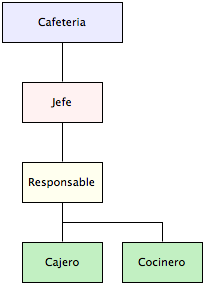
\includegraphics[width=0.3\textwidth]{img/organigrama}}
		\caption{Organigrama de una Cafetería}
		\label{fig:organigramaCafeteria}.
	\end{center}
\end{figure}

Así mismo se observa en la figura \ref{fig:actores} la presencia de un actor al que se le conoce como \getElementById[Stakeholder]{Agente} el cual hace referencia a un puesto de nuestra empresa \textbf{Loli Inc.} el cual pertenece al departamento de atención a usuarios, esto tomando como base el organigrama que se muestra en la figura \ref{fig:organigramaLoliInc}.

\begin{figure}[hbtp!]
	\begin{center}
		\fbox{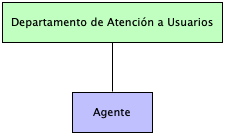
\includegraphics[width=0.3\textwidth]{img/organigramaLoliInc}}
		\caption{Organigrama de la empresa Loli Inc}
		\label{fig:organigramaLoliInc}
	\end{center}
\end{figure}


A continuación se realizan algunas observaciones correspondientes al diagrama en la figura \ref{fig:actores}:
	\begin{enumerate}
		\item El \getElementById[Stakeholder]{Persona} es un actor abstracto, que tiene como principal propósito abstraer las funcionalidades a las que todos las personas que utilicen el sistema tienen acceso sin depender directamente el rol que desempeñan. Por ejemplo, tanto el \getElementById{Cocinero} como el \getElementById{Cliente} tienen la misma posibilidad de Iniciar Sesión en el sistema o recuperar su cuenta de usuario asociada.
		\item El \getElementById[Stakeholder]{ResponsableDeLocal} es designado únicamente por el \getElementById{Jefe} y debe ser un empleado que puede o no tener el rol de \getElementById{Cocinero} o \getElementById{Cajero} en la misma cafetería.
	\end{enumerate}
	
	\begin{figure}[hbtp!]
	\begin{center}
		\fbox{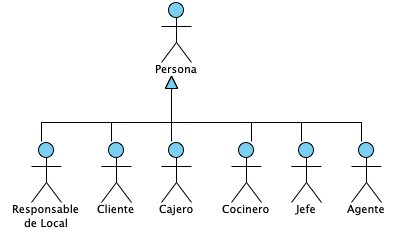
\includegraphics[width=0.5\textwidth]{img/actores}}
		\caption{Actores del Sistema}
		\label{fig:actores}
	\end{center}
\end{figure}


\begin{Actor}{Persona}{Persona}{Un usuario es toda persona que va a interactuar con el sistema mediante la aplicación móvil o la aplicación web.}
	\item[Responsabilidades:] No aplica.
	\item[Perfil]:\hspace{1pt}
		\begin{itemize}
			\item Alumno de nivel medio superior, superior o posgrado del I.P.N. o de U.N.A.M.
			\item Docente de nivel medio superior, superior o posgrado del I.P.N. o de U.N.A.M.
			\item Personal externo en una unidad académica del I.P.N. o escuela de la U.N.A.M.
			\item Personal de una cafetería.
		\end{itemize}
\end{Actor}


\begin{Actor}{Jefe}{Jefe}{También conocido como \textbf{Dueño} es la persona que legalmente tiene derecho a utilizar el nombre de una franquicia para abrir uno o más locales en determinados espacios, dentro o fuera de una unidad académica del I.P.N. así como una escuela de otra Institución Educativa.}
	\item[Responsabilidades:] \hspace{1pt}
		\begin{itemize}
			\item Agregar al sistema a los empleados.
			\item Designar un responsable del local.
			\item Tomar desiciones ejecutivas que respondan a las demandas de su establecimiento con base en 			gráficas o datos estadísticos.
			\item Definir las horas de operación de un local.
		\end{itemize}
	\item[Perfil]:\hspace{1pt}
		\begin{itemize}
			\item Licenciatura.
			\item Responsable.
			\item Líder.
		\end{itemize}
\end{Actor}

\begin{Actor}{ResponsableDeLocal}{Responsable de Local}{Es la persona designada por el \getElementById[Stakeholder]{Jefe} o Dueño para administrar o gestionar un local, recibir las entregas de productos de los proveedores con la facultad de delegar esta responsabilidad a otro empleado. }
	\item[Responsabilidades:] \hspace{1pt}
		\begin{itemize}
			\item Verificar que la integridad de los productos que llegan a la cafetería cumple con los acuerdos, reglamentos o estándares correspondientes.
			\item Definir las promociones que aplican a la cafetería de la que es responsable.
		\end{itemize}
	\item[Perfil]:\hspace{1pt}
		\begin{itemize}
			\item Licenciatura.
			\item Responsable.
			\item Confiable.
			\item Honesto.	
		\end{itemize}
\end{Actor}


\begin{Actor}{Cliente}{Cliente}{Es cualquier persona que va a una cafetería o local a consumir alimentos.}
	\item[Responsabilidades:]\hspace{1pt}
		\begin{itemize}
			\item Realizar el pago correspondiente a su pedido.
			\item Estar en el local al menos 5 minutos antes de que su pedido haya concluido su preparación.
			\item Revisar y responder a las notificaciones del sistema.
		\end{itemize}
	\item[Perfil:]\hspace{1pt}
		\begin{itemize}
		\item Alumno de nivel medio superior, superior o posgrado del I.P.N. o de U.N.A.M.
			\item Docente de nivel medio superior, superior o posgrado del I.P.N. o de U.N.A.M.
			\item Personal externo en una unidad académica del I.P.N. o escuela de la U.N.A.M.
		\end{itemize}
\end{Actor}


\begin{Actor}{Cocinero}{Cocinero}{Es una persona que pertenece a una cafetería y que tiene como principal responsabilidad atender pedidos y cocinarlos o delegarle esta responsabilidad a otro cocinero dentro de la misma cafetería.}
	\item[Responsabilidades:]\hspace{1pt}
		\begin{itemize}
			\item Monitoreo, control y conservación de los insumos de la cocina.
			
			\item Colaborar en la planificación de menús.
			
			\item Ayudar a administrar los costos e inventario.
			
			\item Dividir, conducir y organizar el trabajo con otros miembros del staff en la preparación de las ordenes.
			
			\item Iteractuar con el proveedor del servicio.
			
			\item Atender y preparar los pedidos solicitados por los clientes.
		\end{itemize}
	
	\item[Perfil:] \hspace{0.5cm}
		\begin{itemize}
			\item Excelentes habilidades de comunicación.
			
			\item Buenos estándares de higiene.
			
			\item Organizado y metódico.
			
			\item Experiencia en cáterin.
		\end{itemize}
\end{Actor}


\begin{Actor}{Cajero}{Cajero}{Es una persona que pertenece a una cafetería y que tiene como propósito cobrar los pedidos de los clientes.}
\item[Responsabilidades:] \hspace{0.5cm}
		\begin{itemize}
			\item Recibir dinero en efectivo, de requerirlo realiza arqueos de caja.
			
			\item Es el responsable directo de dinero en efectivo.
			
			\item Registrar operando una caja los movimientos de entrada y salida de dinero.
			
			\item Informar a su superior los movimientos diarios de la caja.
			
			\item Mantener en orden el equipo y sitio de trabajo, reportando cualquier anomalia.
			
			\item Manejar un grado de confidencialidad sobre las transacciones bajo.
		\end{itemize}
	
	\item[Perfil:] \hspace{0.5cm}
		\begin{itemize}
			\item Excelentes habilidades de comunicación , para atención al cliente.
			
			\item Habilidades numericas.
			
			\item Actitud de servicio.
			
			\item Proactivo.
			
			\item Responsable.
			
			\item Buena gestión de tiempo.
		\end{itemize}

\end{Actor}



\begin{Actor}{Administrador}{Administrador}{Es la persona que se encargará de desbloquear cuentas de usuario en el sistema así como de vigilar y mejorar las respuestas del sistema una vez sea puesto en producción.}
\item[Responsabilidades:]\hspace{1pt}
		\begin{itemize}
			\item Desbloquear cuentas de usuario.
		\end{itemize}
	\item[Perfil:]\hspace{1pt}
		\begin{itemize}
			\item Conocimiento en informática.
			\item Facilidad para comunicarse.
			\item Dominio y conocimiento básico de la funcionalidad del sistema.
		\end{itemize}

\end{Actor}



	
	\part{Modelo Estático}
	
	\chapter{Arquitectura Lógica}
	\label{ch:arq}
	%!TEX root = ../prueba.tex
En este capítulo se detallan los casos de uso correspondientes al módulo \varModulo y su interacción con los actores del sistema. El sistema está divido en dos subsistemas: una aplicación móvil y una aplicación web. Los casos de uso correspondientes a ambos módulos se pueden observar en la figura \ref{fig:arqLogica}
\begin{figure}[hbtp!]
	\begin{center}
		\fbox{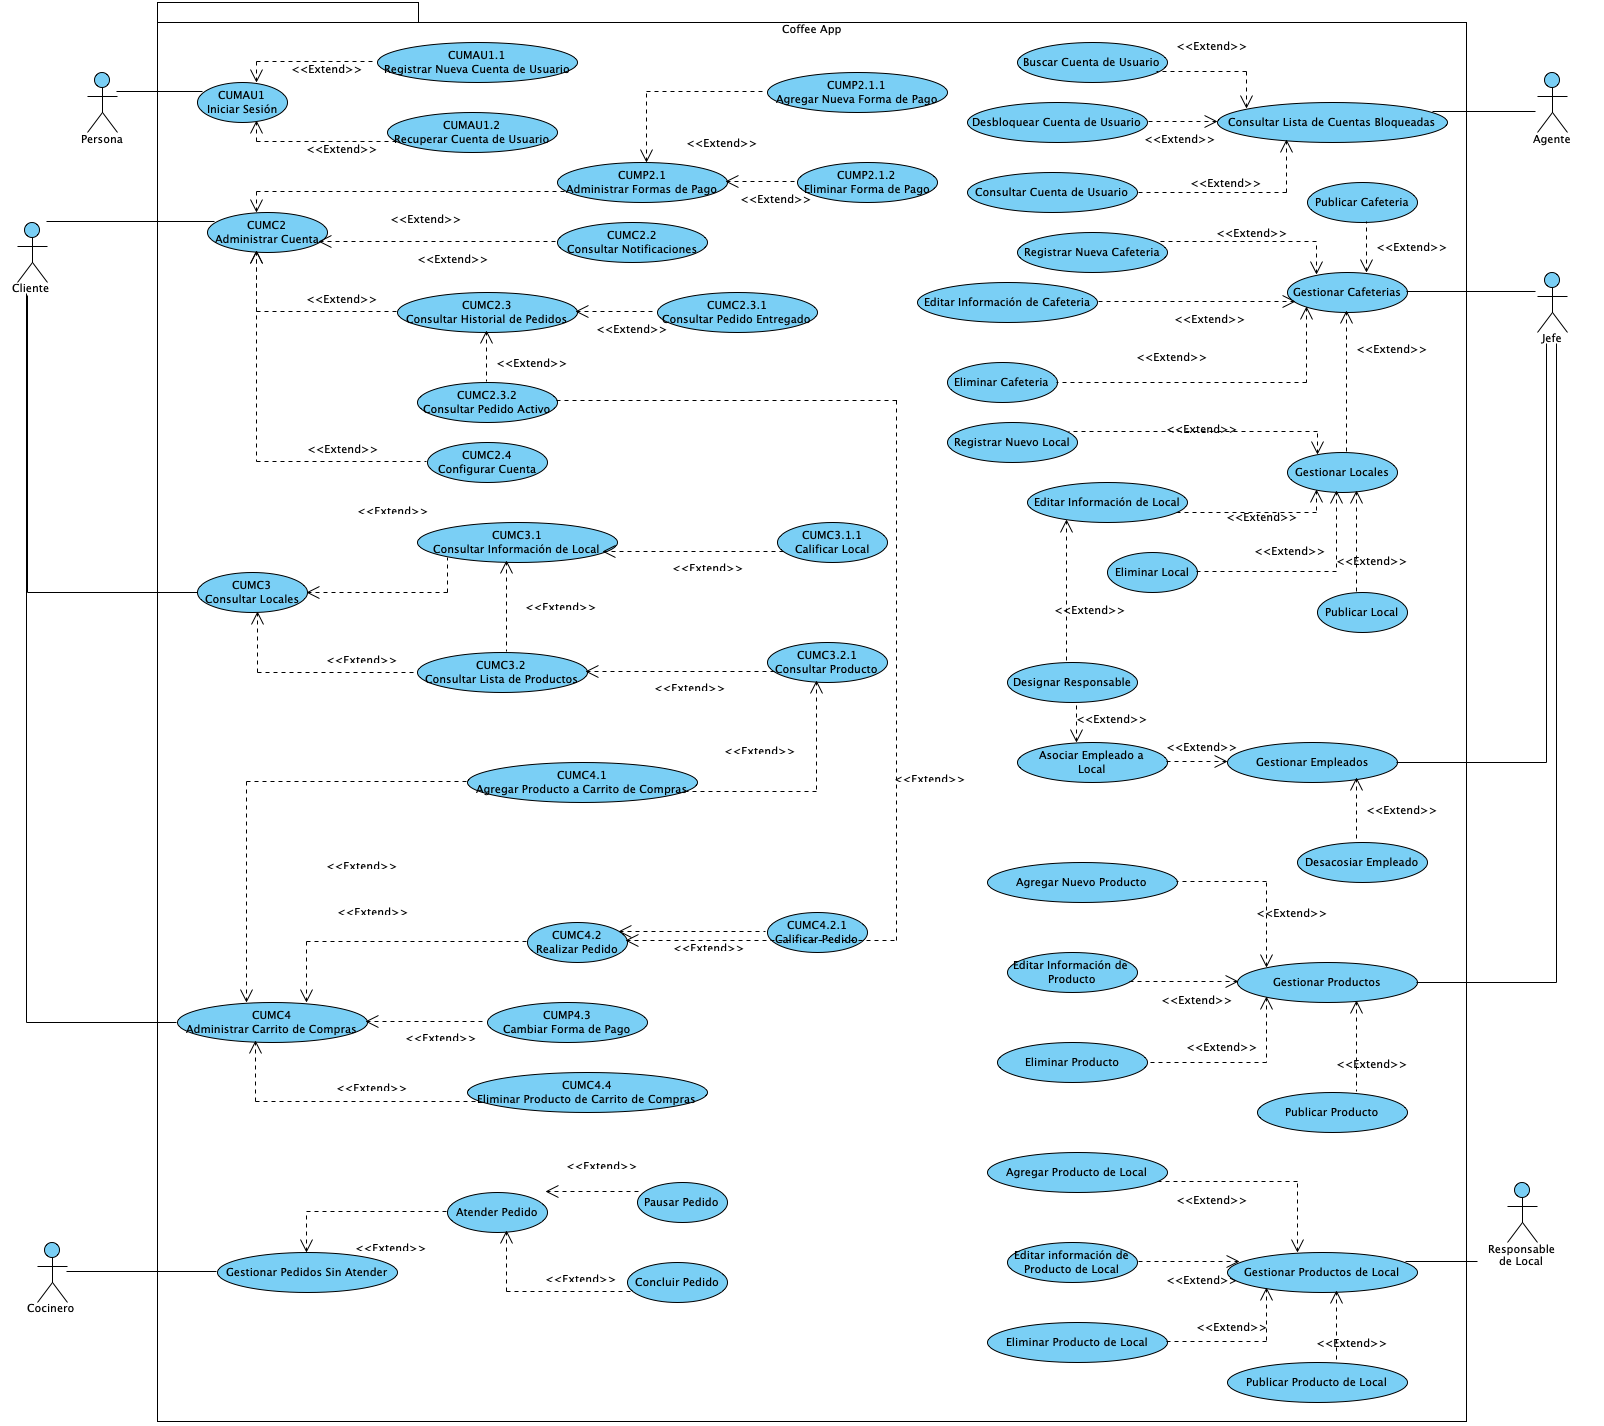
\includegraphics[width=0.7\textwidth]{img/arqLogica}}
		\caption{Arquitectura lógica del módulo \varModulo. Aplicación Móvil.}
		\label{fig:arqLogica}
	\end{center}
\end{figure}
	
	\chapter{Modelo de Información}
	\label{ch:modeloDeInformacion}
	En este capítulo se utiliza un diagrama de clases para mostrar la relación que existe en los tériminos y entidades de negocio descritas en el capítulo \ref{ch:glosario}. Estas relaciones están descritas con base en la especificación de \textit{UML} y en la base de datos del sistema.
	%!TEX root = ../prueba.tex

\begin{figure}[hbtp!]
	\begin{center}
		\fbox{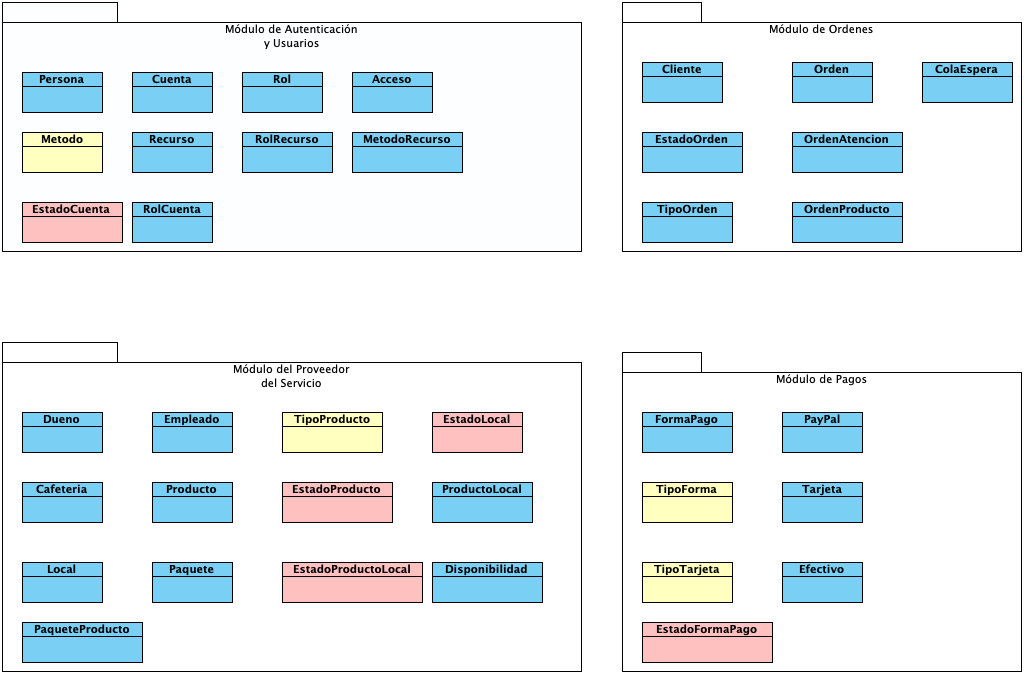
\includegraphics[width=0.5\textwidth]{img/MDI}}
		\caption{Modelo de Información del Sistema}
		\label{fig:mdi}
	\end{center}
\end{figure}
Como se puede observar en la figura \ref{fig:mdi}, el sistema está dividido por módulos, sus entidades serán descritas a continuación por medio de tablas además de que cada módulo se divide por secciones. Los atributos que no están presentes en la figura también son descritos a lo largo de este capítulo.

\section{Módulo de Autenticación y Usuarios}

En el módulo de autenticación y usuarios se encuentran aquellas entidades que permiten el acceso y registro al sistema.

\begin{figure}[hbtp!]
	\begin{center}
		\fbox{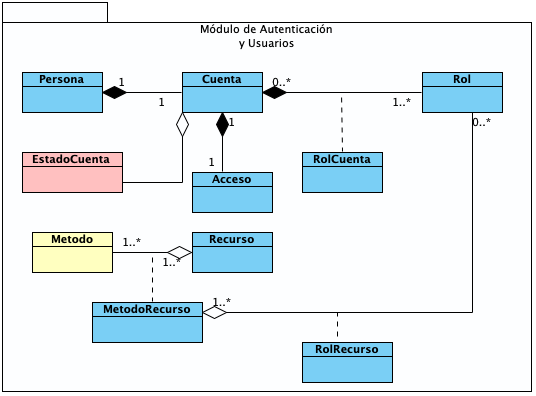
\includegraphics[width=0.7\textwidth]{img/MDI_MAU}}
		\caption{Modelo de Información del Módulo de Autenticación y Usuarios}
		\label{fig:mdimau}
	\end{center}
\end{figure}

\newpage
\begin{Entidad}{Persona}{Persona}
	\attr{nombre}{Nombre}{String}{ Nombre propio con el cual se identificara la persona.}{\datRequerido}
	\attr{primerApellido}{Primer Apellido}{String}{ Palabra que sigue despues del nombre de la persona. }{\datRequerido}
	\attr{segundoApellido}{Segundo Apellido}{String}{ Palabra que sigue despues del primer apellido de la persona. }{\datRequerido}
	\attr{foto}{Foto}{Byte[]}{ Foto del cliente.}{\datOpcional}
	\EntityRelSection
	\brRel{\brRelComposition}{Cuenta}{Una persona tiene una cuenta  con la que el cliente tendra acceso a la aplicación.}
	\brRel{\brRelComposition}{Persona}{Una persona tiene una cuenta para el ingreso al sistema.}
	\brRel{\brRelGeneralization}{Dueño}{El dueño es una persona}
	\brRel{\brRelGeneralization}{Empleado}{Un Empleado es una persona.}
\end{Entidad}
\newpage
\begin{Entidad}{Cuenta}{Cuenta}
	\attr{nombreDeUsuario}{Nombre de Usuario}{String}{ Palabra con la que se identificara el cliente. }{\datRequerido}
	\attr{correoElectronico}{Correo Electrónico}{String}{ Herramienta necesaria para mantener comunicación entre el usuario y la empresa, de modo que esta pueda brindar su mejor servicio. }{\datRequerido}
	\attr{contrasena}{Contraseña}{String}{ Cadena de caracteres elegidos por el usuario para el ingreso único a su cuenta. }{\datRequerido}
	\attr{fechaDeCreacion}{Fecha de Creación}{Timestamp}{Es la fecha en la cual se creo la cuenta de usuario del cliente. }{\datRequerido}
	\EntityRelSection
	\brRel{\brRelComposition}{Persona}{Una persona tiene una cuenta de usuario que le permite acceder a las funcionalidades del sistema con respecto a su rol.}
	\brRel{\brRelComposition}{Rol}{.}
	\brRel{\brRelComposition}{Acceso}{ El cliente accesa al sistema mediante su cuenta. }
	\brRel{\brRelAgregation}{Estado de Cuenta}{.}
\end{Entidad}

\begin{Entidad}{EstadoDeCuenta}{Estado de Cuenta}
	\attr{nombreDeEstado}{Nombre de Estado}{String}{ Estado en el que se encuentra la cuenta del cliente. }{\datRequerido}
	\EntityRelSection
	\brRel{\brRelComposition}{Cuenta}{ Una cuenta solo podra tener una forma de acceso en la aplicaccion.}

\end{Entidad}

\begin{Entidad}{Acceso}{Acceso}
	\attr{fechaDeUltimoAcceso}{fechaDeUltimoAcceso}{Timestamp}{ Fecha en la que se indicara cual fue la ultima vez que el cliente acceso a la aplicación. }{\datRequerido}
	\attr{numeroIntentos}{Número de Intentos}{Integer}{ Cantidad de veces que el usuario intentó ingresar a su cueta sin éxito alguno. }{\datRequerido}
	\EntityRelSection
	\brRel{\brRelComposition}{Cuenta}{El cliente accesa al sistema mediante su cuenta}
\end{Entidad}


%---------------------
\section{Módulo de Órdenes}
En el módulo de órdenes se le permite al \getElementById[Stakeholder]{Cliente} realizar pedidos a los locales que están registrados en el sistema.\\

\begin{figure}[hbtp!]
	\begin{center}
		\fbox{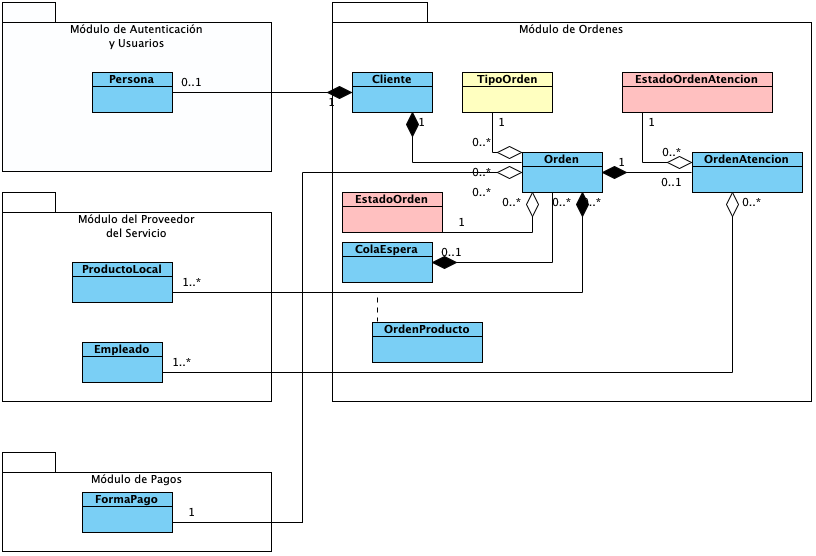
\includegraphics[width=0.5\textwidth]{img/MDI_ORD}}
		\caption{Modelo de Información del Módulo de Órdenes}
		\label{fig:mdiord}
	\end{center}
\end{figure}

\newpage
\begin{Entidad}{cliente}{Cliente}
	\EntityRelSection
	\brRel{\brRelAgregation}{Orden}{ El cliente puede realizar una o varias ordenes a un local.}
	\brRel{\brRelAgregation}{Persona}{Una persona tiene una cuenta para el ingreso al sistema.}
	\brRel{\brRelAgregation}{Forma de Pago}{El cliente podra elegir entre las distintas formas de pago con las que cuenta el sistema.}
\end{Entidad}

\begin{Entidad}{Orden}{Orden}
	\attr{fechaOrden}{Fecha de la Orden}{Date}{ Fecha en la que se realizó la orden. }{\datRequerido}
	\attr{fechaUltimaActualizacion}{Fecha Ultima Actualizacion}{Date}{ Fecha en la que se realizó la ultima modificacion a la Orden. }{\datRequerido}
	\attr{stConfirmacion}{Estado de Confirmación}{Boolean}{ Estado en donde se podra ver si la orden fue confirmada o rechazada. }{\datRequerido}
	\attr{stPrioridad}{Estado de Prioridad}{Integer}{ Estado en donde se vera la priodirad de la orden. }{\datRequerido}
	\EntityRelSection
	\brRel{\brRelComposition}{Cliente}{ El cliente puede realizar una o varias ordenes a un local.}
	\brRel{\brRelComposition}{Cola de Espera}{Una orden sera asignada a una cola de espera.}
	\brRel{\brRelComposition}{Estado de Orden}{ Una o muchas ordenes pueden tener el mismo estado.}
	\brRel{\brRelComposition}{Tipo de Orden}{ Una o muchas ordenes pueden pertenecer al mismo tipo de orden.}
	\brRel{\brRelComposition}{Orden en Atencion}{Una orden puede ser atendiada por un cocinero.}
	\brRel{\brRelComposition}{Producto en orden}{Producto que se encuentra dentro de una orden.}
	\brRel{\brRelComposition}{Produnto}{Un producto puede pertenecer a varias ordenes.}
	\brRel{\brRelAgregation}{Local}{Muchas ordenes pueden ser dirijidas a un local.}
\end{Entidad}

\begin{Entidad}{colaEspera}{Cola de Espera}
	\attr{fechaCola}{Fecha de Cola}{Date}{ Fecha en la que se inicio la cola de espera. }{\datRequerido}
	\attr{ultimaActualizacion}{Fecha Ultima Actualizacion}{Timestamp}{ Fecha de la actualizacion del estado de la cola de espera.}{\datRequerido}
	\EntityRelSection
	\brRel{\brRelComposition}{Orden}{Una orde sera asignada a una cola de espera.}
\end{Entidad}

\begin{Entidad}{estadoOrden}{Estado de Orden}
	\attr{nombreEstado}{Nombre del Estado}{String}{Estado en que se encuentra a Orden. }{\datRequerido}
	\EntityRelSection
	\brRel{\brRelAgregation}{Orden}{ Una o muchas ordenes pueden tener el mismo estado.}
\end{Entidad}

\begin{Entidad}{tipoOrden}{Tipo de Orden}
	\attr{nombreTipo}{Nombre del Tipo}{String}{ Tipo de Orden que se realizó. }{\datRequerido}
	\EntityRelSection
	\brRel{\brRelAgregation}{Orden}{Una o muchas ordenes pueden ppertenecer al mismo tipo de orden}
\end{Entidad}

\begin{Entidad}{ordenAtencion}{Orden en Atención}
	\EntityRelSection
	\brRel{\brRelComposition}{Orden}{Una orden debe ser atendida por un cocinero.}
	\brRel{\brRelAgregation}{Estado de Orden en Atención}{}
\end{Entidad}

\begin{Entidad}{estadoOrdenAtencion}{Estado de Orden en Atención}
	\attr{nombreEstado}{Nombre del Estado}{String}{ }{\datRequerido}
	\EntityRelSection
	\brRel{\brRelAgregation}{Orden en Atención}{}
\end{Entidad}

\begin{Entidad}{productoOrden}{Producto en Orden}
	\attr{comentario}{Comentario}{String}{ Comentario acerca del producto  }{\datRequerido}
	\attr{comentarioCalificacion}{Comentario de Calificación}{String}{ Calificacion con un intervalo de 0 a 5 acerca del producto  }{\datRequerido}
	\attr{nuRating}{Numero Rating}{Double}{ Numero en el que estara posicionado el producto, esto depende de la calificacion dada por los clientes. }{\datRequerido}
	\EntityRelSection
	\brRel{\brRelComposition}{Orden}{Producto que se encuentra dentro de una orden}
	\brRel{\brRelComposition}{Producto}{Producto al cual se le dara una calificación y un rating}
\end{Entidad}

%------------------------
\section{Modelo de Información del Módulo del Proveedor del Servicio}

En el módulo del proveedor del servicio se le permitee al \getElementById[Stakeholder]{Jefe} registrar en el sistema la información de cafeterías, de sus locales y de los productos que se ofertan en esos locales. Así mismo el \getElementById[Stakeholder]{ResponsableDeLocal} puede registrar la información de productos que se oferten únicamente en un local.

\begin{figure}[hbtp!]
	\begin{center}
		\fbox{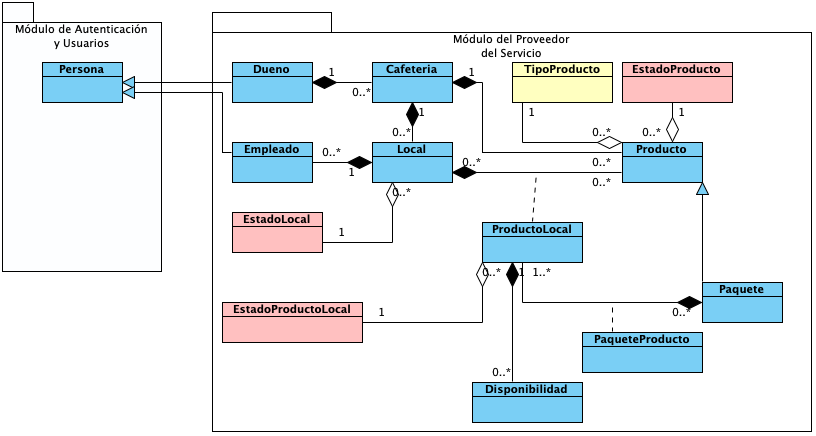
\includegraphics[width=0.5\textwidth]{img/MDI_MPS}}
		\caption{Modelo de Información del Módulo del Proveedor del Servicio}
		\label{fig:mdimps}
	\end{center}
\end{figure}

\newpage
\begin{Entidad}{dueño}{Dueño}
	\EntityRelSection
	\brRel{\brRelComposition}{Cafetería}{El dueño puede agregar una o muchas cafeterías al sistema}
	\brRel{\brRelGeneralization}{Persona}{El dueño es una persona}
\end{Entidad}

\begin{Entidad}{estadoProducto}{Estado de Producto}
	\attr{nombreEstado}{Nombre de Estado}{String}{ Estado en que se encuentra el producto. }{\datRequerido}
	\EntityRelSection
	\brRel{\brRelAgregation}{Producto}{Un estado de producto puede ser asignado a uno o muchos productos.}
\end{Entidad}
\newpage
\begin{Entidad}{cafeteria}{Cafetería}
	\attr{nombreCafeteria}{Nombre de Cafeteria}{String}{ Nombre con el cual se identificara la cafetería }{\datRequerido}
	\EntityRelSection
	\brRel{\brRelAgregation}{Producto}{ Una cafeteria puede tener uno o mas Productos a la venta para los clientes.}
	\brRel{\brRelComposition}{Dueño}{El dueño puede agregar una o muchas cafeterías al sistema}
	\brRel{\brRelComposition}{Local}{Una cafetería puede tener muchos locales.}
\end{Entidad}

\begin{Entidad}{tipoProducto}{Tipo Producto}
	\attr{tipo}{Tipo}{String}{ El el tipo al que pertenece el producto. }{\datRequerido}
	\EntityRelSection
	\brRel{\brRelAgregation}{Producto}{Muchos productos pueden pertenecer al mismo tipo.}
\end{Entidad}

\begin{Entidad}{producto}{Producto}
	\attr{nombreProducto}{Nombre del Producto}{String}{ Nombre con el cual se identificara el producto. }{\datRequerido}
	\attr{nuPrecioVenta}{Precio de Venta}{Double}{ Precio de venta que se le asignara al producto.}{\datRequerido}
	\attr{nuPrecioCompra}{Precio de Compra}{Double}{ Precio de compra que se le asignara al producto.}{\datRequerido}
	\EntityRelSection
	\brRel{\brRelComposition}{Cafetería}{ Un producto solo puede tener una cafetería.}
	\brRel{\brRelAgregation}{Estado de producto}{Un estado de produnto puede ser asignado a uno o muchos productos}
	\brRel{\brRelAgregation}{Tipo de Producto}{Muchos productos pueden pertenecer al mismo tipo.}
	\brRel{\brRelComposition}{Producto en Orden}{Producto al cual se le dara una calificacon y un rating.}
	\brRel{\brRelComposition}{Orden}{Un producto puede pertenecer a varias ordenes.}
	\brRel{\brRelGeneralization}{Producto de Local}{Un producto es aquel que se encuentra dentro de un local}
\end{Entidad}

\begin{Entidad}{estadoLocal}{Estado del Local}
	\attr{nombreEstado}{Nombre del Estado}{String}{ Estado en el que se encuetra el local. }{\datRequerido}
	\EntityRelSection
	\brRel{\brRelAgregation}{Local}{ Varios locales pueden pertenecer al mismo estado.}
\end{Entidad}

\begin{Entidad}{local}{Local}
	\attr{nombreLocal}{Nombre del Local}{String}{ Nombre con el que se identificara el Local }{\datRequerido}
	\attr{nuRating}{Rating}{Integer}{ Rating que tiene el local, esto depende de la calificacion que le den los clientes. }{\datRequerido}
	\attr{nuLongitud}{Longitud}{Double}{ Cordenadas geograficas del local. }{\datRequerido}
	\attr{nuLatitud}{Latitud}{Double}{ Cordenadas geograficas del local. }{\datRequerido}
	\attr{foto}{Foto}{Byte[]}{ Foto del Local para que el cliente pueda identificarlo.}{\datRequerido}
	\attr{horaInicio}{Hora de Inicio}{Time}{ Hora en la que el Local comienza a dar servicio.}{\datRequerido}
	\attr{horaFin}{Hora de Fin}{Time}{ Hora en la que el Local termina de dar servicio.}{\datRequerido}
	\EntityRelSection
	\brRel{\brRelComposition}{Cafetería}{Una cafetería puede tener muchos locales.}
	\brRel{\brRelAgregation}{Producto de Local}{Un local puede contar con ningun o productos.}
	\brRel{\brRelAgregation}{Orden}{Muchas ordenes pueden ser dirijidas a un local.}
	\brRel{\brRelComposition}{Responsable}{Solo habra un responsable en el local.}
	\brRel{\brRelComposition}{Empleado}{Varios empreados pueden estar asignados a un local.}
\end{Entidad}

\begin{Entidad}{productoLocal}{Producto del Local}
	\EntityRelSection
	\brRel{\brRelComposition}{Paquete}{Un paquete puede estar compuesto por varios productos.}
	\brRel{\brRelComposition}{Producto en paquete}{Producto que esta dentro de un paquete.}
	\brRel{\brRelGeneralization}{Producto}{Un producto es aquel que se encuentra dentro de un local.}
	\brRel{\brRelGeneralization}{Paquete}{Un paquete es un producto que esta dentro de un local.}
	\brRel{\brRelAgregation}{Estado Producto de Local}{Muchos productos del local pueden ser aasignados al mismo estado}
	
\end{Entidad}

\begin{Entidad}{empleado}{Empleado}
	\EntityRelSection
	\brRel{\brRelComposition}{Local}{Varios empleados pueden estar asignados a un local.}
	\brRel{\brRelGeneralization}{Persona}{Un espleado es una persona.}
	\brRel{\brRelGeneralization}{Orden de Atención}{Un empleado puede atender una orden.}
\end{Entidad}

\begin{Entidad}{responsable}{Responsable}
	\EntityRelSection
	\brRel{\brRelComposition}{Local}{Solo habra un responsable en el local.}
	\brRel{\brRelGeneralization}{Empleado}{El responsable es un empleado}
\end{Entidad}

\begin{Entidad}{estadoProductoLocal}{Estado Producto de Local}
	\attr{nombreEstado}{Nombre del Estado}{String}{ Estado en que se encuentra el producto. }{\datRequerido}
	\EntityRelSection
	\brRel{\brRelAgregation}{Producto de Local}{Muchos productos del local pueden ser aasignados al mismo estado}
\end{Entidad}

\begin{Entidad}{productoPaquete}{Producto en Paquete}
	\EntityRelSection
	\brRel{\brRelComposition}{Paquete}{Producto que esta dentro de un paquete}
	\brRel{\brRelComposition}{Producto de Local}{}
\end{Entidad}

\begin{Entidad}{paquete}{Paquete}
	\EntityRelSection
	\brRel{\brRelComposition}{Producto local}{Un paquete puede estar compuesto por varios productos}
	\brRel{\brRelGeneralization}{Producto de Local}{El paquete es un producto que esta en el local.}
\end{Entidad}

%--------------
\section{Modelo de Información del Módulo de Pagos}

En el módulo de pagos se le permite al \getElementById[Sstakeholder]{Cliente} agregar, editar o eliminar los métodos con los que puede realizar el pago de sus ordenes.

\begin{figure}[hbtp!]
	\begin{center}
		\fbox{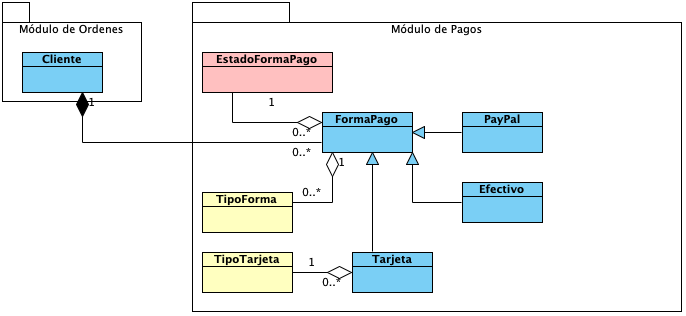
\includegraphics[width=0.5\textwidth]{img/MDI_PGS}}
		\caption{Modelo de Información del Módulo de Pagos}
		\label{fig:mdimpg}
	\end{center}
\end{figure}

\newpage
\begin{Entidad}{tipoForma}{Tipo de Forma de Pago}
	\attr{nombreTipo}{Nombre del Tipo}{String}{ Nombre con el que se identificara el tipo de pago. }{\datRequerido}
	\EntityRelSection
	\brRel{\brRelAgregation}{Forma de Pago}{Varias formas de pago pueden ser del mismo tipo.}
\end{Entidad}

\begin{Entidad}{paypal}{Paypal}
	\attr{correoElectronico}{Correo Electronico}{String}{ Correo electronico con el cual se registro en el sistema.}{\datRequerido}
	\attr{contraseña}{Contraseña}{String}{ Contraseña del usuario que utilza para acceder al sistema.}{\datRequerido}
	\EntityRelSection
	\brRel{\brRelGeneralization}{Forma de Pago}{Paypal es una forma de pago con la que se puedo realizar la compra de un producto.}
\end{Entidad}

\begin{Entidad}{formaPago}{Forma de Pago}

	\EntityRelSection
	\brRel{\brRelComposition}{Cliente}{Un cliente tiene una o varias formas de pago.}
	\brRel{\brRelAgregation}{Orden}{Una orden puede se puede pagar por varias formas de pago.}
	\brRel{\brRelAgregation}{Tipo de Forma de Pago}{Varias formas de pago pueden ser del mismo tipo.}
	\brRel{\brRelGeneralization}{Efectivo}{El efectivo es una forma de pago con la que se puede realizar la compra de un producto}
	\brRel{\brRelGeneralization}{Paypal}{Payoal es una forma de pago con la que se puede realizar la compra de un producto}
	\brRel{\brRelGeneralization}{Tarjeta}{El uso de la tarjeta de credito es una forma de pago con la que se puede realizar la compra de un producto}
\end{Entidad}

\begin{Entidad}{efectivo}{Efectivo}
	\EntityRelSection
	\brRel{\brRelGeneralization}{Forma de Pago}{El efectivo es una forma de pago con la que se puede realizar la compra de un producto}
\end{Entidad}

\begin{Entidad}{tarjeta}{Tarjeta}
	\attr{numeroTarjeta}{Numero de Tarjeta}{String}{ 16 digitos para la identificacion de la tarjeta. }{\datRequerido}
	\attr{fechaVencimiento}{Fecha de Vencimiento}{Date}{ Fecha en la que la tarjeta expira}{\datRequerido}
	\attr{claveSeguridad}{Clave de Seguridad}{String}{ Calve unica para la verificacion de los datos de la tarjeta.}{\datRequerido}
	\EntityRelSection
	\brRel{\brRelGeneralization}{Forma de pago}{El uso de la tarjeta de credito es una forma de pago con la que se puedo realizar la compra de un producto.}
	\brRel{\brRelAgregation}{Tarjeta}{Una Tarjeta tiene solo un tipo de tajeta.}
\end{Entidad}

\begin{Entidad}{tipoTarjeta}{Tipo de Tarjeta}
	\attr{nombreTipo}{Nombre del Tipo}{String}{ Nombre del tipo de tarjeta que se esta utilizando }{\datRequerido}
	\EntityRelSection
	\brRel{\brRelAgregation}{Tarjeta}{Una Tarjeta tiene solo un tipo de tajeta.}
\end{Entidad}



	
	\chapter{Reglas de Negocio}
	\label{ch:reglas}
	%!TEX root = ../prueba.tex

\section{Reglas de negocio}

\subsection{Reglas dde Negocio Generales}

En este capítulo se detallan las reglas de negocio que rigen al módulo de \varModulo y que el sistema deberá utilizar para controlar el acceso de los usuarios a las diferentes funcionalidades del sistema.

%**************************BR001********************************
\begin{BusinessRule}{BR001}{Campos obligatorios}{}{}{}
	\BRItem[Versión] 1.0
	\BRItem[Estado] Propuesta.
	\BRItem[Propuesta por] Diana Laura Mejía Mendoza.
	\BRItem[Revisada por] Pendiente.
	\BRItem[Aprobada por] Pendiente.
	\BRItem[Descripción] Los datos proporcionados en el sistema marcados como requeridos, no se deben omitir.
	\BRItem[Sentencia] Sea un $Campo$ marcado como $Obligatorio$, $ |  campo.obligatorio = true$ 
	$ \therefore \forall campo \Rightarrow campo.valor \neq \emptyset $

	\BRItem[Ejemplo] Para iniciar sesión en el sistema \textbf{Coffee App}, el actor introducé todos los datos en los campos \textbf{Usuario} y \textbf{Contraseña} marcados como obligarios. 

\end{BusinessRule}

%**************************BR002********************************

\begin{BusinessRule}{BR002}{Información correcta}{}{}{}
	\BRItem[Versión] 1.0.
	\BRItem[Estado] Propuesta.
	\BRItem[Propuesta por] Diana Laura Mejía Mendoza.
	\BRItem[Revisada por] Pendiente.
	\BRItem[Aprobada por] Pendiente.
	\BRItem[Descripción] Todos los datos proporcionados al sistema deben pertenecer al tipo de dato establecido en el modelo de información.
	\BRItem[Sentencia] Sea $F:$ Una expresión regular que determina el formato que un campo debe cumplir con base en el modelo de información. \\ $Dato$ Los datos ingresados por el actor, en un campo del sistema.\\
	
	Si $ Dato \in F \Longrightarrow InformacionCorrecta $
	\BRItem[Ejemplos]
		\begin{itemize}
			\item El actor introduce su Nombre que contiene solo carácteres alfabéticos.
			\item El actor introduce un número de celular, el cuál solamente contiene caractéres númericos.
			\item El actor introduce un correo electrónico que contiene un símbolo '@' y cuya terminación es un dominio de correo electrónico.
		\end{itemize}

\end{BusinessRule}

%**************************BR003********************************

\begin{BusinessRule}{BR003}{Eliminación lógica de elementos}{}{}{}
	\BRItem[Versión] 1.0.
	\BRItem[Estado] Propuesta.
	\BRItem[Propuesta por] Diana Laura Mejía Mendoza.
	\BRItem[Revisada por] Pendiente.
	\BRItem[Aprobada por] Pendiente.
	\BRItem[Descripción] Un elemento sólo se puede eliminar si no tiene asociaciones con otros elementos. 

	\BRItem[Sentencia]  Si $E_x \in E_y \Longrightarrow NoSePuedeEliminarElemento$ \\
	
	Donde: $E_x  \wedge E_y$: Elementos registrados en el sistema.

	\BRItem[Ejemplos]
	\begin{itemize}
		\item Una cafetería que tiene registrados productos no se puede eliminar.
		\item Se puede eliminar la cafetería si y solo si no tiene ningún producto registrado.
	\end{itemize}

\end{BusinessRule}

%**************************BR004********************************

\begin{BusinessRule}{BR004}{Unicidad de elementos}{}{}{}
	\BRItem[Versión] 1.0.
	\BRItem[Estado] Propuesta.
	\BRItem[Propuesta por] Diana Laura Mejía Mendoza.
	\BRItem[Revisada por] Pendiente.
	\BRItem[Aprobada por] Pendiente.
	\BRItem[Descripción] Un elemento no se puede duplicar en el ámbito donde es utilizado ni registrarse más de una vez. Dada la sentencia se consideran dentro de la regla las siguientes entidades y atributos:

	\begin{itemize}
		\item Cafetería, \{nombre\}
		\item Producto, \{nombre\}
	\end{itemize}
	\BRItem[Sentencia] Sea $ E_1, E_2$: Entidades utilizadas en un mismo ámbito. \\
	$A$: Atributo de una entidad. \\
	 $ | \forall  (A \in E_1) \neq (A \in E_2)$.

	\BRItem[Ejemplo]
		\begin{itemize}
			\item Dos cafeterías con diferentes nombres.
			\item Cafetería El Kiosquito.
			\item Cafetería Zen Garden
		\end{itemize}

\end{BusinessRule}

%Negocio


%**********************************************************
\subsection{Reglas de Negocio}
%**********************************************************


%**************************BR-MAU001********************************

\begin{BusinessRule}{BR-MAU001}{Número máximo de intentos}{}{}{}
	\BRItem[Versión] 1.0.
	\BRItem[Estado] Propuesta.
	\BRItem[Propuesta por] Diana Laura Mejía Mendoza.
	\BRItem[Revisada por] Pendiente.
	\BRItem[Aprobada por] Pendiente.
	\BRItem[Descripción]El número máximo de intentos fallidos para ingresar al sistema será de 3, de lo contrario la cuenta se bloqueará hasta que el administrador cambie el estado de la cuenta.
	
	\BRItem[Sentencia] Sea $Num_I$: Número de intentos que el usuario realiza para ingresar al sistema. \\

	Si $Num_I = 3 \Longrightarrow CuentaBloqueada$.


\end{BusinessRule}

%**************************BR-MAU002********************************

\begin{BusinessRule}{BR-MAU002}{Sesión activa}{}{}{}


\end{BusinessRule}

%**************************BR-MAU003********************************

\begin{BusinessRule}{BR-MAU003}{Contraseña válida}{}{}{}
	\BRItem[Versión] 1.0.
	\BRItem[Estado] Propuesta.
	\BRItem[Propuesta por] Eric Alejandro López Ayala.
	\BRItem[Revisada por] Pendiente.
	\BRItem[Aprobada por] Pendiente.
	\BRItem[Descripción] Una constraseña únicamente sera válida si tiene una longitud mínima de 8 carácteres, contiene al menos un carácter mayúscula, un carácter minúscula, un dígito y alguno de los siguientes carácteres especiales: '.' ',' '-' '\_'
	\BRItem[Sentencia] Sea $F:$ Una expresión regular que determina el formato que un campo debe cumplir con base en el modelo de información. \\ $Dato$ Los datos ingresados por el actor, en un campo del sistema.\\
	
	Si $ Dato \in F \Longrightarrow ContrasenaValida $
	\BRItem[Ejemplos]
	\begin{itemize}
		\item El actor introduce una contraseña de al menos 8 caráteres de longitud e incluye al menos un carácter minúscula, un carácter mayúscula, un dígito y alguno de los siguientes carácteres especiales: '.' ',' '-' '\_'
	\end{itemize}
	
\end{BusinessRule}

%**************************BR-MC005********************************

\begin{BusinessRule}{BR-MC005}{Calificación de un producto}{}{}{}
	\BRItem[Versión] 1.0.
	\BRItem[Estado] Propuesta.
	\BRItem[Propuesta por] Diana Laura Mejía Mendoza.
	\BRItem[Revisada por] Pendiente.
	\BRItem[Aprobada por] Pendiente.
	\BRItem[Descripción] Cada producto ofertado en un local tendrá una calificación, sólo un \textbf{Cliente} o una \textbf{Persona} que realizó la compra y se le entrego el producto podrá calificarlo. Así mismo, se pueden realizar $n$ calificaciones por persona del mismo producto, esto será con base en las veces que compró y se le entregó el producto.
	\BRItem[Sentencia] 
	
\end{BusinessRule}

%**************************BR-MC007********************************

\begin{BusinessRule}{BR-MC007}{Notificaciones}{}{}{}
	\BRItem[Versión] 1.0.
	\BRItem[Estado] Propuesta.
	\BRItem[Propuesta por] Diana Laura Mejía Mendoza.
	\BRItem[Revisada por] Pendiente.
	\BRItem[Aprobada por] Pendiente.
	\BRItem[Descripción] Cada producto ofertado en un local tendrá una calificación, sólo un \textbf{Cliente} o una \textbf{Persona} que realizó la compra y se le entrego el producto podrá calificarlo. Así mismo, se pueden realizar $n$ calificaciones por persona del mismo producto, esto será con base en las veces que compró y se le entregó el producto.
	\BRItem[Sentencia] 
	
\end{BusinessRule}

%**************************BR-MC008********************************

\begin{BusinessRule}{BR-MC008}{Clasificación de notificaciones}{}{}{}
	\BRItem[Versión] 1.0.
	\BRItem[Estado] Propuesta.
	\BRItem[Propuesta por] Diana Laura Mejía Mendoza.
	\BRItem[Revisada por] Pendiente.
	\BRItem[Aprobada por] Pendiente.
	\BRItem[Descripción] Cada producto ofertado en un local tendrá una calificación, sólo un \textbf{Cliente} o una \textbf{Persona} que realizó la compra y se le entrego el producto podrá calificarlo. Así mismo, se pueden realizar $n$ calificaciones por persona del mismo producto, esto será con base en las veces que compró y se le entregó el producto.
	\BRItem[Sentencia] 
	
\end{BusinessRule}
	
	\part{Modelo Dinámico}
	
	\chapter{Máquinas de Estado}
	\label{ch:maquinas}
	%!TEX root = ../prueba.tex
En el presente capítulo se realiza la especificación de las máquinas o autómatas finitos que describen:
	\begin{Citemize}
		\item Comportamiento de operaciones sobre actores, términos o entidades de negocio.
		\item Ciclo de Vida de objetos o entidades de negocio.
	\end{Citemize}

Cada máquina de estado tiene una descripción así como los casos de uso asociados a la máquina, también se utiliza un diagrama donde se utiliza la notación U.M.L. para las máquinas de estado.

\begin{Maquina}{MAQMAU01}{Máquina de Estado de la Cuenta de Usuario de una Persona}

\subsection{Resumen}

En cualquier momento dado, la cuenta de un usuario tiene un ’estado’ el  sistema. Las acciones que los actores pueden realizar dependen de dicho estado y pueden tener como consecuencia la transición a otro estado. Los estados y transiciones posibles se muestran en la 	\ref{fig:maqmau01} y se describen a continuación.
	\subsection{Descripción}
	El ciclo de vida de la cuenta de usuario de una  \getElementById[Stakeholder]{Persona} se describe a continuación:
		\begin{description}
			\item[Activo] Este es el estado inicial donde  una persona se registra en el sistema por medio de la aplicación web o la aplicación móvil\footnote{Ver \getElementById[CU]{CUMAU1}} y se le asocia una cuenta de usuario con este estado, el cual permite que la persona acceda a todas las funcionalidades del sistema desde cualquier punto de entrada. Estar en este estado implica:
			
			\begin{Titemize}
			\Titem \getElementById[Stakeholder]{Persona}: 	Este usuario puede: Iniciar sesión en el sistema "Coffee App" por medio de la aplicación web o móvil.
			\end{Titemize}
			
			\item[Bloqueado] Cuando un Usuario con estado \textbf{Activo} ha intentado ingresar al sistema por el control de acceso y se ha equivocado tres veces al ingresar su usuario y/o contraseña, el estado de la cuenta de usuario cambiará a \textbf{Bloqueado}. Estar en este estado implica:
			
			\begin{Titemize}
			\Titem \getElementById[Stakeholder]{Administrador}: 	Este usuario puede: Con base en su criterio, cambiar el estado de la cuenta de usuario a \textbf{Activo}
			\end{Titemize}
			
		\end{description}
	El diagrama correspondiente a la descripción previa se puede observar en la figura \ref{fig:maqmau01}.
	\begin{figure}[hbtp!]
	\begin{center}
		\fbox{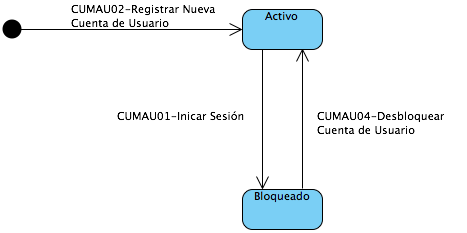
\includegraphics[width=0.7\textwidth]{maquinas/maq-mau01}}
		\caption{Ciclo de Vida de la Cuenta de Usuario de una Persona}
		\label{fig:maqmau01}
		\end{center}
	\end{figure}

\end{Maquina}

\begin{Maquina}{MAQORDEN}{Máquina de Estado de una Orden}
	\subsection{Descripción}
	En cualquier momento dado, una orden tiene un 'estado' en el sistema. Las acciones que los actores pueden realizar sobre una orden dependen de dicho estado y pueden tener como consecuencia la transición a otro estado. Los estados y transiciones posibles se muestran en la figura 	\ref{fig:maqorden} y se describen a continuación.
		\begin{description}
			\item[Confirmado] Es el estado inicial en el que una orden ya ha sido confirmada por un \getElementById[Stakeholder]{Cliente} o una \getElementById[Stakeholder]{Persona} y pasa a la gestión de pedidos de los cocineros para que algún \getElementById[Stakeholder]{Cocinero} pueda comenzar a preparar el pedido, estar en este estado implica que:

		\item \getElementById[Stakeholder]{Cocinero}: Este usuario puede:
		\begin{itemize}
			\item Visualizar la orden y por lo tanto los productos solicitados por un cliente o una persona. 
			\item Comenzar la preparación de la orden. 
		\end{itemize}
		
			\item[Cancelado] Cuando una orden por 
		\end{description}
	\begin{figure}[hbtp!]
	\begin{center}
		\fbox{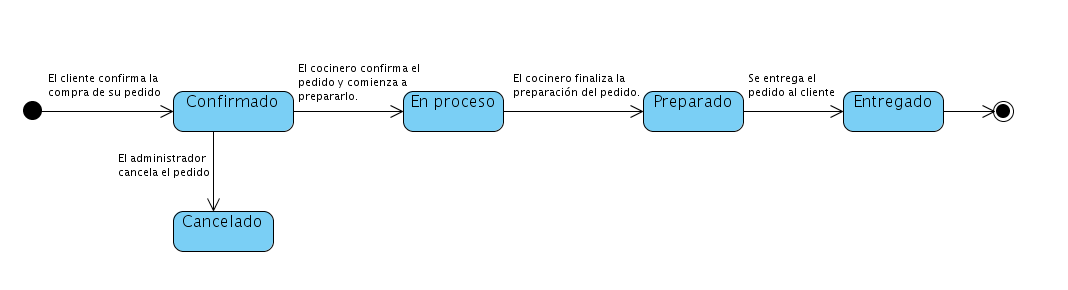
\includegraphics[width=0.7\textwidth]{maquinas/maq-orden}}
		\caption{Ciclo de Vida de una Orden}
		\label{fig:maqorden}
		\end{center}
	\end{figure}

\end{Maquina}


\begin{Maquina}{MAQLOCAL}{Máquina de Estado de un Local}
	\subsection{Descripción}
	En cualquier momento dado, un local tiene un 'estado' en el sistema. Las acciones que se pueden realizar sobre un local dependen de dicho estado y pueden tener como consecuencia la transición a otro estado. Los estados y transiciones posibles se muestran en la figura 	\ref{fig:maqlocal} y se describen a continuación.
			\begin{description}

			\item[Confirmado] Es el estado inicial en el que una orden ya ha sido confirmada por un \getElementById[Stakeholder]{Cliente} o una \getElementById[Stakeholder]{Persona} y pasa a la gestión de pedidos de los cocineros para que algún \getElementById[Stakeholder]{Cocinero} pueda comenzar a preparar el pedido, estar en este estado implica que:
		\item \getElementById[Stakeholder]{Cocinero}: Este usuario puede:
		\begin{itemize}
			\item Visualizar la orden y por lo tanto los productos solicitados por un cliente o una persona. 
			\item Comenzar la preparación de la orden. 
		\end{itemize}
		
			\item[Cancelado] Cuando una orden por 
		\end{description}
	\begin{figure}[hbtp!]
	\begin{center}
		\fbox{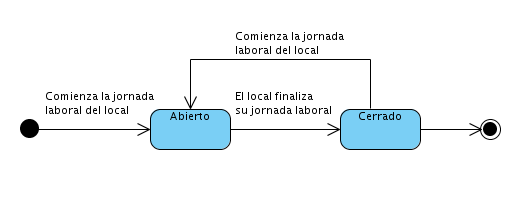
\includegraphics[width=0.7\textwidth]{maquinas/maq-local}}
		\caption{Ciclo de Vida de un Local}
		\label{fig:maqlocal}
		\end{center}
	\end{figure}

\end{Maquina}



\begin{Maquina}{MAQPRODUCTO}{Máquina de Estado de un Producto}
	\subsection{Descripción}
	En cualquier momento dado, un producto tiene un 'estado' en el sistema. Las acciones que se pueden realizar sobre un producto dependen de dicho estado y pueden tener como consecuencia la transición a otro estado. Los estados y transiciones posibles se muestran en la figura 	\ref{fig:maqproducto} y se describen a continuación.
				\begin{description}

			\item[Disponible] Es el estado inicial en el que un producto se encuentra en existencia en un determinado local, estar en este estado implica que:
		\item \getElementById[Stakeholder]{Cliente} o \getElementById[Stakeholder]{Persona}: Los  usuarios pueden:
		\begin{itemize}
			\item Visualizar los productos que esten disponibles.
			\item Agregar al carrito de compras los productos que esten disponibles y que sean de su interes.
						
		\end{itemize}
		
		\item \getElementById[Stakeholder]{Administrador} : El usuario puede:
		\begin{itemize}
			\item Cambiar el estado del producto a \textbf{Agotado}.
						
		\end{itemize}
		
			\item[Agotado] Cuando una orden por 
		\end{description}
	\begin{figure}[hbtp!]
	\begin{center}
		\fbox{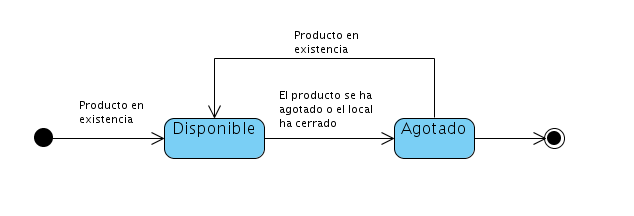
\includegraphics[width=0.7\textwidth]{maquinas/maq-producto}}
		\caption{Ciclo de Vida de un Producto}
		\label{fig:maqproducto}
		\end{center}
	\end{figure}

\end{Maquina}
	
	\chapter{Casos de Uso}
	En este capítulo se encuentra la descripción de los casos de uso que se encuentran del lado izquierdo de la figura \ref{fig:arqLogica}, es decir, a los que hacen referencia únicamente a la aplicación móvil. La descripción de los casos de uso se hace con base en el documento \textit{E1-Especificación del Proyecto} en donde se pueden encontrar los requerimientos funcionales del sistema. Es importante mencionar que los casos de uso fueron escritos utilizando un enfoque \textit{Black Box}.
	\label{ch:casosDeUso}
	%!TEX root = ../prueba.tex
En este capítulo están contenidos los casos de uso.
%
%!TEX root = ../../prueba.tex

\begin{UseCase}{CUMC07}{Consultar producto}{
Permite visualizar la información general de un producto para que una \getElementById[Stakeholder]{Persona} o un \getElementById[Stakeholder]{Cliente} se percate si el producto de interes, es el que el requiere. \\  
Es importante saber si el producto está diponible o se ha agotado ya que solo podrá visualizar la descripción general del producto si se encuentra disponible. \\ Un producto pasa al estado \textbf{Agotado}, debido a que en el local se terminó la existencia de dicho producto, o el local donde ofertan el producto ha finalizado su jornada laboral. \\
Por otra parte al consultar la información del producto se podrá visualizar el promedio de la calificación que le han otorgado, es importante ya que ayuda a incrementar la referencia que tiene este producto y así con base en la calificación y el criterio del cliente realice su compra.\\
Una gran 
}
	\UCitem{Versión}{0.1}
	\UCitem{Elaboró}{Diana Laura Mejía Mendoza}
	\UCitem{Supervisó}{Francisco Isidoro Mera Torres}
	\UCitem{Prioridad}{Alta}
	\UCitem{Complejidad}{Media}
	\UCitem{Volatilidad}{Baja}
	\UCitem{Madurez}{Media}
	\UCsection{Atributos}
	\UCitem{Actor}{\begin{Titemize}
	\Titem \getElementById[Stakeholder]{Persona}
	\Titem \getElementById[Stakeholder]{Cliente}
	\end{Titemize}}
	\UCitem{Propósito}{Proporcionar un mecanismo .}
	\UCitem{Entradas}{\begin{Titemize}
		\Titem \getElementById[Entidad]{Cuenta.nombreDeUsuario}.
		\Titem \getElementById[Entidad]{Cuenta.contrasena}.
		\Titem \getElementById[Entidad]{Acceso.numeroIntentos}.
	\end{Titemize}}
	\UCitem{Salidas}{\begin{Titemize}
		\Titem \getElementById[MSG]{MSG03}
	\end{Titemize}}
	\UCitem{Precondiciones}{\begin{Titemize}
		\Titem La persona que va a ingresar al sistema debe estar registrada en el sistema.
		\Titem No debe existir una sesión activa.
	\end{Titemize}}	
	\UCitem{Postcondiciones}{\begin{Titemize}
		\Titem La persona tiene acceso a la página de bienvenida que le corresponde a su 
		\Titem La persona tiene
	\end{Titemize}}
	\UCitem{Reglas de Negocio}{
		\begin{Titemize}
			\Titem \getElementById[BR]{BR-MAU01}
		\end{Titemize}
	}
	\UCitem{Errores}{
		\begin{Titemize}
			\Titem \UCerr{Uno}{Los campos marcados en el formulario como obligatorios están vacíos}{se muestra el mensaje \getElementById[MSG]{MSG02}}
		\end{Titemize}
	}
	\UCitem{Viene de}{No aplica.}
	\end{UseCase}
	
	
	\begin{UCtrayectoria}
		\UCpaso[\UCactor] Solicita consultar la información de un producto dando clic en el producto deseado de la pantalla \getElementById[UIMC07]{Carrito de compras}.
		\UCpaso Verifica que el estado del producto sea \textbf{Disponible} con base en el \textbf{Modelo de ciclo de vida de un producto}.\refErr{Uno}
		\UCpaso Obtiene la foto, el nombre, la descripción y precio del producto seleccionado.
		\UCpaso Obtiene el promedio de la calificación que los clientes han asignado al producto con base en la regla de negocio \textbf{REGLA DE NEGOCIO}.
		\UCpaso Habilita el campo \textbf{Ingresar nota}.
		\UCpaso Muestra la pantalla \getElementById[UIMC07]{Consultar producto} con la información obtenida.
		\UCpaso [\UCactor] Ingresa la información solicitada.
		\UCpaso [\UCactor] \label{ConsultarProducto-Productos} Selecciona el número de productos que requiere comprar.
		\UCpaso Calcula el total de dinero con base en los productos solicitados en el paso \ref{ConsultarProducto-Productos}
		\UCpaso [\UCactor] Solicita agregar el producto a su carrito de compras presionando el botón \IUbutton{Agregar al carrito}.\refTray{B}
		\UCpaso Verifica que exista la cantidad de productos solicitados con base en la regla de negocio \textbf{REGLA DE NEGOCIO}.\refTray{C}
		\UCpaso Muestra la pantalla \getElementById[UIMC07]{Carrito de compras}.
	\end{UCtrayectoria}
	

	\begin{UCtrayectoriaA}{A}{Cuando el estado del producto es \textbf{Agotado}.}
		\UCpaso Muestra el mensaje \textbf{AGOTADO} en el producto solitado de la pantalla .
	
	\end{UCtrayectoriaA}
			
%!TEX root = ../../prueba.tex

\begin{UseCase}{CUMC07}{Consultar producto}{
Permite visualizar la información general de un producto para que una \getElementById[Stakeholder]{Persona} o un \getElementById[Stakeholder]{Cliente} se percate si el producto de interes, es el que el requiere. \\  
Es importante saber si el producto está diponible o se ha agotado ya que solo podrá visualizar la descripción general del producto si se encuentra disponible. \\ Un producto pasa al estado \textbf{Agotado}, debido a que en el local se terminó la existencia de dicho producto, o el local donde ofertan el producto ha finalizado su jornada laboral. \\
Por otra parte al consultar la información del producto se podrá visualizar el promedio de la calificación que le han otorgado, es importante ya que ayuda a incrementar la referencia que tiene este producto y así con base en la calificación y el criterio del cliente realice su compra.\\
Una gran 
}
	\UCitem{Versión}{0.1}
	\UCitem{Elaboró}{Diana Laura Mejía Mendoza}
	\UCitem{Supervisó}{Francisco Isidoro Mera Torres}
	\UCitem{Prioridad}{Alta}
	\UCitem{Complejidad}{Media}
	\UCitem{Volatilidad}{Baja}
	\UCitem{Madurez}{Media}
	\UCsection{Atributos}
	\UCitem{Actor}{\begin{Titemize}
	\Titem \getElementById[Stakeholder]{Persona}
	\Titem \getElementById[Stakeholder]{Cliente}
	\end{Titemize}}
	\UCitem{Propósito}{Proporcionar un mecanismo .}
	\UCitem{Entradas}{\begin{Titemize}
		\Titem \getElementById[Entidad]{Cuenta.nombreDeUsuario}.
		\Titem \getElementById[Entidad]{Cuenta.contrasena}.
		\Titem \getElementById[Entidad]{Acceso.numeroIntentos}.
	\end{Titemize}}
	\UCitem{Salidas}{\begin{Titemize}
		\Titem \getElementById[MSG]{MSG03}
	\end{Titemize}}
	\UCitem{Precondiciones}{\begin{Titemize}
		\Titem La persona que va a ingresar al sistema debe estar registrada en el sistema.
		\Titem No debe existir una sesión activa.
	\end{Titemize}}	
	\UCitem{Postcondiciones}{\begin{Titemize}
		\Titem La persona tiene acceso a la página de bienvenida que le corresponde a su 
		\Titem La persona tiene
	\end{Titemize}}
	\UCitem{Reglas de Negocio}{
		\begin{Titemize}
			\Titem \getElementById[BR]{BR-MAU01}
		\end{Titemize}
	}
	\UCitem{Errores}{
		\begin{Titemize}
			\Titem \UCerr{Uno}{Los campos marcados en el formulario como obligatorios están vacíos}{se muestra el mensaje \getElementById[MSG]{MSG02}}
		\end{Titemize}
	}
	\UCitem{Viene de}{No aplica.}
	\end{UseCase}
	
	
	\begin{UCtrayectoria}
		\UCpaso[\UCactor] Solicita consultar la información de un producto dando clic en el producto deseado de la pantalla \getElementById[UIMC07]{Carrito de compras}.
		\UCpaso Verifica que el estado del producto sea \textbf{Disponible} con base en el \textbf{Modelo de ciclo de vida de un producto}.\refErr{Uno}
		\UCpaso Obtiene la foto, el nombre, la descripción y precio del producto seleccionado.
		\UCpaso Obtiene el promedio de la calificación que los clientes han asignado al producto con base en la regla de negocio \textbf{REGLA DE NEGOCIO}.
		\UCpaso Habilita el campo \textbf{Ingresar nota}.
		\UCpaso Muestra la pantalla \getElementById[UIMC07]{Consultar producto} con la información obtenida.
		\UCpaso [\UCactor] Ingresa la información solicitada.
		\UCpaso [\UCactor] \label{ConsultarProducto-Productos} Selecciona el número de productos que requiere comprar.
		\UCpaso Calcula el total de dinero con base en los productos solicitados en el paso \ref{ConsultarProducto-Productos}
		\UCpaso [\UCactor] Solicita agregar el producto a su carrito de compras presionando el botón \IUbutton{Agregar al carrito}.\refTray{B}
		\UCpaso Verifica que exista la cantidad de productos solicitados con base en la regla de negocio \textbf{REGLA DE NEGOCIO}.\refTray{C}
		\UCpaso Muestra la pantalla \getElementById[UIMC07]{Carrito de compras}.
	\end{UCtrayectoria}
	

	\begin{UCtrayectoriaA}{A}{Cuando el estado del producto es \textbf{Agotado}.}
		\UCpaso Muestra el mensaje \textbf{AGOTADO} en el producto solitado de la pantalla .
	
	\end{UCtrayectoriaA}
		
%%!TEX root = ../../prueba.tex

\begin{UseCase}{CUMC07}{Consultar producto}{
Permite visualizar la información general de un producto para que una \getElementById[Stakeholder]{Persona} o un \getElementById[Stakeholder]{Cliente} se percate si el producto de interes, es el que el requiere. \\  
Es importante saber si el producto está diponible o se ha agotado ya que solo podrá visualizar la descripción general del producto si se encuentra disponible. \\ Un producto pasa al estado \textbf{Agotado}, debido a que en el local se terminó la existencia de dicho producto, o el local donde ofertan el producto ha finalizado su jornada laboral. \\
Por otra parte al consultar la información del producto se podrá visualizar el promedio de la calificación que le han otorgado, es importante ya que ayuda a incrementar la referencia que tiene este producto y así con base en la calificación y el criterio del cliente realice su compra.\\
Una gran 
}
	\UCitem{Versión}{0.1}
	\UCitem{Elaboró}{Diana Laura Mejía Mendoza}
	\UCitem{Supervisó}{Francisco Isidoro Mera Torres}
	\UCitem{Prioridad}{Alta}
	\UCitem{Complejidad}{Media}
	\UCitem{Volatilidad}{Baja}
	\UCitem{Madurez}{Media}
	\UCsection{Atributos}
	\UCitem{Actor}{\begin{Titemize}
	\Titem \getElementById[Stakeholder]{Persona}
	\Titem \getElementById[Stakeholder]{Cliente}
	\end{Titemize}}
	\UCitem{Propósito}{Proporcionar un mecanismo .}
	\UCitem{Entradas}{\begin{Titemize}
		\Titem \getElementById[Entidad]{Cuenta.nombreDeUsuario}.
		\Titem \getElementById[Entidad]{Cuenta.contrasena}.
		\Titem \getElementById[Entidad]{Acceso.numeroIntentos}.
	\end{Titemize}}
	\UCitem{Salidas}{\begin{Titemize}
		\Titem \getElementById[MSG]{MSG03}
	\end{Titemize}}
	\UCitem{Precondiciones}{\begin{Titemize}
		\Titem La persona que va a ingresar al sistema debe estar registrada en el sistema.
		\Titem No debe existir una sesión activa.
	\end{Titemize}}	
	\UCitem{Postcondiciones}{\begin{Titemize}
		\Titem La persona tiene acceso a la página de bienvenida que le corresponde a su 
		\Titem La persona tiene
	\end{Titemize}}
	\UCitem{Reglas de Negocio}{
		\begin{Titemize}
			\Titem \getElementById[BR]{BR-MAU01}
		\end{Titemize}
	}
	\UCitem{Errores}{
		\begin{Titemize}
			\Titem \UCerr{Uno}{Los campos marcados en el formulario como obligatorios están vacíos}{se muestra el mensaje \getElementById[MSG]{MSG02}}
		\end{Titemize}
	}
	\UCitem{Viene de}{No aplica.}
	\end{UseCase}
	
	
	\begin{UCtrayectoria}
		\UCpaso[\UCactor] Solicita consultar la información de un producto dando clic en el producto deseado de la pantalla \getElementById[UIMC07]{Carrito de compras}.
		\UCpaso Verifica que el estado del producto sea \textbf{Disponible} con base en el \textbf{Modelo de ciclo de vida de un producto}.\refErr{Uno}
		\UCpaso Obtiene la foto, el nombre, la descripción y precio del producto seleccionado.
		\UCpaso Obtiene el promedio de la calificación que los clientes han asignado al producto con base en la regla de negocio \textbf{REGLA DE NEGOCIO}.
		\UCpaso Habilita el campo \textbf{Ingresar nota}.
		\UCpaso Muestra la pantalla \getElementById[UIMC07]{Consultar producto} con la información obtenida.
		\UCpaso [\UCactor] Ingresa la información solicitada.
		\UCpaso [\UCactor] \label{ConsultarProducto-Productos} Selecciona el número de productos que requiere comprar.
		\UCpaso Calcula el total de dinero con base en los productos solicitados en el paso \ref{ConsultarProducto-Productos}
		\UCpaso [\UCactor] Solicita agregar el producto a su carrito de compras presionando el botón \IUbutton{Agregar al carrito}.\refTray{B}
		\UCpaso Verifica que exista la cantidad de productos solicitados con base en la regla de negocio \textbf{REGLA DE NEGOCIO}.\refTray{C}
		\UCpaso Muestra la pantalla \getElementById[UIMC07]{Carrito de compras}.
	\end{UCtrayectoria}
	

	\begin{UCtrayectoriaA}{A}{Cuando el estado del producto es \textbf{Agotado}.}
		\UCpaso Muestra el mensaje \textbf{AGOTADO} en el producto solitado de la pantalla .
	
	\end{UCtrayectoriaA}
		
%%!TEX root = ../../prueba.tex

\begin{UseCase}{CUMC07}{Consultar producto}{
Permite visualizar la información general de un producto para que una \getElementById[Stakeholder]{Persona} o un \getElementById[Stakeholder]{Cliente} se percate si el producto de interes, es el que el requiere. \\  
Es importante saber si el producto está diponible o se ha agotado ya que solo podrá visualizar la descripción general del producto si se encuentra disponible. \\ Un producto pasa al estado \textbf{Agotado}, debido a que en el local se terminó la existencia de dicho producto, o el local donde ofertan el producto ha finalizado su jornada laboral. \\
Por otra parte al consultar la información del producto se podrá visualizar el promedio de la calificación que le han otorgado, es importante ya que ayuda a incrementar la referencia que tiene este producto y así con base en la calificación y el criterio del cliente realice su compra.\\
Una gran 
}
	\UCitem{Versión}{0.1}
	\UCitem{Elaboró}{Diana Laura Mejía Mendoza}
	\UCitem{Supervisó}{Francisco Isidoro Mera Torres}
	\UCitem{Prioridad}{Alta}
	\UCitem{Complejidad}{Media}
	\UCitem{Volatilidad}{Baja}
	\UCitem{Madurez}{Media}
	\UCsection{Atributos}
	\UCitem{Actor}{\begin{Titemize}
	\Titem \getElementById[Stakeholder]{Persona}
	\Titem \getElementById[Stakeholder]{Cliente}
	\end{Titemize}}
	\UCitem{Propósito}{Proporcionar un mecanismo .}
	\UCitem{Entradas}{\begin{Titemize}
		\Titem \getElementById[Entidad]{Cuenta.nombreDeUsuario}.
		\Titem \getElementById[Entidad]{Cuenta.contrasena}.
		\Titem \getElementById[Entidad]{Acceso.numeroIntentos}.
	\end{Titemize}}
	\UCitem{Salidas}{\begin{Titemize}
		\Titem \getElementById[MSG]{MSG03}
	\end{Titemize}}
	\UCitem{Precondiciones}{\begin{Titemize}
		\Titem La persona que va a ingresar al sistema debe estar registrada en el sistema.
		\Titem No debe existir una sesión activa.
	\end{Titemize}}	
	\UCitem{Postcondiciones}{\begin{Titemize}
		\Titem La persona tiene acceso a la página de bienvenida que le corresponde a su 
		\Titem La persona tiene
	\end{Titemize}}
	\UCitem{Reglas de Negocio}{
		\begin{Titemize}
			\Titem \getElementById[BR]{BR-MAU01}
		\end{Titemize}
	}
	\UCitem{Errores}{
		\begin{Titemize}
			\Titem \UCerr{Uno}{Los campos marcados en el formulario como obligatorios están vacíos}{se muestra el mensaje \getElementById[MSG]{MSG02}}
		\end{Titemize}
	}
	\UCitem{Viene de}{No aplica.}
	\end{UseCase}
	
	
	\begin{UCtrayectoria}
		\UCpaso[\UCactor] Solicita consultar la información de un producto dando clic en el producto deseado de la pantalla \getElementById[UIMC07]{Carrito de compras}.
		\UCpaso Verifica que el estado del producto sea \textbf{Disponible} con base en el \textbf{Modelo de ciclo de vida de un producto}.\refErr{Uno}
		\UCpaso Obtiene la foto, el nombre, la descripción y precio del producto seleccionado.
		\UCpaso Obtiene el promedio de la calificación que los clientes han asignado al producto con base en la regla de negocio \textbf{REGLA DE NEGOCIO}.
		\UCpaso Habilita el campo \textbf{Ingresar nota}.
		\UCpaso Muestra la pantalla \getElementById[UIMC07]{Consultar producto} con la información obtenida.
		\UCpaso [\UCactor] Ingresa la información solicitada.
		\UCpaso [\UCactor] \label{ConsultarProducto-Productos} Selecciona el número de productos que requiere comprar.
		\UCpaso Calcula el total de dinero con base en los productos solicitados en el paso \ref{ConsultarProducto-Productos}
		\UCpaso [\UCactor] Solicita agregar el producto a su carrito de compras presionando el botón \IUbutton{Agregar al carrito}.\refTray{B}
		\UCpaso Verifica que exista la cantidad de productos solicitados con base en la regla de negocio \textbf{REGLA DE NEGOCIO}.\refTray{C}
		\UCpaso Muestra la pantalla \getElementById[UIMC07]{Carrito de compras}.
	\end{UCtrayectoria}
	

	\begin{UCtrayectoriaA}{A}{Cuando el estado del producto es \textbf{Agotado}.}
		\UCpaso Muestra el mensaje \textbf{AGOTADO} en el producto solitado de la pantalla .
	
	\end{UCtrayectoriaA}
	
%%!TEX root = ../../prueba.tex

\begin{UseCase}{CUMC07}{Consultar producto}{
Permite visualizar la información general de un producto para que una \getElementById[Stakeholder]{Persona} o un \getElementById[Stakeholder]{Cliente} se percate si el producto de interes, es el que el requiere. \\  
Es importante saber si el producto está diponible o se ha agotado ya que solo podrá visualizar la descripción general del producto si se encuentra disponible. \\ Un producto pasa al estado \textbf{Agotado}, debido a que en el local se terminó la existencia de dicho producto, o el local donde ofertan el producto ha finalizado su jornada laboral. \\
Por otra parte al consultar la información del producto se podrá visualizar el promedio de la calificación que le han otorgado, es importante ya que ayuda a incrementar la referencia que tiene este producto y así con base en la calificación y el criterio del cliente realice su compra.\\
Una gran 
}
	\UCitem{Versión}{0.1}
	\UCitem{Elaboró}{Diana Laura Mejía Mendoza}
	\UCitem{Supervisó}{Francisco Isidoro Mera Torres}
	\UCitem{Prioridad}{Alta}
	\UCitem{Complejidad}{Media}
	\UCitem{Volatilidad}{Baja}
	\UCitem{Madurez}{Media}
	\UCsection{Atributos}
	\UCitem{Actor}{\begin{Titemize}
	\Titem \getElementById[Stakeholder]{Persona}
	\Titem \getElementById[Stakeholder]{Cliente}
	\end{Titemize}}
	\UCitem{Propósito}{Proporcionar un mecanismo .}
	\UCitem{Entradas}{\begin{Titemize}
		\Titem \getElementById[Entidad]{Cuenta.nombreDeUsuario}.
		\Titem \getElementById[Entidad]{Cuenta.contrasena}.
		\Titem \getElementById[Entidad]{Acceso.numeroIntentos}.
	\end{Titemize}}
	\UCitem{Salidas}{\begin{Titemize}
		\Titem \getElementById[MSG]{MSG03}
	\end{Titemize}}
	\UCitem{Precondiciones}{\begin{Titemize}
		\Titem La persona que va a ingresar al sistema debe estar registrada en el sistema.
		\Titem No debe existir una sesión activa.
	\end{Titemize}}	
	\UCitem{Postcondiciones}{\begin{Titemize}
		\Titem La persona tiene acceso a la página de bienvenida que le corresponde a su 
		\Titem La persona tiene
	\end{Titemize}}
	\UCitem{Reglas de Negocio}{
		\begin{Titemize}
			\Titem \getElementById[BR]{BR-MAU01}
		\end{Titemize}
	}
	\UCitem{Errores}{
		\begin{Titemize}
			\Titem \UCerr{Uno}{Los campos marcados en el formulario como obligatorios están vacíos}{se muestra el mensaje \getElementById[MSG]{MSG02}}
		\end{Titemize}
	}
	\UCitem{Viene de}{No aplica.}
	\end{UseCase}
	
	
	\begin{UCtrayectoria}
		\UCpaso[\UCactor] Solicita consultar la información de un producto dando clic en el producto deseado de la pantalla \getElementById[UIMC07]{Carrito de compras}.
		\UCpaso Verifica que el estado del producto sea \textbf{Disponible} con base en el \textbf{Modelo de ciclo de vida de un producto}.\refErr{Uno}
		\UCpaso Obtiene la foto, el nombre, la descripción y precio del producto seleccionado.
		\UCpaso Obtiene el promedio de la calificación que los clientes han asignado al producto con base en la regla de negocio \textbf{REGLA DE NEGOCIO}.
		\UCpaso Habilita el campo \textbf{Ingresar nota}.
		\UCpaso Muestra la pantalla \getElementById[UIMC07]{Consultar producto} con la información obtenida.
		\UCpaso [\UCactor] Ingresa la información solicitada.
		\UCpaso [\UCactor] \label{ConsultarProducto-Productos} Selecciona el número de productos que requiere comprar.
		\UCpaso Calcula el total de dinero con base en los productos solicitados en el paso \ref{ConsultarProducto-Productos}
		\UCpaso [\UCactor] Solicita agregar el producto a su carrito de compras presionando el botón \IUbutton{Agregar al carrito}.\refTray{B}
		\UCpaso Verifica que exista la cantidad de productos solicitados con base en la regla de negocio \textbf{REGLA DE NEGOCIO}.\refTray{C}
		\UCpaso Muestra la pantalla \getElementById[UIMC07]{Carrito de compras}.
	\end{UCtrayectoria}
	

	\begin{UCtrayectoriaA}{A}{Cuando el estado del producto es \textbf{Agotado}.}
		\UCpaso Muestra el mensaje \textbf{AGOTADO} en el producto solitado de la pantalla .
	
	\end{UCtrayectoriaA}
	
%%!TEX root = ../../prueba.tex

\begin{UseCase}{CUMC07}{Consultar producto}{
Permite visualizar la información general de un producto para que una \getElementById[Stakeholder]{Persona} o un \getElementById[Stakeholder]{Cliente} se percate si el producto de interes, es el que el requiere. \\  
Es importante saber si el producto está diponible o se ha agotado ya que solo podrá visualizar la descripción general del producto si se encuentra disponible. \\ Un producto pasa al estado \textbf{Agotado}, debido a que en el local se terminó la existencia de dicho producto, o el local donde ofertan el producto ha finalizado su jornada laboral. \\
Por otra parte al consultar la información del producto se podrá visualizar el promedio de la calificación que le han otorgado, es importante ya que ayuda a incrementar la referencia que tiene este producto y así con base en la calificación y el criterio del cliente realice su compra.\\
Una gran 
}
	\UCitem{Versión}{0.1}
	\UCitem{Elaboró}{Diana Laura Mejía Mendoza}
	\UCitem{Supervisó}{Francisco Isidoro Mera Torres}
	\UCitem{Prioridad}{Alta}
	\UCitem{Complejidad}{Media}
	\UCitem{Volatilidad}{Baja}
	\UCitem{Madurez}{Media}
	\UCsection{Atributos}
	\UCitem{Actor}{\begin{Titemize}
	\Titem \getElementById[Stakeholder]{Persona}
	\Titem \getElementById[Stakeholder]{Cliente}
	\end{Titemize}}
	\UCitem{Propósito}{Proporcionar un mecanismo .}
	\UCitem{Entradas}{\begin{Titemize}
		\Titem \getElementById[Entidad]{Cuenta.nombreDeUsuario}.
		\Titem \getElementById[Entidad]{Cuenta.contrasena}.
		\Titem \getElementById[Entidad]{Acceso.numeroIntentos}.
	\end{Titemize}}
	\UCitem{Salidas}{\begin{Titemize}
		\Titem \getElementById[MSG]{MSG03}
	\end{Titemize}}
	\UCitem{Precondiciones}{\begin{Titemize}
		\Titem La persona que va a ingresar al sistema debe estar registrada en el sistema.
		\Titem No debe existir una sesión activa.
	\end{Titemize}}	
	\UCitem{Postcondiciones}{\begin{Titemize}
		\Titem La persona tiene acceso a la página de bienvenida que le corresponde a su 
		\Titem La persona tiene
	\end{Titemize}}
	\UCitem{Reglas de Negocio}{
		\begin{Titemize}
			\Titem \getElementById[BR]{BR-MAU01}
		\end{Titemize}
	}
	\UCitem{Errores}{
		\begin{Titemize}
			\Titem \UCerr{Uno}{Los campos marcados en el formulario como obligatorios están vacíos}{se muestra el mensaje \getElementById[MSG]{MSG02}}
		\end{Titemize}
	}
	\UCitem{Viene de}{No aplica.}
	\end{UseCase}
	
	
	\begin{UCtrayectoria}
		\UCpaso[\UCactor] Solicita consultar la información de un producto dando clic en el producto deseado de la pantalla \getElementById[UIMC07]{Carrito de compras}.
		\UCpaso Verifica que el estado del producto sea \textbf{Disponible} con base en el \textbf{Modelo de ciclo de vida de un producto}.\refErr{Uno}
		\UCpaso Obtiene la foto, el nombre, la descripción y precio del producto seleccionado.
		\UCpaso Obtiene el promedio de la calificación que los clientes han asignado al producto con base en la regla de negocio \textbf{REGLA DE NEGOCIO}.
		\UCpaso Habilita el campo \textbf{Ingresar nota}.
		\UCpaso Muestra la pantalla \getElementById[UIMC07]{Consultar producto} con la información obtenida.
		\UCpaso [\UCactor] Ingresa la información solicitada.
		\UCpaso [\UCactor] \label{ConsultarProducto-Productos} Selecciona el número de productos que requiere comprar.
		\UCpaso Calcula el total de dinero con base en los productos solicitados en el paso \ref{ConsultarProducto-Productos}
		\UCpaso [\UCactor] Solicita agregar el producto a su carrito de compras presionando el botón \IUbutton{Agregar al carrito}.\refTray{B}
		\UCpaso Verifica que exista la cantidad de productos solicitados con base en la regla de negocio \textbf{REGLA DE NEGOCIO}.\refTray{C}
		\UCpaso Muestra la pantalla \getElementById[UIMC07]{Carrito de compras}.
	\end{UCtrayectoria}
	

	\begin{UCtrayectoriaA}{A}{Cuando el estado del producto es \textbf{Agotado}.}
		\UCpaso Muestra el mensaje \textbf{AGOTADO} en el producto solitado de la pantalla .
	
	\end{UCtrayectoriaA}
			
%%!TEX root = ../../prueba.tex

\begin{UseCase}{CUMC07}{Consultar producto}{
Permite visualizar la información general de un producto para que una \getElementById[Stakeholder]{Persona} o un \getElementById[Stakeholder]{Cliente} se percate si el producto de interes, es el que el requiere. \\  
Es importante saber si el producto está diponible o se ha agotado ya que solo podrá visualizar la descripción general del producto si se encuentra disponible. \\ Un producto pasa al estado \textbf{Agotado}, debido a que en el local se terminó la existencia de dicho producto, o el local donde ofertan el producto ha finalizado su jornada laboral. \\
Por otra parte al consultar la información del producto se podrá visualizar el promedio de la calificación que le han otorgado, es importante ya que ayuda a incrementar la referencia que tiene este producto y así con base en la calificación y el criterio del cliente realice su compra.\\
Una gran 
}
	\UCitem{Versión}{0.1}
	\UCitem{Elaboró}{Diana Laura Mejía Mendoza}
	\UCitem{Supervisó}{Francisco Isidoro Mera Torres}
	\UCitem{Prioridad}{Alta}
	\UCitem{Complejidad}{Media}
	\UCitem{Volatilidad}{Baja}
	\UCitem{Madurez}{Media}
	\UCsection{Atributos}
	\UCitem{Actor}{\begin{Titemize}
	\Titem \getElementById[Stakeholder]{Persona}
	\Titem \getElementById[Stakeholder]{Cliente}
	\end{Titemize}}
	\UCitem{Propósito}{Proporcionar un mecanismo .}
	\UCitem{Entradas}{\begin{Titemize}
		\Titem \getElementById[Entidad]{Cuenta.nombreDeUsuario}.
		\Titem \getElementById[Entidad]{Cuenta.contrasena}.
		\Titem \getElementById[Entidad]{Acceso.numeroIntentos}.
	\end{Titemize}}
	\UCitem{Salidas}{\begin{Titemize}
		\Titem \getElementById[MSG]{MSG03}
	\end{Titemize}}
	\UCitem{Precondiciones}{\begin{Titemize}
		\Titem La persona que va a ingresar al sistema debe estar registrada en el sistema.
		\Titem No debe existir una sesión activa.
	\end{Titemize}}	
	\UCitem{Postcondiciones}{\begin{Titemize}
		\Titem La persona tiene acceso a la página de bienvenida que le corresponde a su 
		\Titem La persona tiene
	\end{Titemize}}
	\UCitem{Reglas de Negocio}{
		\begin{Titemize}
			\Titem \getElementById[BR]{BR-MAU01}
		\end{Titemize}
	}
	\UCitem{Errores}{
		\begin{Titemize}
			\Titem \UCerr{Uno}{Los campos marcados en el formulario como obligatorios están vacíos}{se muestra el mensaje \getElementById[MSG]{MSG02}}
		\end{Titemize}
	}
	\UCitem{Viene de}{No aplica.}
	\end{UseCase}
	
	
	\begin{UCtrayectoria}
		\UCpaso[\UCactor] Solicita consultar la información de un producto dando clic en el producto deseado de la pantalla \getElementById[UIMC07]{Carrito de compras}.
		\UCpaso Verifica que el estado del producto sea \textbf{Disponible} con base en el \textbf{Modelo de ciclo de vida de un producto}.\refErr{Uno}
		\UCpaso Obtiene la foto, el nombre, la descripción y precio del producto seleccionado.
		\UCpaso Obtiene el promedio de la calificación que los clientes han asignado al producto con base en la regla de negocio \textbf{REGLA DE NEGOCIO}.
		\UCpaso Habilita el campo \textbf{Ingresar nota}.
		\UCpaso Muestra la pantalla \getElementById[UIMC07]{Consultar producto} con la información obtenida.
		\UCpaso [\UCactor] Ingresa la información solicitada.
		\UCpaso [\UCactor] \label{ConsultarProducto-Productos} Selecciona el número de productos que requiere comprar.
		\UCpaso Calcula el total de dinero con base en los productos solicitados en el paso \ref{ConsultarProducto-Productos}
		\UCpaso [\UCactor] Solicita agregar el producto a su carrito de compras presionando el botón \IUbutton{Agregar al carrito}.\refTray{B}
		\UCpaso Verifica que exista la cantidad de productos solicitados con base en la regla de negocio \textbf{REGLA DE NEGOCIO}.\refTray{C}
		\UCpaso Muestra la pantalla \getElementById[UIMC07]{Carrito de compras}.
	\end{UCtrayectoria}
	

	\begin{UCtrayectoriaA}{A}{Cuando el estado del producto es \textbf{Agotado}.}
		\UCpaso Muestra el mensaje \textbf{AGOTADO} en el producto solitado de la pantalla .
	
	\end{UCtrayectoriaA}
	
%%!TEX root = ../../prueba.tex

\begin{UseCase}{CUMC07}{Consultar producto}{
Permite visualizar la información general de un producto para que una \getElementById[Stakeholder]{Persona} o un \getElementById[Stakeholder]{Cliente} se percate si el producto de interes, es el que el requiere. \\  
Es importante saber si el producto está diponible o se ha agotado ya que solo podrá visualizar la descripción general del producto si se encuentra disponible. \\ Un producto pasa al estado \textbf{Agotado}, debido a que en el local se terminó la existencia de dicho producto, o el local donde ofertan el producto ha finalizado su jornada laboral. \\
Por otra parte al consultar la información del producto se podrá visualizar el promedio de la calificación que le han otorgado, es importante ya que ayuda a incrementar la referencia que tiene este producto y así con base en la calificación y el criterio del cliente realice su compra.\\
Una gran 
}
	\UCitem{Versión}{0.1}
	\UCitem{Elaboró}{Diana Laura Mejía Mendoza}
	\UCitem{Supervisó}{Francisco Isidoro Mera Torres}
	\UCitem{Prioridad}{Alta}
	\UCitem{Complejidad}{Media}
	\UCitem{Volatilidad}{Baja}
	\UCitem{Madurez}{Media}
	\UCsection{Atributos}
	\UCitem{Actor}{\begin{Titemize}
	\Titem \getElementById[Stakeholder]{Persona}
	\Titem \getElementById[Stakeholder]{Cliente}
	\end{Titemize}}
	\UCitem{Propósito}{Proporcionar un mecanismo .}
	\UCitem{Entradas}{\begin{Titemize}
		\Titem \getElementById[Entidad]{Cuenta.nombreDeUsuario}.
		\Titem \getElementById[Entidad]{Cuenta.contrasena}.
		\Titem \getElementById[Entidad]{Acceso.numeroIntentos}.
	\end{Titemize}}
	\UCitem{Salidas}{\begin{Titemize}
		\Titem \getElementById[MSG]{MSG03}
	\end{Titemize}}
	\UCitem{Precondiciones}{\begin{Titemize}
		\Titem La persona que va a ingresar al sistema debe estar registrada en el sistema.
		\Titem No debe existir una sesión activa.
	\end{Titemize}}	
	\UCitem{Postcondiciones}{\begin{Titemize}
		\Titem La persona tiene acceso a la página de bienvenida que le corresponde a su 
		\Titem La persona tiene
	\end{Titemize}}
	\UCitem{Reglas de Negocio}{
		\begin{Titemize}
			\Titem \getElementById[BR]{BR-MAU01}
		\end{Titemize}
	}
	\UCitem{Errores}{
		\begin{Titemize}
			\Titem \UCerr{Uno}{Los campos marcados en el formulario como obligatorios están vacíos}{se muestra el mensaje \getElementById[MSG]{MSG02}}
		\end{Titemize}
	}
	\UCitem{Viene de}{No aplica.}
	\end{UseCase}
	
	
	\begin{UCtrayectoria}
		\UCpaso[\UCactor] Solicita consultar la información de un producto dando clic en el producto deseado de la pantalla \getElementById[UIMC07]{Carrito de compras}.
		\UCpaso Verifica que el estado del producto sea \textbf{Disponible} con base en el \textbf{Modelo de ciclo de vida de un producto}.\refErr{Uno}
		\UCpaso Obtiene la foto, el nombre, la descripción y precio del producto seleccionado.
		\UCpaso Obtiene el promedio de la calificación que los clientes han asignado al producto con base en la regla de negocio \textbf{REGLA DE NEGOCIO}.
		\UCpaso Habilita el campo \textbf{Ingresar nota}.
		\UCpaso Muestra la pantalla \getElementById[UIMC07]{Consultar producto} con la información obtenida.
		\UCpaso [\UCactor] Ingresa la información solicitada.
		\UCpaso [\UCactor] \label{ConsultarProducto-Productos} Selecciona el número de productos que requiere comprar.
		\UCpaso Calcula el total de dinero con base en los productos solicitados en el paso \ref{ConsultarProducto-Productos}
		\UCpaso [\UCactor] Solicita agregar el producto a su carrito de compras presionando el botón \IUbutton{Agregar al carrito}.\refTray{B}
		\UCpaso Verifica que exista la cantidad de productos solicitados con base en la regla de negocio \textbf{REGLA DE NEGOCIO}.\refTray{C}
		\UCpaso Muestra la pantalla \getElementById[UIMC07]{Carrito de compras}.
	\end{UCtrayectoria}
	

	\begin{UCtrayectoriaA}{A}{Cuando el estado del producto es \textbf{Agotado}.}
		\UCpaso Muestra el mensaje \textbf{AGOTADO} en el producto solitado de la pantalla .
	
	\end{UCtrayectoriaA}
					
%%!TEX root = ../../prueba.tex

\begin{UseCase}{CUMC07}{Consultar producto}{
Permite visualizar la información general de un producto para que una \getElementById[Stakeholder]{Persona} o un \getElementById[Stakeholder]{Cliente} se percate si el producto de interes, es el que el requiere. \\  
Es importante saber si el producto está diponible o se ha agotado ya que solo podrá visualizar la descripción general del producto si se encuentra disponible. \\ Un producto pasa al estado \textbf{Agotado}, debido a que en el local se terminó la existencia de dicho producto, o el local donde ofertan el producto ha finalizado su jornada laboral. \\
Por otra parte al consultar la información del producto se podrá visualizar el promedio de la calificación que le han otorgado, es importante ya que ayuda a incrementar la referencia que tiene este producto y así con base en la calificación y el criterio del cliente realice su compra.\\
Una gran 
}
	\UCitem{Versión}{0.1}
	\UCitem{Elaboró}{Diana Laura Mejía Mendoza}
	\UCitem{Supervisó}{Francisco Isidoro Mera Torres}
	\UCitem{Prioridad}{Alta}
	\UCitem{Complejidad}{Media}
	\UCitem{Volatilidad}{Baja}
	\UCitem{Madurez}{Media}
	\UCsection{Atributos}
	\UCitem{Actor}{\begin{Titemize}
	\Titem \getElementById[Stakeholder]{Persona}
	\Titem \getElementById[Stakeholder]{Cliente}
	\end{Titemize}}
	\UCitem{Propósito}{Proporcionar un mecanismo .}
	\UCitem{Entradas}{\begin{Titemize}
		\Titem \getElementById[Entidad]{Cuenta.nombreDeUsuario}.
		\Titem \getElementById[Entidad]{Cuenta.contrasena}.
		\Titem \getElementById[Entidad]{Acceso.numeroIntentos}.
	\end{Titemize}}
	\UCitem{Salidas}{\begin{Titemize}
		\Titem \getElementById[MSG]{MSG03}
	\end{Titemize}}
	\UCitem{Precondiciones}{\begin{Titemize}
		\Titem La persona que va a ingresar al sistema debe estar registrada en el sistema.
		\Titem No debe existir una sesión activa.
	\end{Titemize}}	
	\UCitem{Postcondiciones}{\begin{Titemize}
		\Titem La persona tiene acceso a la página de bienvenida que le corresponde a su 
		\Titem La persona tiene
	\end{Titemize}}
	\UCitem{Reglas de Negocio}{
		\begin{Titemize}
			\Titem \getElementById[BR]{BR-MAU01}
		\end{Titemize}
	}
	\UCitem{Errores}{
		\begin{Titemize}
			\Titem \UCerr{Uno}{Los campos marcados en el formulario como obligatorios están vacíos}{se muestra el mensaje \getElementById[MSG]{MSG02}}
		\end{Titemize}
	}
	\UCitem{Viene de}{No aplica.}
	\end{UseCase}
	
	
	\begin{UCtrayectoria}
		\UCpaso[\UCactor] Solicita consultar la información de un producto dando clic en el producto deseado de la pantalla \getElementById[UIMC07]{Carrito de compras}.
		\UCpaso Verifica que el estado del producto sea \textbf{Disponible} con base en el \textbf{Modelo de ciclo de vida de un producto}.\refErr{Uno}
		\UCpaso Obtiene la foto, el nombre, la descripción y precio del producto seleccionado.
		\UCpaso Obtiene el promedio de la calificación que los clientes han asignado al producto con base en la regla de negocio \textbf{REGLA DE NEGOCIO}.
		\UCpaso Habilita el campo \textbf{Ingresar nota}.
		\UCpaso Muestra la pantalla \getElementById[UIMC07]{Consultar producto} con la información obtenida.
		\UCpaso [\UCactor] Ingresa la información solicitada.
		\UCpaso [\UCactor] \label{ConsultarProducto-Productos} Selecciona el número de productos que requiere comprar.
		\UCpaso Calcula el total de dinero con base en los productos solicitados en el paso \ref{ConsultarProducto-Productos}
		\UCpaso [\UCactor] Solicita agregar el producto a su carrito de compras presionando el botón \IUbutton{Agregar al carrito}.\refTray{B}
		\UCpaso Verifica que exista la cantidad de productos solicitados con base en la regla de negocio \textbf{REGLA DE NEGOCIO}.\refTray{C}
		\UCpaso Muestra la pantalla \getElementById[UIMC07]{Carrito de compras}.
	\end{UCtrayectoria}
	

	\begin{UCtrayectoriaA}{A}{Cuando el estado del producto es \textbf{Agotado}.}
		\UCpaso Muestra el mensaje \textbf{AGOTADO} en el producto solitado de la pantalla .
	
	\end{UCtrayectoriaA}
			
%%!TEX root = ../../prueba.tex

\begin{UseCase}{CUMC07}{Consultar producto}{
Permite visualizar la información general de un producto para que una \getElementById[Stakeholder]{Persona} o un \getElementById[Stakeholder]{Cliente} se percate si el producto de interes, es el que el requiere. \\  
Es importante saber si el producto está diponible o se ha agotado ya que solo podrá visualizar la descripción general del producto si se encuentra disponible. \\ Un producto pasa al estado \textbf{Agotado}, debido a que en el local se terminó la existencia de dicho producto, o el local donde ofertan el producto ha finalizado su jornada laboral. \\
Por otra parte al consultar la información del producto se podrá visualizar el promedio de la calificación que le han otorgado, es importante ya que ayuda a incrementar la referencia que tiene este producto y así con base en la calificación y el criterio del cliente realice su compra.\\
Una gran 
}
	\UCitem{Versión}{0.1}
	\UCitem{Elaboró}{Diana Laura Mejía Mendoza}
	\UCitem{Supervisó}{Francisco Isidoro Mera Torres}
	\UCitem{Prioridad}{Alta}
	\UCitem{Complejidad}{Media}
	\UCitem{Volatilidad}{Baja}
	\UCitem{Madurez}{Media}
	\UCsection{Atributos}
	\UCitem{Actor}{\begin{Titemize}
	\Titem \getElementById[Stakeholder]{Persona}
	\Titem \getElementById[Stakeholder]{Cliente}
	\end{Titemize}}
	\UCitem{Propósito}{Proporcionar un mecanismo .}
	\UCitem{Entradas}{\begin{Titemize}
		\Titem \getElementById[Entidad]{Cuenta.nombreDeUsuario}.
		\Titem \getElementById[Entidad]{Cuenta.contrasena}.
		\Titem \getElementById[Entidad]{Acceso.numeroIntentos}.
	\end{Titemize}}
	\UCitem{Salidas}{\begin{Titemize}
		\Titem \getElementById[MSG]{MSG03}
	\end{Titemize}}
	\UCitem{Precondiciones}{\begin{Titemize}
		\Titem La persona que va a ingresar al sistema debe estar registrada en el sistema.
		\Titem No debe existir una sesión activa.
	\end{Titemize}}	
	\UCitem{Postcondiciones}{\begin{Titemize}
		\Titem La persona tiene acceso a la página de bienvenida que le corresponde a su 
		\Titem La persona tiene
	\end{Titemize}}
	\UCitem{Reglas de Negocio}{
		\begin{Titemize}
			\Titem \getElementById[BR]{BR-MAU01}
		\end{Titemize}
	}
	\UCitem{Errores}{
		\begin{Titemize}
			\Titem \UCerr{Uno}{Los campos marcados en el formulario como obligatorios están vacíos}{se muestra el mensaje \getElementById[MSG]{MSG02}}
		\end{Titemize}
	}
	\UCitem{Viene de}{No aplica.}
	\end{UseCase}
	
	
	\begin{UCtrayectoria}
		\UCpaso[\UCactor] Solicita consultar la información de un producto dando clic en el producto deseado de la pantalla \getElementById[UIMC07]{Carrito de compras}.
		\UCpaso Verifica que el estado del producto sea \textbf{Disponible} con base en el \textbf{Modelo de ciclo de vida de un producto}.\refErr{Uno}
		\UCpaso Obtiene la foto, el nombre, la descripción y precio del producto seleccionado.
		\UCpaso Obtiene el promedio de la calificación que los clientes han asignado al producto con base en la regla de negocio \textbf{REGLA DE NEGOCIO}.
		\UCpaso Habilita el campo \textbf{Ingresar nota}.
		\UCpaso Muestra la pantalla \getElementById[UIMC07]{Consultar producto} con la información obtenida.
		\UCpaso [\UCactor] Ingresa la información solicitada.
		\UCpaso [\UCactor] \label{ConsultarProducto-Productos} Selecciona el número de productos que requiere comprar.
		\UCpaso Calcula el total de dinero con base en los productos solicitados en el paso \ref{ConsultarProducto-Productos}
		\UCpaso [\UCactor] Solicita agregar el producto a su carrito de compras presionando el botón \IUbutton{Agregar al carrito}.\refTray{B}
		\UCpaso Verifica que exista la cantidad de productos solicitados con base en la regla de negocio \textbf{REGLA DE NEGOCIO}.\refTray{C}
		\UCpaso Muestra la pantalla \getElementById[UIMC07]{Carrito de compras}.
	\end{UCtrayectoria}
	

	\begin{UCtrayectoriaA}{A}{Cuando el estado del producto es \textbf{Agotado}.}
		\UCpaso Muestra el mensaje \textbf{AGOTADO} en el producto solitado de la pantalla .
	
	\end{UCtrayectoriaA}
		
%%!TEX root = ../../prueba.tex

\begin{UseCase}{CUMC07}{Consultar producto}{
Permite visualizar la información general de un producto para que una \getElementById[Stakeholder]{Persona} o un \getElementById[Stakeholder]{Cliente} se percate si el producto de interes, es el que el requiere. \\  
Es importante saber si el producto está diponible o se ha agotado ya que solo podrá visualizar la descripción general del producto si se encuentra disponible. \\ Un producto pasa al estado \textbf{Agotado}, debido a que en el local se terminó la existencia de dicho producto, o el local donde ofertan el producto ha finalizado su jornada laboral. \\
Por otra parte al consultar la información del producto se podrá visualizar el promedio de la calificación que le han otorgado, es importante ya que ayuda a incrementar la referencia que tiene este producto y así con base en la calificación y el criterio del cliente realice su compra.\\
Una gran 
}
	\UCitem{Versión}{0.1}
	\UCitem{Elaboró}{Diana Laura Mejía Mendoza}
	\UCitem{Supervisó}{Francisco Isidoro Mera Torres}
	\UCitem{Prioridad}{Alta}
	\UCitem{Complejidad}{Media}
	\UCitem{Volatilidad}{Baja}
	\UCitem{Madurez}{Media}
	\UCsection{Atributos}
	\UCitem{Actor}{\begin{Titemize}
	\Titem \getElementById[Stakeholder]{Persona}
	\Titem \getElementById[Stakeholder]{Cliente}
	\end{Titemize}}
	\UCitem{Propósito}{Proporcionar un mecanismo .}
	\UCitem{Entradas}{\begin{Titemize}
		\Titem \getElementById[Entidad]{Cuenta.nombreDeUsuario}.
		\Titem \getElementById[Entidad]{Cuenta.contrasena}.
		\Titem \getElementById[Entidad]{Acceso.numeroIntentos}.
	\end{Titemize}}
	\UCitem{Salidas}{\begin{Titemize}
		\Titem \getElementById[MSG]{MSG03}
	\end{Titemize}}
	\UCitem{Precondiciones}{\begin{Titemize}
		\Titem La persona que va a ingresar al sistema debe estar registrada en el sistema.
		\Titem No debe existir una sesión activa.
	\end{Titemize}}	
	\UCitem{Postcondiciones}{\begin{Titemize}
		\Titem La persona tiene acceso a la página de bienvenida que le corresponde a su 
		\Titem La persona tiene
	\end{Titemize}}
	\UCitem{Reglas de Negocio}{
		\begin{Titemize}
			\Titem \getElementById[BR]{BR-MAU01}
		\end{Titemize}
	}
	\UCitem{Errores}{
		\begin{Titemize}
			\Titem \UCerr{Uno}{Los campos marcados en el formulario como obligatorios están vacíos}{se muestra el mensaje \getElementById[MSG]{MSG02}}
		\end{Titemize}
	}
	\UCitem{Viene de}{No aplica.}
	\end{UseCase}
	
	
	\begin{UCtrayectoria}
		\UCpaso[\UCactor] Solicita consultar la información de un producto dando clic en el producto deseado de la pantalla \getElementById[UIMC07]{Carrito de compras}.
		\UCpaso Verifica que el estado del producto sea \textbf{Disponible} con base en el \textbf{Modelo de ciclo de vida de un producto}.\refErr{Uno}
		\UCpaso Obtiene la foto, el nombre, la descripción y precio del producto seleccionado.
		\UCpaso Obtiene el promedio de la calificación que los clientes han asignado al producto con base en la regla de negocio \textbf{REGLA DE NEGOCIO}.
		\UCpaso Habilita el campo \textbf{Ingresar nota}.
		\UCpaso Muestra la pantalla \getElementById[UIMC07]{Consultar producto} con la información obtenida.
		\UCpaso [\UCactor] Ingresa la información solicitada.
		\UCpaso [\UCactor] \label{ConsultarProducto-Productos} Selecciona el número de productos que requiere comprar.
		\UCpaso Calcula el total de dinero con base en los productos solicitados en el paso \ref{ConsultarProducto-Productos}
		\UCpaso [\UCactor] Solicita agregar el producto a su carrito de compras presionando el botón \IUbutton{Agregar al carrito}.\refTray{B}
		\UCpaso Verifica que exista la cantidad de productos solicitados con base en la regla de negocio \textbf{REGLA DE NEGOCIO}.\refTray{C}
		\UCpaso Muestra la pantalla \getElementById[UIMC07]{Carrito de compras}.
	\end{UCtrayectoria}
	

	\begin{UCtrayectoriaA}{A}{Cuando el estado del producto es \textbf{Agotado}.}
		\UCpaso Muestra el mensaje \textbf{AGOTADO} en el producto solitado de la pantalla .
	
	\end{UCtrayectoriaA}
		
%%!TEX root = ../../prueba.tex

\begin{UseCase}{CUMC07}{Consultar producto}{
Permite visualizar la información general de un producto para que una \getElementById[Stakeholder]{Persona} o un \getElementById[Stakeholder]{Cliente} se percate si el producto de interes, es el que el requiere. \\  
Es importante saber si el producto está diponible o se ha agotado ya que solo podrá visualizar la descripción general del producto si se encuentra disponible. \\ Un producto pasa al estado \textbf{Agotado}, debido a que en el local se terminó la existencia de dicho producto, o el local donde ofertan el producto ha finalizado su jornada laboral. \\
Por otra parte al consultar la información del producto se podrá visualizar el promedio de la calificación que le han otorgado, es importante ya que ayuda a incrementar la referencia que tiene este producto y así con base en la calificación y el criterio del cliente realice su compra.\\
Una gran 
}
	\UCitem{Versión}{0.1}
	\UCitem{Elaboró}{Diana Laura Mejía Mendoza}
	\UCitem{Supervisó}{Francisco Isidoro Mera Torres}
	\UCitem{Prioridad}{Alta}
	\UCitem{Complejidad}{Media}
	\UCitem{Volatilidad}{Baja}
	\UCitem{Madurez}{Media}
	\UCsection{Atributos}
	\UCitem{Actor}{\begin{Titemize}
	\Titem \getElementById[Stakeholder]{Persona}
	\Titem \getElementById[Stakeholder]{Cliente}
	\end{Titemize}}
	\UCitem{Propósito}{Proporcionar un mecanismo .}
	\UCitem{Entradas}{\begin{Titemize}
		\Titem \getElementById[Entidad]{Cuenta.nombreDeUsuario}.
		\Titem \getElementById[Entidad]{Cuenta.contrasena}.
		\Titem \getElementById[Entidad]{Acceso.numeroIntentos}.
	\end{Titemize}}
	\UCitem{Salidas}{\begin{Titemize}
		\Titem \getElementById[MSG]{MSG03}
	\end{Titemize}}
	\UCitem{Precondiciones}{\begin{Titemize}
		\Titem La persona que va a ingresar al sistema debe estar registrada en el sistema.
		\Titem No debe existir una sesión activa.
	\end{Titemize}}	
	\UCitem{Postcondiciones}{\begin{Titemize}
		\Titem La persona tiene acceso a la página de bienvenida que le corresponde a su 
		\Titem La persona tiene
	\end{Titemize}}
	\UCitem{Reglas de Negocio}{
		\begin{Titemize}
			\Titem \getElementById[BR]{BR-MAU01}
		\end{Titemize}
	}
	\UCitem{Errores}{
		\begin{Titemize}
			\Titem \UCerr{Uno}{Los campos marcados en el formulario como obligatorios están vacíos}{se muestra el mensaje \getElementById[MSG]{MSG02}}
		\end{Titemize}
	}
	\UCitem{Viene de}{No aplica.}
	\end{UseCase}
	
	
	\begin{UCtrayectoria}
		\UCpaso[\UCactor] Solicita consultar la información de un producto dando clic en el producto deseado de la pantalla \getElementById[UIMC07]{Carrito de compras}.
		\UCpaso Verifica que el estado del producto sea \textbf{Disponible} con base en el \textbf{Modelo de ciclo de vida de un producto}.\refErr{Uno}
		\UCpaso Obtiene la foto, el nombre, la descripción y precio del producto seleccionado.
		\UCpaso Obtiene el promedio de la calificación que los clientes han asignado al producto con base en la regla de negocio \textbf{REGLA DE NEGOCIO}.
		\UCpaso Habilita el campo \textbf{Ingresar nota}.
		\UCpaso Muestra la pantalla \getElementById[UIMC07]{Consultar producto} con la información obtenida.
		\UCpaso [\UCactor] Ingresa la información solicitada.
		\UCpaso [\UCactor] \label{ConsultarProducto-Productos} Selecciona el número de productos que requiere comprar.
		\UCpaso Calcula el total de dinero con base en los productos solicitados en el paso \ref{ConsultarProducto-Productos}
		\UCpaso [\UCactor] Solicita agregar el producto a su carrito de compras presionando el botón \IUbutton{Agregar al carrito}.\refTray{B}
		\UCpaso Verifica que exista la cantidad de productos solicitados con base en la regla de negocio \textbf{REGLA DE NEGOCIO}.\refTray{C}
		\UCpaso Muestra la pantalla \getElementById[UIMC07]{Carrito de compras}.
	\end{UCtrayectoria}
	

	\begin{UCtrayectoriaA}{A}{Cuando el estado del producto es \textbf{Agotado}.}
		\UCpaso Muestra el mensaje \textbf{AGOTADO} en el producto solitado de la pantalla .
	
	\end{UCtrayectoriaA}
		
%%!TEX root = ../../prueba.tex

\begin{UseCase}{CUMC07}{Consultar producto}{
Permite visualizar la información general de un producto para que una \getElementById[Stakeholder]{Persona} o un \getElementById[Stakeholder]{Cliente} se percate si el producto de interes, es el que el requiere. \\  
Es importante saber si el producto está diponible o se ha agotado ya que solo podrá visualizar la descripción general del producto si se encuentra disponible. \\ Un producto pasa al estado \textbf{Agotado}, debido a que en el local se terminó la existencia de dicho producto, o el local donde ofertan el producto ha finalizado su jornada laboral. \\
Por otra parte al consultar la información del producto se podrá visualizar el promedio de la calificación que le han otorgado, es importante ya que ayuda a incrementar la referencia que tiene este producto y así con base en la calificación y el criterio del cliente realice su compra.\\
Una gran 
}
	\UCitem{Versión}{0.1}
	\UCitem{Elaboró}{Diana Laura Mejía Mendoza}
	\UCitem{Supervisó}{Francisco Isidoro Mera Torres}
	\UCitem{Prioridad}{Alta}
	\UCitem{Complejidad}{Media}
	\UCitem{Volatilidad}{Baja}
	\UCitem{Madurez}{Media}
	\UCsection{Atributos}
	\UCitem{Actor}{\begin{Titemize}
	\Titem \getElementById[Stakeholder]{Persona}
	\Titem \getElementById[Stakeholder]{Cliente}
	\end{Titemize}}
	\UCitem{Propósito}{Proporcionar un mecanismo .}
	\UCitem{Entradas}{\begin{Titemize}
		\Titem \getElementById[Entidad]{Cuenta.nombreDeUsuario}.
		\Titem \getElementById[Entidad]{Cuenta.contrasena}.
		\Titem \getElementById[Entidad]{Acceso.numeroIntentos}.
	\end{Titemize}}
	\UCitem{Salidas}{\begin{Titemize}
		\Titem \getElementById[MSG]{MSG03}
	\end{Titemize}}
	\UCitem{Precondiciones}{\begin{Titemize}
		\Titem La persona que va a ingresar al sistema debe estar registrada en el sistema.
		\Titem No debe existir una sesión activa.
	\end{Titemize}}	
	\UCitem{Postcondiciones}{\begin{Titemize}
		\Titem La persona tiene acceso a la página de bienvenida que le corresponde a su 
		\Titem La persona tiene
	\end{Titemize}}
	\UCitem{Reglas de Negocio}{
		\begin{Titemize}
			\Titem \getElementById[BR]{BR-MAU01}
		\end{Titemize}
	}
	\UCitem{Errores}{
		\begin{Titemize}
			\Titem \UCerr{Uno}{Los campos marcados en el formulario como obligatorios están vacíos}{se muestra el mensaje \getElementById[MSG]{MSG02}}
		\end{Titemize}
	}
	\UCitem{Viene de}{No aplica.}
	\end{UseCase}
	
	
	\begin{UCtrayectoria}
		\UCpaso[\UCactor] Solicita consultar la información de un producto dando clic en el producto deseado de la pantalla \getElementById[UIMC07]{Carrito de compras}.
		\UCpaso Verifica que el estado del producto sea \textbf{Disponible} con base en el \textbf{Modelo de ciclo de vida de un producto}.\refErr{Uno}
		\UCpaso Obtiene la foto, el nombre, la descripción y precio del producto seleccionado.
		\UCpaso Obtiene el promedio de la calificación que los clientes han asignado al producto con base en la regla de negocio \textbf{REGLA DE NEGOCIO}.
		\UCpaso Habilita el campo \textbf{Ingresar nota}.
		\UCpaso Muestra la pantalla \getElementById[UIMC07]{Consultar producto} con la información obtenida.
		\UCpaso [\UCactor] Ingresa la información solicitada.
		\UCpaso [\UCactor] \label{ConsultarProducto-Productos} Selecciona el número de productos que requiere comprar.
		\UCpaso Calcula el total de dinero con base en los productos solicitados en el paso \ref{ConsultarProducto-Productos}
		\UCpaso [\UCactor] Solicita agregar el producto a su carrito de compras presionando el botón \IUbutton{Agregar al carrito}.\refTray{B}
		\UCpaso Verifica que exista la cantidad de productos solicitados con base en la regla de negocio \textbf{REGLA DE NEGOCIO}.\refTray{C}
		\UCpaso Muestra la pantalla \getElementById[UIMC07]{Carrito de compras}.
	\end{UCtrayectoria}
	

	\begin{UCtrayectoriaA}{A}{Cuando el estado del producto es \textbf{Agotado}.}
		\UCpaso Muestra el mensaje \textbf{AGOTADO} en el producto solitado de la pantalla .
	
	\end{UCtrayectoriaA}
				
%%!TEX root = ../../prueba.tex

\begin{UseCase}{CUMC07}{Consultar producto}{
Permite visualizar la información general de un producto para que una \getElementById[Stakeholder]{Persona} o un \getElementById[Stakeholder]{Cliente} se percate si el producto de interes, es el que el requiere. \\  
Es importante saber si el producto está diponible o se ha agotado ya que solo podrá visualizar la descripción general del producto si se encuentra disponible. \\ Un producto pasa al estado \textbf{Agotado}, debido a que en el local se terminó la existencia de dicho producto, o el local donde ofertan el producto ha finalizado su jornada laboral. \\
Por otra parte al consultar la información del producto se podrá visualizar el promedio de la calificación que le han otorgado, es importante ya que ayuda a incrementar la referencia que tiene este producto y así con base en la calificación y el criterio del cliente realice su compra.\\
Una gran 
}
	\UCitem{Versión}{0.1}
	\UCitem{Elaboró}{Diana Laura Mejía Mendoza}
	\UCitem{Supervisó}{Francisco Isidoro Mera Torres}
	\UCitem{Prioridad}{Alta}
	\UCitem{Complejidad}{Media}
	\UCitem{Volatilidad}{Baja}
	\UCitem{Madurez}{Media}
	\UCsection{Atributos}
	\UCitem{Actor}{\begin{Titemize}
	\Titem \getElementById[Stakeholder]{Persona}
	\Titem \getElementById[Stakeholder]{Cliente}
	\end{Titemize}}
	\UCitem{Propósito}{Proporcionar un mecanismo .}
	\UCitem{Entradas}{\begin{Titemize}
		\Titem \getElementById[Entidad]{Cuenta.nombreDeUsuario}.
		\Titem \getElementById[Entidad]{Cuenta.contrasena}.
		\Titem \getElementById[Entidad]{Acceso.numeroIntentos}.
	\end{Titemize}}
	\UCitem{Salidas}{\begin{Titemize}
		\Titem \getElementById[MSG]{MSG03}
	\end{Titemize}}
	\UCitem{Precondiciones}{\begin{Titemize}
		\Titem La persona que va a ingresar al sistema debe estar registrada en el sistema.
		\Titem No debe existir una sesión activa.
	\end{Titemize}}	
	\UCitem{Postcondiciones}{\begin{Titemize}
		\Titem La persona tiene acceso a la página de bienvenida que le corresponde a su 
		\Titem La persona tiene
	\end{Titemize}}
	\UCitem{Reglas de Negocio}{
		\begin{Titemize}
			\Titem \getElementById[BR]{BR-MAU01}
		\end{Titemize}
	}
	\UCitem{Errores}{
		\begin{Titemize}
			\Titem \UCerr{Uno}{Los campos marcados en el formulario como obligatorios están vacíos}{se muestra el mensaje \getElementById[MSG]{MSG02}}
		\end{Titemize}
	}
	\UCitem{Viene de}{No aplica.}
	\end{UseCase}
	
	
	\begin{UCtrayectoria}
		\UCpaso[\UCactor] Solicita consultar la información de un producto dando clic en el producto deseado de la pantalla \getElementById[UIMC07]{Carrito de compras}.
		\UCpaso Verifica que el estado del producto sea \textbf{Disponible} con base en el \textbf{Modelo de ciclo de vida de un producto}.\refErr{Uno}
		\UCpaso Obtiene la foto, el nombre, la descripción y precio del producto seleccionado.
		\UCpaso Obtiene el promedio de la calificación que los clientes han asignado al producto con base en la regla de negocio \textbf{REGLA DE NEGOCIO}.
		\UCpaso Habilita el campo \textbf{Ingresar nota}.
		\UCpaso Muestra la pantalla \getElementById[UIMC07]{Consultar producto} con la información obtenida.
		\UCpaso [\UCactor] Ingresa la información solicitada.
		\UCpaso [\UCactor] \label{ConsultarProducto-Productos} Selecciona el número de productos que requiere comprar.
		\UCpaso Calcula el total de dinero con base en los productos solicitados en el paso \ref{ConsultarProducto-Productos}
		\UCpaso [\UCactor] Solicita agregar el producto a su carrito de compras presionando el botón \IUbutton{Agregar al carrito}.\refTray{B}
		\UCpaso Verifica que exista la cantidad de productos solicitados con base en la regla de negocio \textbf{REGLA DE NEGOCIO}.\refTray{C}
		\UCpaso Muestra la pantalla \getElementById[UIMC07]{Carrito de compras}.
	\end{UCtrayectoria}
	

	\begin{UCtrayectoriaA}{A}{Cuando el estado del producto es \textbf{Agotado}.}
		\UCpaso Muestra el mensaje \textbf{AGOTADO} en el producto solitado de la pantalla .
	
	\end{UCtrayectoriaA}
		
%%!TEX root = ../../prueba.tex

\begin{UseCase}{CUMC07}{Consultar producto}{
Permite visualizar la información general de un producto para que una \getElementById[Stakeholder]{Persona} o un \getElementById[Stakeholder]{Cliente} se percate si el producto de interes, es el que el requiere. \\  
Es importante saber si el producto está diponible o se ha agotado ya que solo podrá visualizar la descripción general del producto si se encuentra disponible. \\ Un producto pasa al estado \textbf{Agotado}, debido a que en el local se terminó la existencia de dicho producto, o el local donde ofertan el producto ha finalizado su jornada laboral. \\
Por otra parte al consultar la información del producto se podrá visualizar el promedio de la calificación que le han otorgado, es importante ya que ayuda a incrementar la referencia que tiene este producto y así con base en la calificación y el criterio del cliente realice su compra.\\
Una gran 
}
	\UCitem{Versión}{0.1}
	\UCitem{Elaboró}{Diana Laura Mejía Mendoza}
	\UCitem{Supervisó}{Francisco Isidoro Mera Torres}
	\UCitem{Prioridad}{Alta}
	\UCitem{Complejidad}{Media}
	\UCitem{Volatilidad}{Baja}
	\UCitem{Madurez}{Media}
	\UCsection{Atributos}
	\UCitem{Actor}{\begin{Titemize}
	\Titem \getElementById[Stakeholder]{Persona}
	\Titem \getElementById[Stakeholder]{Cliente}
	\end{Titemize}}
	\UCitem{Propósito}{Proporcionar un mecanismo .}
	\UCitem{Entradas}{\begin{Titemize}
		\Titem \getElementById[Entidad]{Cuenta.nombreDeUsuario}.
		\Titem \getElementById[Entidad]{Cuenta.contrasena}.
		\Titem \getElementById[Entidad]{Acceso.numeroIntentos}.
	\end{Titemize}}
	\UCitem{Salidas}{\begin{Titemize}
		\Titem \getElementById[MSG]{MSG03}
	\end{Titemize}}
	\UCitem{Precondiciones}{\begin{Titemize}
		\Titem La persona que va a ingresar al sistema debe estar registrada en el sistema.
		\Titem No debe existir una sesión activa.
	\end{Titemize}}	
	\UCitem{Postcondiciones}{\begin{Titemize}
		\Titem La persona tiene acceso a la página de bienvenida que le corresponde a su 
		\Titem La persona tiene
	\end{Titemize}}
	\UCitem{Reglas de Negocio}{
		\begin{Titemize}
			\Titem \getElementById[BR]{BR-MAU01}
		\end{Titemize}
	}
	\UCitem{Errores}{
		\begin{Titemize}
			\Titem \UCerr{Uno}{Los campos marcados en el formulario como obligatorios están vacíos}{se muestra el mensaje \getElementById[MSG]{MSG02}}
		\end{Titemize}
	}
	\UCitem{Viene de}{No aplica.}
	\end{UseCase}
	
	
	\begin{UCtrayectoria}
		\UCpaso[\UCactor] Solicita consultar la información de un producto dando clic en el producto deseado de la pantalla \getElementById[UIMC07]{Carrito de compras}.
		\UCpaso Verifica que el estado del producto sea \textbf{Disponible} con base en el \textbf{Modelo de ciclo de vida de un producto}.\refErr{Uno}
		\UCpaso Obtiene la foto, el nombre, la descripción y precio del producto seleccionado.
		\UCpaso Obtiene el promedio de la calificación que los clientes han asignado al producto con base en la regla de negocio \textbf{REGLA DE NEGOCIO}.
		\UCpaso Habilita el campo \textbf{Ingresar nota}.
		\UCpaso Muestra la pantalla \getElementById[UIMC07]{Consultar producto} con la información obtenida.
		\UCpaso [\UCactor] Ingresa la información solicitada.
		\UCpaso [\UCactor] \label{ConsultarProducto-Productos} Selecciona el número de productos que requiere comprar.
		\UCpaso Calcula el total de dinero con base en los productos solicitados en el paso \ref{ConsultarProducto-Productos}
		\UCpaso [\UCactor] Solicita agregar el producto a su carrito de compras presionando el botón \IUbutton{Agregar al carrito}.\refTray{B}
		\UCpaso Verifica que exista la cantidad de productos solicitados con base en la regla de negocio \textbf{REGLA DE NEGOCIO}.\refTray{C}
		\UCpaso Muestra la pantalla \getElementById[UIMC07]{Carrito de compras}.
	\end{UCtrayectoria}
	

	\begin{UCtrayectoriaA}{A}{Cuando el estado del producto es \textbf{Agotado}.}
		\UCpaso Muestra el mensaje \textbf{AGOTADO} en el producto solitado de la pantalla .
	
	\end{UCtrayectoriaA}
				
%%!TEX root = ../../prueba.tex

\begin{UseCase}{CUMC07}{Consultar producto}{
Permite visualizar la información general de un producto para que una \getElementById[Stakeholder]{Persona} o un \getElementById[Stakeholder]{Cliente} se percate si el producto de interes, es el que el requiere. \\  
Es importante saber si el producto está diponible o se ha agotado ya que solo podrá visualizar la descripción general del producto si se encuentra disponible. \\ Un producto pasa al estado \textbf{Agotado}, debido a que en el local se terminó la existencia de dicho producto, o el local donde ofertan el producto ha finalizado su jornada laboral. \\
Por otra parte al consultar la información del producto se podrá visualizar el promedio de la calificación que le han otorgado, es importante ya que ayuda a incrementar la referencia que tiene este producto y así con base en la calificación y el criterio del cliente realice su compra.\\
Una gran 
}
	\UCitem{Versión}{0.1}
	\UCitem{Elaboró}{Diana Laura Mejía Mendoza}
	\UCitem{Supervisó}{Francisco Isidoro Mera Torres}
	\UCitem{Prioridad}{Alta}
	\UCitem{Complejidad}{Media}
	\UCitem{Volatilidad}{Baja}
	\UCitem{Madurez}{Media}
	\UCsection{Atributos}
	\UCitem{Actor}{\begin{Titemize}
	\Titem \getElementById[Stakeholder]{Persona}
	\Titem \getElementById[Stakeholder]{Cliente}
	\end{Titemize}}
	\UCitem{Propósito}{Proporcionar un mecanismo .}
	\UCitem{Entradas}{\begin{Titemize}
		\Titem \getElementById[Entidad]{Cuenta.nombreDeUsuario}.
		\Titem \getElementById[Entidad]{Cuenta.contrasena}.
		\Titem \getElementById[Entidad]{Acceso.numeroIntentos}.
	\end{Titemize}}
	\UCitem{Salidas}{\begin{Titemize}
		\Titem \getElementById[MSG]{MSG03}
	\end{Titemize}}
	\UCitem{Precondiciones}{\begin{Titemize}
		\Titem La persona que va a ingresar al sistema debe estar registrada en el sistema.
		\Titem No debe existir una sesión activa.
	\end{Titemize}}	
	\UCitem{Postcondiciones}{\begin{Titemize}
		\Titem La persona tiene acceso a la página de bienvenida que le corresponde a su 
		\Titem La persona tiene
	\end{Titemize}}
	\UCitem{Reglas de Negocio}{
		\begin{Titemize}
			\Titem \getElementById[BR]{BR-MAU01}
		\end{Titemize}
	}
	\UCitem{Errores}{
		\begin{Titemize}
			\Titem \UCerr{Uno}{Los campos marcados en el formulario como obligatorios están vacíos}{se muestra el mensaje \getElementById[MSG]{MSG02}}
		\end{Titemize}
	}
	\UCitem{Viene de}{No aplica.}
	\end{UseCase}
	
	
	\begin{UCtrayectoria}
		\UCpaso[\UCactor] Solicita consultar la información de un producto dando clic en el producto deseado de la pantalla \getElementById[UIMC07]{Carrito de compras}.
		\UCpaso Verifica que el estado del producto sea \textbf{Disponible} con base en el \textbf{Modelo de ciclo de vida de un producto}.\refErr{Uno}
		\UCpaso Obtiene la foto, el nombre, la descripción y precio del producto seleccionado.
		\UCpaso Obtiene el promedio de la calificación que los clientes han asignado al producto con base en la regla de negocio \textbf{REGLA DE NEGOCIO}.
		\UCpaso Habilita el campo \textbf{Ingresar nota}.
		\UCpaso Muestra la pantalla \getElementById[UIMC07]{Consultar producto} con la información obtenida.
		\UCpaso [\UCactor] Ingresa la información solicitada.
		\UCpaso [\UCactor] \label{ConsultarProducto-Productos} Selecciona el número de productos que requiere comprar.
		\UCpaso Calcula el total de dinero con base en los productos solicitados en el paso \ref{ConsultarProducto-Productos}
		\UCpaso [\UCactor] Solicita agregar el producto a su carrito de compras presionando el botón \IUbutton{Agregar al carrito}.\refTray{B}
		\UCpaso Verifica que exista la cantidad de productos solicitados con base en la regla de negocio \textbf{REGLA DE NEGOCIO}.\refTray{C}
		\UCpaso Muestra la pantalla \getElementById[UIMC07]{Carrito de compras}.
	\end{UCtrayectoria}
	

	\begin{UCtrayectoriaA}{A}{Cuando el estado del producto es \textbf{Agotado}.}
		\UCpaso Muestra el mensaje \textbf{AGOTADO} en el producto solitado de la pantalla .
	
	\end{UCtrayectoriaA}
		
%%!TEX root = ../../prueba.tex

\begin{UseCase}{CUMC07}{Consultar producto}{
Permite visualizar la información general de un producto para que una \getElementById[Stakeholder]{Persona} o un \getElementById[Stakeholder]{Cliente} se percate si el producto de interes, es el que el requiere. \\  
Es importante saber si el producto está diponible o se ha agotado ya que solo podrá visualizar la descripción general del producto si se encuentra disponible. \\ Un producto pasa al estado \textbf{Agotado}, debido a que en el local se terminó la existencia de dicho producto, o el local donde ofertan el producto ha finalizado su jornada laboral. \\
Por otra parte al consultar la información del producto se podrá visualizar el promedio de la calificación que le han otorgado, es importante ya que ayuda a incrementar la referencia que tiene este producto y así con base en la calificación y el criterio del cliente realice su compra.\\
Una gran 
}
	\UCitem{Versión}{0.1}
	\UCitem{Elaboró}{Diana Laura Mejía Mendoza}
	\UCitem{Supervisó}{Francisco Isidoro Mera Torres}
	\UCitem{Prioridad}{Alta}
	\UCitem{Complejidad}{Media}
	\UCitem{Volatilidad}{Baja}
	\UCitem{Madurez}{Media}
	\UCsection{Atributos}
	\UCitem{Actor}{\begin{Titemize}
	\Titem \getElementById[Stakeholder]{Persona}
	\Titem \getElementById[Stakeholder]{Cliente}
	\end{Titemize}}
	\UCitem{Propósito}{Proporcionar un mecanismo .}
	\UCitem{Entradas}{\begin{Titemize}
		\Titem \getElementById[Entidad]{Cuenta.nombreDeUsuario}.
		\Titem \getElementById[Entidad]{Cuenta.contrasena}.
		\Titem \getElementById[Entidad]{Acceso.numeroIntentos}.
	\end{Titemize}}
	\UCitem{Salidas}{\begin{Titemize}
		\Titem \getElementById[MSG]{MSG03}
	\end{Titemize}}
	\UCitem{Precondiciones}{\begin{Titemize}
		\Titem La persona que va a ingresar al sistema debe estar registrada en el sistema.
		\Titem No debe existir una sesión activa.
	\end{Titemize}}	
	\UCitem{Postcondiciones}{\begin{Titemize}
		\Titem La persona tiene acceso a la página de bienvenida que le corresponde a su 
		\Titem La persona tiene
	\end{Titemize}}
	\UCitem{Reglas de Negocio}{
		\begin{Titemize}
			\Titem \getElementById[BR]{BR-MAU01}
		\end{Titemize}
	}
	\UCitem{Errores}{
		\begin{Titemize}
			\Titem \UCerr{Uno}{Los campos marcados en el formulario como obligatorios están vacíos}{se muestra el mensaje \getElementById[MSG]{MSG02}}
		\end{Titemize}
	}
	\UCitem{Viene de}{No aplica.}
	\end{UseCase}
	
	
	\begin{UCtrayectoria}
		\UCpaso[\UCactor] Solicita consultar la información de un producto dando clic en el producto deseado de la pantalla \getElementById[UIMC07]{Carrito de compras}.
		\UCpaso Verifica que el estado del producto sea \textbf{Disponible} con base en el \textbf{Modelo de ciclo de vida de un producto}.\refErr{Uno}
		\UCpaso Obtiene la foto, el nombre, la descripción y precio del producto seleccionado.
		\UCpaso Obtiene el promedio de la calificación que los clientes han asignado al producto con base en la regla de negocio \textbf{REGLA DE NEGOCIO}.
		\UCpaso Habilita el campo \textbf{Ingresar nota}.
		\UCpaso Muestra la pantalla \getElementById[UIMC07]{Consultar producto} con la información obtenida.
		\UCpaso [\UCactor] Ingresa la información solicitada.
		\UCpaso [\UCactor] \label{ConsultarProducto-Productos} Selecciona el número de productos que requiere comprar.
		\UCpaso Calcula el total de dinero con base en los productos solicitados en el paso \ref{ConsultarProducto-Productos}
		\UCpaso [\UCactor] Solicita agregar el producto a su carrito de compras presionando el botón \IUbutton{Agregar al carrito}.\refTray{B}
		\UCpaso Verifica que exista la cantidad de productos solicitados con base en la regla de negocio \textbf{REGLA DE NEGOCIO}.\refTray{C}
		\UCpaso Muestra la pantalla \getElementById[UIMC07]{Carrito de compras}.
	\end{UCtrayectoria}
	

	\begin{UCtrayectoriaA}{A}{Cuando el estado del producto es \textbf{Agotado}.}
		\UCpaso Muestra el mensaje \textbf{AGOTADO} en el producto solitado de la pantalla .
	
	\end{UCtrayectoriaA}
	
%%!TEX root = ../../prueba.tex

\begin{UseCase}{CUMC07}{Consultar producto}{
Permite visualizar la información general de un producto para que una \getElementById[Stakeholder]{Persona} o un \getElementById[Stakeholder]{Cliente} se percate si el producto de interes, es el que el requiere. \\  
Es importante saber si el producto está diponible o se ha agotado ya que solo podrá visualizar la descripción general del producto si se encuentra disponible. \\ Un producto pasa al estado \textbf{Agotado}, debido a que en el local se terminó la existencia de dicho producto, o el local donde ofertan el producto ha finalizado su jornada laboral. \\
Por otra parte al consultar la información del producto se podrá visualizar el promedio de la calificación que le han otorgado, es importante ya que ayuda a incrementar la referencia que tiene este producto y así con base en la calificación y el criterio del cliente realice su compra.\\
Una gran 
}
	\UCitem{Versión}{0.1}
	\UCitem{Elaboró}{Diana Laura Mejía Mendoza}
	\UCitem{Supervisó}{Francisco Isidoro Mera Torres}
	\UCitem{Prioridad}{Alta}
	\UCitem{Complejidad}{Media}
	\UCitem{Volatilidad}{Baja}
	\UCitem{Madurez}{Media}
	\UCsection{Atributos}
	\UCitem{Actor}{\begin{Titemize}
	\Titem \getElementById[Stakeholder]{Persona}
	\Titem \getElementById[Stakeholder]{Cliente}
	\end{Titemize}}
	\UCitem{Propósito}{Proporcionar un mecanismo .}
	\UCitem{Entradas}{\begin{Titemize}
		\Titem \getElementById[Entidad]{Cuenta.nombreDeUsuario}.
		\Titem \getElementById[Entidad]{Cuenta.contrasena}.
		\Titem \getElementById[Entidad]{Acceso.numeroIntentos}.
	\end{Titemize}}
	\UCitem{Salidas}{\begin{Titemize}
		\Titem \getElementById[MSG]{MSG03}
	\end{Titemize}}
	\UCitem{Precondiciones}{\begin{Titemize}
		\Titem La persona que va a ingresar al sistema debe estar registrada en el sistema.
		\Titem No debe existir una sesión activa.
	\end{Titemize}}	
	\UCitem{Postcondiciones}{\begin{Titemize}
		\Titem La persona tiene acceso a la página de bienvenida que le corresponde a su 
		\Titem La persona tiene
	\end{Titemize}}
	\UCitem{Reglas de Negocio}{
		\begin{Titemize}
			\Titem \getElementById[BR]{BR-MAU01}
		\end{Titemize}
	}
	\UCitem{Errores}{
		\begin{Titemize}
			\Titem \UCerr{Uno}{Los campos marcados en el formulario como obligatorios están vacíos}{se muestra el mensaje \getElementById[MSG]{MSG02}}
		\end{Titemize}
	}
	\UCitem{Viene de}{No aplica.}
	\end{UseCase}
	
	
	\begin{UCtrayectoria}
		\UCpaso[\UCactor] Solicita consultar la información de un producto dando clic en el producto deseado de la pantalla \getElementById[UIMC07]{Carrito de compras}.
		\UCpaso Verifica que el estado del producto sea \textbf{Disponible} con base en el \textbf{Modelo de ciclo de vida de un producto}.\refErr{Uno}
		\UCpaso Obtiene la foto, el nombre, la descripción y precio del producto seleccionado.
		\UCpaso Obtiene el promedio de la calificación que los clientes han asignado al producto con base en la regla de negocio \textbf{REGLA DE NEGOCIO}.
		\UCpaso Habilita el campo \textbf{Ingresar nota}.
		\UCpaso Muestra la pantalla \getElementById[UIMC07]{Consultar producto} con la información obtenida.
		\UCpaso [\UCactor] Ingresa la información solicitada.
		\UCpaso [\UCactor] \label{ConsultarProducto-Productos} Selecciona el número de productos que requiere comprar.
		\UCpaso Calcula el total de dinero con base en los productos solicitados en el paso \ref{ConsultarProducto-Productos}
		\UCpaso [\UCactor] Solicita agregar el producto a su carrito de compras presionando el botón \IUbutton{Agregar al carrito}.\refTray{B}
		\UCpaso Verifica que exista la cantidad de productos solicitados con base en la regla de negocio \textbf{REGLA DE NEGOCIO}.\refTray{C}
		\UCpaso Muestra la pantalla \getElementById[UIMC07]{Carrito de compras}.
	\end{UCtrayectoria}
	

	\begin{UCtrayectoriaA}{A}{Cuando el estado del producto es \textbf{Agotado}.}
		\UCpaso Muestra el mensaje \textbf{AGOTADO} en el producto solitado de la pantalla .
	
	\end{UCtrayectoriaA}
	
%%!TEX root = ../../prueba.tex

\begin{UseCase}{CUMC07}{Consultar producto}{
Permite visualizar la información general de un producto para que una \getElementById[Stakeholder]{Persona} o un \getElementById[Stakeholder]{Cliente} se percate si el producto de interes, es el que el requiere. \\  
Es importante saber si el producto está diponible o se ha agotado ya que solo podrá visualizar la descripción general del producto si se encuentra disponible. \\ Un producto pasa al estado \textbf{Agotado}, debido a que en el local se terminó la existencia de dicho producto, o el local donde ofertan el producto ha finalizado su jornada laboral. \\
Por otra parte al consultar la información del producto se podrá visualizar el promedio de la calificación que le han otorgado, es importante ya que ayuda a incrementar la referencia que tiene este producto y así con base en la calificación y el criterio del cliente realice su compra.\\
Una gran 
}
	\UCitem{Versión}{0.1}
	\UCitem{Elaboró}{Diana Laura Mejía Mendoza}
	\UCitem{Supervisó}{Francisco Isidoro Mera Torres}
	\UCitem{Prioridad}{Alta}
	\UCitem{Complejidad}{Media}
	\UCitem{Volatilidad}{Baja}
	\UCitem{Madurez}{Media}
	\UCsection{Atributos}
	\UCitem{Actor}{\begin{Titemize}
	\Titem \getElementById[Stakeholder]{Persona}
	\Titem \getElementById[Stakeholder]{Cliente}
	\end{Titemize}}
	\UCitem{Propósito}{Proporcionar un mecanismo .}
	\UCitem{Entradas}{\begin{Titemize}
		\Titem \getElementById[Entidad]{Cuenta.nombreDeUsuario}.
		\Titem \getElementById[Entidad]{Cuenta.contrasena}.
		\Titem \getElementById[Entidad]{Acceso.numeroIntentos}.
	\end{Titemize}}
	\UCitem{Salidas}{\begin{Titemize}
		\Titem \getElementById[MSG]{MSG03}
	\end{Titemize}}
	\UCitem{Precondiciones}{\begin{Titemize}
		\Titem La persona que va a ingresar al sistema debe estar registrada en el sistema.
		\Titem No debe existir una sesión activa.
	\end{Titemize}}	
	\UCitem{Postcondiciones}{\begin{Titemize}
		\Titem La persona tiene acceso a la página de bienvenida que le corresponde a su 
		\Titem La persona tiene
	\end{Titemize}}
	\UCitem{Reglas de Negocio}{
		\begin{Titemize}
			\Titem \getElementById[BR]{BR-MAU01}
		\end{Titemize}
	}
	\UCitem{Errores}{
		\begin{Titemize}
			\Titem \UCerr{Uno}{Los campos marcados en el formulario como obligatorios están vacíos}{se muestra el mensaje \getElementById[MSG]{MSG02}}
		\end{Titemize}
	}
	\UCitem{Viene de}{No aplica.}
	\end{UseCase}
	
	
	\begin{UCtrayectoria}
		\UCpaso[\UCactor] Solicita consultar la información de un producto dando clic en el producto deseado de la pantalla \getElementById[UIMC07]{Carrito de compras}.
		\UCpaso Verifica que el estado del producto sea \textbf{Disponible} con base en el \textbf{Modelo de ciclo de vida de un producto}.\refErr{Uno}
		\UCpaso Obtiene la foto, el nombre, la descripción y precio del producto seleccionado.
		\UCpaso Obtiene el promedio de la calificación que los clientes han asignado al producto con base en la regla de negocio \textbf{REGLA DE NEGOCIO}.
		\UCpaso Habilita el campo \textbf{Ingresar nota}.
		\UCpaso Muestra la pantalla \getElementById[UIMC07]{Consultar producto} con la información obtenida.
		\UCpaso [\UCactor] Ingresa la información solicitada.
		\UCpaso [\UCactor] \label{ConsultarProducto-Productos} Selecciona el número de productos que requiere comprar.
		\UCpaso Calcula el total de dinero con base en los productos solicitados en el paso \ref{ConsultarProducto-Productos}
		\UCpaso [\UCactor] Solicita agregar el producto a su carrito de compras presionando el botón \IUbutton{Agregar al carrito}.\refTray{B}
		\UCpaso Verifica que exista la cantidad de productos solicitados con base en la regla de negocio \textbf{REGLA DE NEGOCIO}.\refTray{C}
		\UCpaso Muestra la pantalla \getElementById[UIMC07]{Carrito de compras}.
	\end{UCtrayectoria}
	

	\begin{UCtrayectoriaA}{A}{Cuando el estado del producto es \textbf{Agotado}.}
		\UCpaso Muestra el mensaje \textbf{AGOTADO} en el producto solitado de la pantalla .
	
	\end{UCtrayectoriaA}
	
%%!TEX root = ../../prueba.tex

\begin{UseCase}{CUMC07}{Consultar producto}{
Permite visualizar la información general de un producto para que una \getElementById[Stakeholder]{Persona} o un \getElementById[Stakeholder]{Cliente} se percate si el producto de interes, es el que el requiere. \\  
Es importante saber si el producto está diponible o se ha agotado ya que solo podrá visualizar la descripción general del producto si se encuentra disponible. \\ Un producto pasa al estado \textbf{Agotado}, debido a que en el local se terminó la existencia de dicho producto, o el local donde ofertan el producto ha finalizado su jornada laboral. \\
Por otra parte al consultar la información del producto se podrá visualizar el promedio de la calificación que le han otorgado, es importante ya que ayuda a incrementar la referencia que tiene este producto y así con base en la calificación y el criterio del cliente realice su compra.\\
Una gran 
}
	\UCitem{Versión}{0.1}
	\UCitem{Elaboró}{Diana Laura Mejía Mendoza}
	\UCitem{Supervisó}{Francisco Isidoro Mera Torres}
	\UCitem{Prioridad}{Alta}
	\UCitem{Complejidad}{Media}
	\UCitem{Volatilidad}{Baja}
	\UCitem{Madurez}{Media}
	\UCsection{Atributos}
	\UCitem{Actor}{\begin{Titemize}
	\Titem \getElementById[Stakeholder]{Persona}
	\Titem \getElementById[Stakeholder]{Cliente}
	\end{Titemize}}
	\UCitem{Propósito}{Proporcionar un mecanismo .}
	\UCitem{Entradas}{\begin{Titemize}
		\Titem \getElementById[Entidad]{Cuenta.nombreDeUsuario}.
		\Titem \getElementById[Entidad]{Cuenta.contrasena}.
		\Titem \getElementById[Entidad]{Acceso.numeroIntentos}.
	\end{Titemize}}
	\UCitem{Salidas}{\begin{Titemize}
		\Titem \getElementById[MSG]{MSG03}
	\end{Titemize}}
	\UCitem{Precondiciones}{\begin{Titemize}
		\Titem La persona que va a ingresar al sistema debe estar registrada en el sistema.
		\Titem No debe existir una sesión activa.
	\end{Titemize}}	
	\UCitem{Postcondiciones}{\begin{Titemize}
		\Titem La persona tiene acceso a la página de bienvenida que le corresponde a su 
		\Titem La persona tiene
	\end{Titemize}}
	\UCitem{Reglas de Negocio}{
		\begin{Titemize}
			\Titem \getElementById[BR]{BR-MAU01}
		\end{Titemize}
	}
	\UCitem{Errores}{
		\begin{Titemize}
			\Titem \UCerr{Uno}{Los campos marcados en el formulario como obligatorios están vacíos}{se muestra el mensaje \getElementById[MSG]{MSG02}}
		\end{Titemize}
	}
	\UCitem{Viene de}{No aplica.}
	\end{UseCase}
	
	
	\begin{UCtrayectoria}
		\UCpaso[\UCactor] Solicita consultar la información de un producto dando clic en el producto deseado de la pantalla \getElementById[UIMC07]{Carrito de compras}.
		\UCpaso Verifica que el estado del producto sea \textbf{Disponible} con base en el \textbf{Modelo de ciclo de vida de un producto}.\refErr{Uno}
		\UCpaso Obtiene la foto, el nombre, la descripción y precio del producto seleccionado.
		\UCpaso Obtiene el promedio de la calificación que los clientes han asignado al producto con base en la regla de negocio \textbf{REGLA DE NEGOCIO}.
		\UCpaso Habilita el campo \textbf{Ingresar nota}.
		\UCpaso Muestra la pantalla \getElementById[UIMC07]{Consultar producto} con la información obtenida.
		\UCpaso [\UCactor] Ingresa la información solicitada.
		\UCpaso [\UCactor] \label{ConsultarProducto-Productos} Selecciona el número de productos que requiere comprar.
		\UCpaso Calcula el total de dinero con base en los productos solicitados en el paso \ref{ConsultarProducto-Productos}
		\UCpaso [\UCactor] Solicita agregar el producto a su carrito de compras presionando el botón \IUbutton{Agregar al carrito}.\refTray{B}
		\UCpaso Verifica que exista la cantidad de productos solicitados con base en la regla de negocio \textbf{REGLA DE NEGOCIO}.\refTray{C}
		\UCpaso Muestra la pantalla \getElementById[UIMC07]{Carrito de compras}.
	\end{UCtrayectoria}
	

	\begin{UCtrayectoriaA}{A}{Cuando el estado del producto es \textbf{Agotado}.}
		\UCpaso Muestra el mensaje \textbf{AGOTADO} en el producto solitado de la pantalla .
	
	\end{UCtrayectoriaA}
		
%%!TEX root = ../../prueba.tex

\begin{UseCase}{CUMC07}{Consultar producto}{
Permite visualizar la información general de un producto para que una \getElementById[Stakeholder]{Persona} o un \getElementById[Stakeholder]{Cliente} se percate si el producto de interes, es el que el requiere. \\  
Es importante saber si el producto está diponible o se ha agotado ya que solo podrá visualizar la descripción general del producto si se encuentra disponible. \\ Un producto pasa al estado \textbf{Agotado}, debido a que en el local se terminó la existencia de dicho producto, o el local donde ofertan el producto ha finalizado su jornada laboral. \\
Por otra parte al consultar la información del producto se podrá visualizar el promedio de la calificación que le han otorgado, es importante ya que ayuda a incrementar la referencia que tiene este producto y así con base en la calificación y el criterio del cliente realice su compra.\\
Una gran 
}
	\UCitem{Versión}{0.1}
	\UCitem{Elaboró}{Diana Laura Mejía Mendoza}
	\UCitem{Supervisó}{Francisco Isidoro Mera Torres}
	\UCitem{Prioridad}{Alta}
	\UCitem{Complejidad}{Media}
	\UCitem{Volatilidad}{Baja}
	\UCitem{Madurez}{Media}
	\UCsection{Atributos}
	\UCitem{Actor}{\begin{Titemize}
	\Titem \getElementById[Stakeholder]{Persona}
	\Titem \getElementById[Stakeholder]{Cliente}
	\end{Titemize}}
	\UCitem{Propósito}{Proporcionar un mecanismo .}
	\UCitem{Entradas}{\begin{Titemize}
		\Titem \getElementById[Entidad]{Cuenta.nombreDeUsuario}.
		\Titem \getElementById[Entidad]{Cuenta.contrasena}.
		\Titem \getElementById[Entidad]{Acceso.numeroIntentos}.
	\end{Titemize}}
	\UCitem{Salidas}{\begin{Titemize}
		\Titem \getElementById[MSG]{MSG03}
	\end{Titemize}}
	\UCitem{Precondiciones}{\begin{Titemize}
		\Titem La persona que va a ingresar al sistema debe estar registrada en el sistema.
		\Titem No debe existir una sesión activa.
	\end{Titemize}}	
	\UCitem{Postcondiciones}{\begin{Titemize}
		\Titem La persona tiene acceso a la página de bienvenida que le corresponde a su 
		\Titem La persona tiene
	\end{Titemize}}
	\UCitem{Reglas de Negocio}{
		\begin{Titemize}
			\Titem \getElementById[BR]{BR-MAU01}
		\end{Titemize}
	}
	\UCitem{Errores}{
		\begin{Titemize}
			\Titem \UCerr{Uno}{Los campos marcados en el formulario como obligatorios están vacíos}{se muestra el mensaje \getElementById[MSG]{MSG02}}
		\end{Titemize}
	}
	\UCitem{Viene de}{No aplica.}
	\end{UseCase}
	
	
	\begin{UCtrayectoria}
		\UCpaso[\UCactor] Solicita consultar la información de un producto dando clic en el producto deseado de la pantalla \getElementById[UIMC07]{Carrito de compras}.
		\UCpaso Verifica que el estado del producto sea \textbf{Disponible} con base en el \textbf{Modelo de ciclo de vida de un producto}.\refErr{Uno}
		\UCpaso Obtiene la foto, el nombre, la descripción y precio del producto seleccionado.
		\UCpaso Obtiene el promedio de la calificación que los clientes han asignado al producto con base en la regla de negocio \textbf{REGLA DE NEGOCIO}.
		\UCpaso Habilita el campo \textbf{Ingresar nota}.
		\UCpaso Muestra la pantalla \getElementById[UIMC07]{Consultar producto} con la información obtenida.
		\UCpaso [\UCactor] Ingresa la información solicitada.
		\UCpaso [\UCactor] \label{ConsultarProducto-Productos} Selecciona el número de productos que requiere comprar.
		\UCpaso Calcula el total de dinero con base en los productos solicitados en el paso \ref{ConsultarProducto-Productos}
		\UCpaso [\UCactor] Solicita agregar el producto a su carrito de compras presionando el botón \IUbutton{Agregar al carrito}.\refTray{B}
		\UCpaso Verifica que exista la cantidad de productos solicitados con base en la regla de negocio \textbf{REGLA DE NEGOCIO}.\refTray{C}
		\UCpaso Muestra la pantalla \getElementById[UIMC07]{Carrito de compras}.
	\end{UCtrayectoria}
	

	\begin{UCtrayectoriaA}{A}{Cuando el estado del producto es \textbf{Agotado}.}
		\UCpaso Muestra el mensaje \textbf{AGOTADO} en el producto solitado de la pantalla .
	
	\end{UCtrayectoriaA}
		
%%!TEX root = ../../prueba.tex

\begin{UseCase}{CUMC07}{Consultar producto}{
Permite visualizar la información general de un producto para que una \getElementById[Stakeholder]{Persona} o un \getElementById[Stakeholder]{Cliente} se percate si el producto de interes, es el que el requiere. \\  
Es importante saber si el producto está diponible o se ha agotado ya que solo podrá visualizar la descripción general del producto si se encuentra disponible. \\ Un producto pasa al estado \textbf{Agotado}, debido a que en el local se terminó la existencia de dicho producto, o el local donde ofertan el producto ha finalizado su jornada laboral. \\
Por otra parte al consultar la información del producto se podrá visualizar el promedio de la calificación que le han otorgado, es importante ya que ayuda a incrementar la referencia que tiene este producto y así con base en la calificación y el criterio del cliente realice su compra.\\
Una gran 
}
	\UCitem{Versión}{0.1}
	\UCitem{Elaboró}{Diana Laura Mejía Mendoza}
	\UCitem{Supervisó}{Francisco Isidoro Mera Torres}
	\UCitem{Prioridad}{Alta}
	\UCitem{Complejidad}{Media}
	\UCitem{Volatilidad}{Baja}
	\UCitem{Madurez}{Media}
	\UCsection{Atributos}
	\UCitem{Actor}{\begin{Titemize}
	\Titem \getElementById[Stakeholder]{Persona}
	\Titem \getElementById[Stakeholder]{Cliente}
	\end{Titemize}}
	\UCitem{Propósito}{Proporcionar un mecanismo .}
	\UCitem{Entradas}{\begin{Titemize}
		\Titem \getElementById[Entidad]{Cuenta.nombreDeUsuario}.
		\Titem \getElementById[Entidad]{Cuenta.contrasena}.
		\Titem \getElementById[Entidad]{Acceso.numeroIntentos}.
	\end{Titemize}}
	\UCitem{Salidas}{\begin{Titemize}
		\Titem \getElementById[MSG]{MSG03}
	\end{Titemize}}
	\UCitem{Precondiciones}{\begin{Titemize}
		\Titem La persona que va a ingresar al sistema debe estar registrada en el sistema.
		\Titem No debe existir una sesión activa.
	\end{Titemize}}	
	\UCitem{Postcondiciones}{\begin{Titemize}
		\Titem La persona tiene acceso a la página de bienvenida que le corresponde a su 
		\Titem La persona tiene
	\end{Titemize}}
	\UCitem{Reglas de Negocio}{
		\begin{Titemize}
			\Titem \getElementById[BR]{BR-MAU01}
		\end{Titemize}
	}
	\UCitem{Errores}{
		\begin{Titemize}
			\Titem \UCerr{Uno}{Los campos marcados en el formulario como obligatorios están vacíos}{se muestra el mensaje \getElementById[MSG]{MSG02}}
		\end{Titemize}
	}
	\UCitem{Viene de}{No aplica.}
	\end{UseCase}
	
	
	\begin{UCtrayectoria}
		\UCpaso[\UCactor] Solicita consultar la información de un producto dando clic en el producto deseado de la pantalla \getElementById[UIMC07]{Carrito de compras}.
		\UCpaso Verifica que el estado del producto sea \textbf{Disponible} con base en el \textbf{Modelo de ciclo de vida de un producto}.\refErr{Uno}
		\UCpaso Obtiene la foto, el nombre, la descripción y precio del producto seleccionado.
		\UCpaso Obtiene el promedio de la calificación que los clientes han asignado al producto con base en la regla de negocio \textbf{REGLA DE NEGOCIO}.
		\UCpaso Habilita el campo \textbf{Ingresar nota}.
		\UCpaso Muestra la pantalla \getElementById[UIMC07]{Consultar producto} con la información obtenida.
		\UCpaso [\UCactor] Ingresa la información solicitada.
		\UCpaso [\UCactor] \label{ConsultarProducto-Productos} Selecciona el número de productos que requiere comprar.
		\UCpaso Calcula el total de dinero con base en los productos solicitados en el paso \ref{ConsultarProducto-Productos}
		\UCpaso [\UCactor] Solicita agregar el producto a su carrito de compras presionando el botón \IUbutton{Agregar al carrito}.\refTray{B}
		\UCpaso Verifica que exista la cantidad de productos solicitados con base en la regla de negocio \textbf{REGLA DE NEGOCIO}.\refTray{C}
		\UCpaso Muestra la pantalla \getElementById[UIMC07]{Carrito de compras}.
	\end{UCtrayectoria}
	

	\begin{UCtrayectoriaA}{A}{Cuando el estado del producto es \textbf{Agotado}.}
		\UCpaso Muestra el mensaje \textbf{AGOTADO} en el producto solitado de la pantalla .
	
	\end{UCtrayectoriaA}
		
%%!TEX root = ../../prueba.tex

\begin{UseCase}{CUMC07}{Consultar producto}{
Permite visualizar la información general de un producto para que una \getElementById[Stakeholder]{Persona} o un \getElementById[Stakeholder]{Cliente} se percate si el producto de interes, es el que el requiere. \\  
Es importante saber si el producto está diponible o se ha agotado ya que solo podrá visualizar la descripción general del producto si se encuentra disponible. \\ Un producto pasa al estado \textbf{Agotado}, debido a que en el local se terminó la existencia de dicho producto, o el local donde ofertan el producto ha finalizado su jornada laboral. \\
Por otra parte al consultar la información del producto se podrá visualizar el promedio de la calificación que le han otorgado, es importante ya que ayuda a incrementar la referencia que tiene este producto y así con base en la calificación y el criterio del cliente realice su compra.\\
Una gran 
}
	\UCitem{Versión}{0.1}
	\UCitem{Elaboró}{Diana Laura Mejía Mendoza}
	\UCitem{Supervisó}{Francisco Isidoro Mera Torres}
	\UCitem{Prioridad}{Alta}
	\UCitem{Complejidad}{Media}
	\UCitem{Volatilidad}{Baja}
	\UCitem{Madurez}{Media}
	\UCsection{Atributos}
	\UCitem{Actor}{\begin{Titemize}
	\Titem \getElementById[Stakeholder]{Persona}
	\Titem \getElementById[Stakeholder]{Cliente}
	\end{Titemize}}
	\UCitem{Propósito}{Proporcionar un mecanismo .}
	\UCitem{Entradas}{\begin{Titemize}
		\Titem \getElementById[Entidad]{Cuenta.nombreDeUsuario}.
		\Titem \getElementById[Entidad]{Cuenta.contrasena}.
		\Titem \getElementById[Entidad]{Acceso.numeroIntentos}.
	\end{Titemize}}
	\UCitem{Salidas}{\begin{Titemize}
		\Titem \getElementById[MSG]{MSG03}
	\end{Titemize}}
	\UCitem{Precondiciones}{\begin{Titemize}
		\Titem La persona que va a ingresar al sistema debe estar registrada en el sistema.
		\Titem No debe existir una sesión activa.
	\end{Titemize}}	
	\UCitem{Postcondiciones}{\begin{Titemize}
		\Titem La persona tiene acceso a la página de bienvenida que le corresponde a su 
		\Titem La persona tiene
	\end{Titemize}}
	\UCitem{Reglas de Negocio}{
		\begin{Titemize}
			\Titem \getElementById[BR]{BR-MAU01}
		\end{Titemize}
	}
	\UCitem{Errores}{
		\begin{Titemize}
			\Titem \UCerr{Uno}{Los campos marcados en el formulario como obligatorios están vacíos}{se muestra el mensaje \getElementById[MSG]{MSG02}}
		\end{Titemize}
	}
	\UCitem{Viene de}{No aplica.}
	\end{UseCase}
	
	
	\begin{UCtrayectoria}
		\UCpaso[\UCactor] Solicita consultar la información de un producto dando clic en el producto deseado de la pantalla \getElementById[UIMC07]{Carrito de compras}.
		\UCpaso Verifica que el estado del producto sea \textbf{Disponible} con base en el \textbf{Modelo de ciclo de vida de un producto}.\refErr{Uno}
		\UCpaso Obtiene la foto, el nombre, la descripción y precio del producto seleccionado.
		\UCpaso Obtiene el promedio de la calificación que los clientes han asignado al producto con base en la regla de negocio \textbf{REGLA DE NEGOCIO}.
		\UCpaso Habilita el campo \textbf{Ingresar nota}.
		\UCpaso Muestra la pantalla \getElementById[UIMC07]{Consultar producto} con la información obtenida.
		\UCpaso [\UCactor] Ingresa la información solicitada.
		\UCpaso [\UCactor] \label{ConsultarProducto-Productos} Selecciona el número de productos que requiere comprar.
		\UCpaso Calcula el total de dinero con base en los productos solicitados en el paso \ref{ConsultarProducto-Productos}
		\UCpaso [\UCactor] Solicita agregar el producto a su carrito de compras presionando el botón \IUbutton{Agregar al carrito}.\refTray{B}
		\UCpaso Verifica que exista la cantidad de productos solicitados con base en la regla de negocio \textbf{REGLA DE NEGOCIO}.\refTray{C}
		\UCpaso Muestra la pantalla \getElementById[UIMC07]{Carrito de compras}.
	\end{UCtrayectoria}
	

	\begin{UCtrayectoriaA}{A}{Cuando el estado del producto es \textbf{Agotado}.}
		\UCpaso Muestra el mensaje \textbf{AGOTADO} en el producto solitado de la pantalla .
	
	\end{UCtrayectoriaA}
			
		


	
	\part{Diseño}
	
	\chapter{Interfaces de Usuario}
	\label{ch:interfaces}
	%!TEX root = ../prueba.tex

%!TEX root = ../../prueba.tex
\begin{IU}{IUMC3}{Consultar Locales}{En esta pantalla se muestran los locales que están cerca de la ubicación del \getElementById[Stakeholder]{Cliente}. Así mismo el cliente podrá realizar la búsqueda de un Local sí conociese su nombre o algunas palabras de su nombre. La pantalla desplegará la siguiente información del local:	\begin{Citemize}
		\item \getElementById[Entidad]{local.foto}.
		\item \getElementById[Entidad]{local.nombreLocal}.
		\item \getElementById[Entidad]{local.horaInicio}.
		\item \getElementById[Entidad]{local.horaFin}.
	\end{Citemize}}{casosDeUso/cumc3/IUMC3}
	\item[Acciones]:\hspace{1pt}
		\begin{Citemize}
			\item Al seleccionar un local se mostrarán los productos que se ofertan en ese local tal como se describe en el caso de uso \getElementById[CU]{CUMC3.2}.
			\item Al ingresar texto \fbox{Buscar cafetería} se realizará la búsqueda de los locales que contengan parte del texto ingresado.
		\end{Citemize}

\end{IU}
%%!TEX root = ../../prueba.tex

%!TEX root = ../../prueba.tex
\begin{IU}{IUMAU1A}{Iniciar Sesión con Facebook}{En esta pantalla la \getElementById[Stakeholder]{Persona} va a poder iniciar sesión en el sistema, mediante el uso de su cuenta de Facebook.}{casosDeUso/cumau1/UIMAU02}
\end{IU}
%%!TEX root = ../../prueba.tex

%!TEX root = ../../prueba.tex
\begin{IU}{IUMAU1B}{Iniciar Sesión con Gmail}{En esta pantalla la \getElementById[Stakeholder]{Persona} va a poder iniciar sesión en el sistema, mediante el uso de su cuenta de Gmail.}{casosDeUso/cumau1/UIMAU03}
\end{IU}

%!TEX root = ../../prueba.tex
\begin{IU}{IUMC3}{Consultar Locales}{En esta pantalla se muestran los locales que están cerca de la ubicación del \getElementById[Stakeholder]{Cliente}. Así mismo el cliente podrá realizar la búsqueda de un Local sí conociese su nombre o algunas palabras de su nombre. La pantalla desplegará la siguiente información del local:	\begin{Citemize}
		\item \getElementById[Entidad]{local.foto}.
		\item \getElementById[Entidad]{local.nombreLocal}.
		\item \getElementById[Entidad]{local.horaInicio}.
		\item \getElementById[Entidad]{local.horaFin}.
	\end{Citemize}}{casosDeUso/cumc3/IUMC3}
	\item[Acciones]:\hspace{1pt}
		\begin{Citemize}
			\item Al seleccionar un local se mostrarán los productos que se ofertan en ese local tal como se describe en el caso de uso \getElementById[CU]{CUMC3.2}.
			\item Al ingresar texto \fbox{Buscar cafetería} se realizará la búsqueda de los locales que contengan parte del texto ingresado.
		\end{Citemize}

\end{IU}

%!TEX root = ../../prueba.tex
\begin{IU}{IUMC3}{Consultar Locales}{En esta pantalla se muestran los locales que están cerca de la ubicación del \getElementById[Stakeholder]{Cliente}. Así mismo el cliente podrá realizar la búsqueda de un Local sí conociese su nombre o algunas palabras de su nombre. La pantalla desplegará la siguiente información del local:	\begin{Citemize}
		\item \getElementById[Entidad]{local.foto}.
		\item \getElementById[Entidad]{local.nombreLocal}.
		\item \getElementById[Entidad]{local.horaInicio}.
		\item \getElementById[Entidad]{local.horaFin}.
	\end{Citemize}}{casosDeUso/cumc3/IUMC3}
	\item[Acciones]:\hspace{1pt}
		\begin{Citemize}
			\item Al seleccionar un local se mostrarán los productos que se ofertan en ese local tal como se describe en el caso de uso \getElementById[CU]{CUMC3.2}.
			\item Al ingresar texto \fbox{Buscar cafetería} se realizará la búsqueda de los locales que contengan parte del texto ingresado.
		\end{Citemize}

\end{IU}
%!TEX root = ../../prueba.tex
\begin{IU}{IUMC3}{Consultar Locales}{En esta pantalla se muestran los locales que están cerca de la ubicación del \getElementById[Stakeholder]{Cliente}. Así mismo el cliente podrá realizar la búsqueda de un Local sí conociese su nombre o algunas palabras de su nombre. La pantalla desplegará la siguiente información del local:	\begin{Citemize}
		\item \getElementById[Entidad]{local.foto}.
		\item \getElementById[Entidad]{local.nombreLocal}.
		\item \getElementById[Entidad]{local.horaInicio}.
		\item \getElementById[Entidad]{local.horaFin}.
	\end{Citemize}}{casosDeUso/cumc3/IUMC3}
	\item[Acciones]:\hspace{1pt}
		\begin{Citemize}
			\item Al seleccionar un local se mostrarán los productos que se ofertan en ese local tal como se describe en el caso de uso \getElementById[CU]{CUMC3.2}.
			\item Al ingresar texto \fbox{Buscar cafetería} se realizará la búsqueda de los locales que contengan parte del texto ingresado.
		\end{Citemize}

\end{IU}
%!TEX root = ../../prueba.tex
\begin{IU}{IUMC3}{Consultar Locales}{En esta pantalla se muestran los locales que están cerca de la ubicación del \getElementById[Stakeholder]{Cliente}. Así mismo el cliente podrá realizar la búsqueda de un Local sí conociese su nombre o algunas palabras de su nombre. La pantalla desplegará la siguiente información del local:	\begin{Citemize}
		\item \getElementById[Entidad]{local.foto}.
		\item \getElementById[Entidad]{local.nombreLocal}.
		\item \getElementById[Entidad]{local.horaInicio}.
		\item \getElementById[Entidad]{local.horaFin}.
	\end{Citemize}}{casosDeUso/cumc3/IUMC3}
	\item[Acciones]:\hspace{1pt}
		\begin{Citemize}
			\item Al seleccionar un local se mostrarán los productos que se ofertan en ese local tal como se describe en el caso de uso \getElementById[CU]{CUMC3.2}.
			\item Al ingresar texto \fbox{Buscar cafetería} se realizará la búsqueda de los locales que contengan parte del texto ingresado.
		\end{Citemize}

\end{IU}
%!TEX root = ../../prueba.tex
\begin{IU}{IUMC3}{Consultar Locales}{En esta pantalla se muestran los locales que están cerca de la ubicación del \getElementById[Stakeholder]{Cliente}. Así mismo el cliente podrá realizar la búsqueda de un Local sí conociese su nombre o algunas palabras de su nombre. La pantalla desplegará la siguiente información del local:	\begin{Citemize}
		\item \getElementById[Entidad]{local.foto}.
		\item \getElementById[Entidad]{local.nombreLocal}.
		\item \getElementById[Entidad]{local.horaInicio}.
		\item \getElementById[Entidad]{local.horaFin}.
	\end{Citemize}}{casosDeUso/cumc3/IUMC3}
	\item[Acciones]:\hspace{1pt}
		\begin{Citemize}
			\item Al seleccionar un local se mostrarán los productos que se ofertan en ese local tal como se describe en el caso de uso \getElementById[CU]{CUMC3.2}.
			\item Al ingresar texto \fbox{Buscar cafetería} se realizará la búsqueda de los locales que contengan parte del texto ingresado.
		\end{Citemize}

\end{IU}
%!TEX root = ../../prueba.tex
\begin{IU}{IUMC3}{Consultar Locales}{En esta pantalla se muestran los locales que están cerca de la ubicación del \getElementById[Stakeholder]{Cliente}. Así mismo el cliente podrá realizar la búsqueda de un Local sí conociese su nombre o algunas palabras de su nombre. La pantalla desplegará la siguiente información del local:	\begin{Citemize}
		\item \getElementById[Entidad]{local.foto}.
		\item \getElementById[Entidad]{local.nombreLocal}.
		\item \getElementById[Entidad]{local.horaInicio}.
		\item \getElementById[Entidad]{local.horaFin}.
	\end{Citemize}}{casosDeUso/cumc3/IUMC3}
	\item[Acciones]:\hspace{1pt}
		\begin{Citemize}
			\item Al seleccionar un local se mostrarán los productos que se ofertan en ese local tal como se describe en el caso de uso \getElementById[CU]{CUMC3.2}.
			\item Al ingresar texto \fbox{Buscar cafetería} se realizará la búsqueda de los locales que contengan parte del texto ingresado.
		\end{Citemize}

\end{IU}
%!TEX root = ../../prueba.tex
\begin{IU}{IUMC3}{Consultar Locales}{En esta pantalla se muestran los locales que están cerca de la ubicación del \getElementById[Stakeholder]{Cliente}. Así mismo el cliente podrá realizar la búsqueda de un Local sí conociese su nombre o algunas palabras de su nombre. La pantalla desplegará la siguiente información del local:	\begin{Citemize}
		\item \getElementById[Entidad]{local.foto}.
		\item \getElementById[Entidad]{local.nombreLocal}.
		\item \getElementById[Entidad]{local.horaInicio}.
		\item \getElementById[Entidad]{local.horaFin}.
	\end{Citemize}}{casosDeUso/cumc3/IUMC3}
	\item[Acciones]:\hspace{1pt}
		\begin{Citemize}
			\item Al seleccionar un local se mostrarán los productos que se ofertan en ese local tal como se describe en el caso de uso \getElementById[CU]{CUMC3.2}.
			\item Al ingresar texto \fbox{Buscar cafetería} se realizará la búsqueda de los locales que contengan parte del texto ingresado.
		\end{Citemize}

\end{IU}
%!TEX root = ../../prueba.tex
\begin{IU}{IUMC3}{Consultar Locales}{En esta pantalla se muestran los locales que están cerca de la ubicación del \getElementById[Stakeholder]{Cliente}. Así mismo el cliente podrá realizar la búsqueda de un Local sí conociese su nombre o algunas palabras de su nombre. La pantalla desplegará la siguiente información del local:	\begin{Citemize}
		\item \getElementById[Entidad]{local.foto}.
		\item \getElementById[Entidad]{local.nombreLocal}.
		\item \getElementById[Entidad]{local.horaInicio}.
		\item \getElementById[Entidad]{local.horaFin}.
	\end{Citemize}}{casosDeUso/cumc3/IUMC3}
	\item[Acciones]:\hspace{1pt}
		\begin{Citemize}
			\item Al seleccionar un local se mostrarán los productos que se ofertan en ese local tal como se describe en el caso de uso \getElementById[CU]{CUMC3.2}.
			\item Al ingresar texto \fbox{Buscar cafetería} se realizará la búsqueda de los locales que contengan parte del texto ingresado.
		\end{Citemize}

\end{IU}
%!TEX root = ../../prueba.tex
\begin{IU}{IUMC3}{Consultar Locales}{En esta pantalla se muestran los locales que están cerca de la ubicación del \getElementById[Stakeholder]{Cliente}. Así mismo el cliente podrá realizar la búsqueda de un Local sí conociese su nombre o algunas palabras de su nombre. La pantalla desplegará la siguiente información del local:	\begin{Citemize}
		\item \getElementById[Entidad]{local.foto}.
		\item \getElementById[Entidad]{local.nombreLocal}.
		\item \getElementById[Entidad]{local.horaInicio}.
		\item \getElementById[Entidad]{local.horaFin}.
	\end{Citemize}}{casosDeUso/cumc3/IUMC3}
	\item[Acciones]:\hspace{1pt}
		\begin{Citemize}
			\item Al seleccionar un local se mostrarán los productos que se ofertan en ese local tal como se describe en el caso de uso \getElementById[CU]{CUMC3.2}.
			\item Al ingresar texto \fbox{Buscar cafetería} se realizará la búsqueda de los locales que contengan parte del texto ingresado.
		\end{Citemize}

\end{IU}
%!TEX root = ../../prueba.tex
\begin{IU}{IUMC3}{Consultar Locales}{En esta pantalla se muestran los locales que están cerca de la ubicación del \getElementById[Stakeholder]{Cliente}. Así mismo el cliente podrá realizar la búsqueda de un Local sí conociese su nombre o algunas palabras de su nombre. La pantalla desplegará la siguiente información del local:	\begin{Citemize}
		\item \getElementById[Entidad]{local.foto}.
		\item \getElementById[Entidad]{local.nombreLocal}.
		\item \getElementById[Entidad]{local.horaInicio}.
		\item \getElementById[Entidad]{local.horaFin}.
	\end{Citemize}}{casosDeUso/cumc3/IUMC3}
	\item[Acciones]:\hspace{1pt}
		\begin{Citemize}
			\item Al seleccionar un local se mostrarán los productos que se ofertan en ese local tal como se describe en el caso de uso \getElementById[CU]{CUMC3.2}.
			\item Al ingresar texto \fbox{Buscar cafetería} se realizará la búsqueda de los locales que contengan parte del texto ingresado.
		\end{Citemize}

\end{IU}

%!TEX root = ../../prueba.tex
\begin{IU}{IUMC3}{Consultar Locales}{En esta pantalla se muestran los locales que están cerca de la ubicación del \getElementById[Stakeholder]{Cliente}. Así mismo el cliente podrá realizar la búsqueda de un Local sí conociese su nombre o algunas palabras de su nombre. La pantalla desplegará la siguiente información del local:	\begin{Citemize}
		\item \getElementById[Entidad]{local.foto}.
		\item \getElementById[Entidad]{local.nombreLocal}.
		\item \getElementById[Entidad]{local.horaInicio}.
		\item \getElementById[Entidad]{local.horaFin}.
	\end{Citemize}}{casosDeUso/cumc3/IUMC3}
	\item[Acciones]:\hspace{1pt}
		\begin{Citemize}
			\item Al seleccionar un local se mostrarán los productos que se ofertan en ese local tal como se describe en el caso de uso \getElementById[CU]{CUMC3.2}.
			\item Al ingresar texto \fbox{Buscar cafetería} se realizará la búsqueda de los locales que contengan parte del texto ingresado.
		\end{Citemize}

\end{IU}
%!TEX root = ../../prueba.tex
\begin{IU}{IUMC3}{Consultar Locales}{En esta pantalla se muestran los locales que están cerca de la ubicación del \getElementById[Stakeholder]{Cliente}. Así mismo el cliente podrá realizar la búsqueda de un Local sí conociese su nombre o algunas palabras de su nombre. La pantalla desplegará la siguiente información del local:	\begin{Citemize}
		\item \getElementById[Entidad]{local.foto}.
		\item \getElementById[Entidad]{local.nombreLocal}.
		\item \getElementById[Entidad]{local.horaInicio}.
		\item \getElementById[Entidad]{local.horaFin}.
	\end{Citemize}}{casosDeUso/cumc3/IUMC3}
	\item[Acciones]:\hspace{1pt}
		\begin{Citemize}
			\item Al seleccionar un local se mostrarán los productos que se ofertan en ese local tal como se describe en el caso de uso \getElementById[CU]{CUMC3.2}.
			\item Al ingresar texto \fbox{Buscar cafetería} se realizará la búsqueda de los locales que contengan parte del texto ingresado.
		\end{Citemize}

\end{IU}


%!TEX root = ../../prueba.tex
\begin{IU}{IUMC3}{Consultar Locales}{En esta pantalla se muestran los locales que están cerca de la ubicación del \getElementById[Stakeholder]{Cliente}. Así mismo el cliente podrá realizar la búsqueda de un Local sí conociese su nombre o algunas palabras de su nombre. La pantalla desplegará la siguiente información del local:	\begin{Citemize}
		\item \getElementById[Entidad]{local.foto}.
		\item \getElementById[Entidad]{local.nombreLocal}.
		\item \getElementById[Entidad]{local.horaInicio}.
		\item \getElementById[Entidad]{local.horaFin}.
	\end{Citemize}}{casosDeUso/cumc3/IUMC3}
	\item[Acciones]:\hspace{1pt}
		\begin{Citemize}
			\item Al seleccionar un local se mostrarán los productos que se ofertan en ese local tal como se describe en el caso de uso \getElementById[CU]{CUMC3.2}.
			\item Al ingresar texto \fbox{Buscar cafetería} se realizará la búsqueda de los locales que contengan parte del texto ingresado.
		\end{Citemize}

\end{IU}
%!TEX root = ../../prueba.tex
\begin{IU}{IUMC3}{Consultar Locales}{En esta pantalla se muestran los locales que están cerca de la ubicación del \getElementById[Stakeholder]{Cliente}. Así mismo el cliente podrá realizar la búsqueda de un Local sí conociese su nombre o algunas palabras de su nombre. La pantalla desplegará la siguiente información del local:	\begin{Citemize}
		\item \getElementById[Entidad]{local.foto}.
		\item \getElementById[Entidad]{local.nombreLocal}.
		\item \getElementById[Entidad]{local.horaInicio}.
		\item \getElementById[Entidad]{local.horaFin}.
	\end{Citemize}}{casosDeUso/cumc3/IUMC3}
	\item[Acciones]:\hspace{1pt}
		\begin{Citemize}
			\item Al seleccionar un local se mostrarán los productos que se ofertan en ese local tal como se describe en el caso de uso \getElementById[CU]{CUMC3.2}.
			\item Al ingresar texto \fbox{Buscar cafetería} se realizará la búsqueda de los locales que contengan parte del texto ingresado.
		\end{Citemize}

\end{IU}
%!TEX root = ../../prueba.tex
\begin{IU}{IUMC3}{Consultar Locales}{En esta pantalla se muestran los locales que están cerca de la ubicación del \getElementById[Stakeholder]{Cliente}. Así mismo el cliente podrá realizar la búsqueda de un Local sí conociese su nombre o algunas palabras de su nombre. La pantalla desplegará la siguiente información del local:	\begin{Citemize}
		\item \getElementById[Entidad]{local.foto}.
		\item \getElementById[Entidad]{local.nombreLocal}.
		\item \getElementById[Entidad]{local.horaInicio}.
		\item \getElementById[Entidad]{local.horaFin}.
	\end{Citemize}}{casosDeUso/cumc3/IUMC3}
	\item[Acciones]:\hspace{1pt}
		\begin{Citemize}
			\item Al seleccionar un local se mostrarán los productos que se ofertan en ese local tal como se describe en el caso de uso \getElementById[CU]{CUMC3.2}.
			\item Al ingresar texto \fbox{Buscar cafetería} se realizará la búsqueda de los locales que contengan parte del texto ingresado.
		\end{Citemize}

\end{IU}
%!TEX root = ../../prueba.tex
\begin{IU}{IUMC3}{Consultar Locales}{En esta pantalla se muestran los locales que están cerca de la ubicación del \getElementById[Stakeholder]{Cliente}. Así mismo el cliente podrá realizar la búsqueda de un Local sí conociese su nombre o algunas palabras de su nombre. La pantalla desplegará la siguiente información del local:	\begin{Citemize}
		\item \getElementById[Entidad]{local.foto}.
		\item \getElementById[Entidad]{local.nombreLocal}.
		\item \getElementById[Entidad]{local.horaInicio}.
		\item \getElementById[Entidad]{local.horaFin}.
	\end{Citemize}}{casosDeUso/cumc3/IUMC3}
	\item[Acciones]:\hspace{1pt}
		\begin{Citemize}
			\item Al seleccionar un local se mostrarán los productos que se ofertan en ese local tal como se describe en el caso de uso \getElementById[CU]{CUMC3.2}.
			\item Al ingresar texto \fbox{Buscar cafetería} se realizará la búsqueda de los locales que contengan parte del texto ingresado.
		\end{Citemize}

\end{IU}

%!TEX root = ../../prueba.tex
\begin{IU}{IUMC3}{Consultar Locales}{En esta pantalla se muestran los locales que están cerca de la ubicación del \getElementById[Stakeholder]{Cliente}. Así mismo el cliente podrá realizar la búsqueda de un Local sí conociese su nombre o algunas palabras de su nombre. La pantalla desplegará la siguiente información del local:	\begin{Citemize}
		\item \getElementById[Entidad]{local.foto}.
		\item \getElementById[Entidad]{local.nombreLocal}.
		\item \getElementById[Entidad]{local.horaInicio}.
		\item \getElementById[Entidad]{local.horaFin}.
	\end{Citemize}}{casosDeUso/cumc3/IUMC3}
	\item[Acciones]:\hspace{1pt}
		\begin{Citemize}
			\item Al seleccionar un local se mostrarán los productos que se ofertan en ese local tal como se describe en el caso de uso \getElementById[CU]{CUMC3.2}.
			\item Al ingresar texto \fbox{Buscar cafetería} se realizará la búsqueda de los locales que contengan parte del texto ingresado.
		\end{Citemize}

\end{IU}
%!TEX root = ../../prueba.tex

%!TEX root = ../../prueba.tex
\begin{IU}{IUMAU1A}{Iniciar Sesión con Facebook}{En esta pantalla la \getElementById[Stakeholder]{Persona} va a poder iniciar sesión en el sistema, mediante el uso de su cuenta de Facebook.}{casosDeUso/cumau1/UIMAU02}
\end{IU}
%!TEX root = ../../prueba.tex

%!TEX root = ../../prueba.tex
\begin{IU}{IUMAU1B}{Iniciar Sesión con Gmail}{En esta pantalla la \getElementById[Stakeholder]{Persona} va a poder iniciar sesión en el sistema, mediante el uso de su cuenta de Gmail.}{casosDeUso/cumau1/UIMAU03}
\end{IU}

%!TEX root = ../../prueba.tex
\begin{IU}{IUMP2.1.1D}{Agregar tarjeta}{En está pantalla el \getElementById[Stakeholder]{Cliente} podrá introducir los datos de la tarjeta de crédito o débito que quiera utilizar para pagar sus compras:
	\begin{Citemize}
		\item Campo de \getElementById[Entidad]{tarjeta.numeroTarjeta}. de el \getElementById[Stakeholder]{Cliente}
		\item  Campo de \getElementById[Entidad]{tarjeta.fechaVencimiento}. de tarjeta de el \getElementById[Stakeholder]{Cliente}
		\item  Campo de \getElementById[Entidad]{tarjeta.claveSeguridad}. de tarjeta de el \getElementById[Stakeholder]{Cliente}
	\end{Citemize}}
{casosDeUso/cump2.1.1/IUMP2-1-1D.png}
	\item[Acciones:]
		\item \IUbutton{Siguiente}Al presionar el botón se comprobara que los datos introducidos por el \getElementById[Stakeholder]{Cliente} sean correctos para que la tarjeta de crédito o débito pueda usarse como forma de pago dentro de la aplicación.Este comportamiento está descrito en el caso de uso \getElementById[CU]{CUMP2.1.1}.
\end{IU}


	\chapter{Base de Datos}
	\label{ch:bd}
	%!TEX root = ../prueba.tex
En este capítulo se describe de forma general la base de datos y las decisiones que se tomaron en su diseño y que no están consideradas en la etapa de análisis, como por ejemplo, el uso de algunas banderas o atributos que permitan verificar, de forma eficiente, el estado o las acciones a realizar cuando se presenta una pantalla en la aplicación móvil o en la aplicación web.

\section{Notación}
En está sección se describen los tipos de tablas que se pueden encontrar en el diagrama de la figura \ref{fig:bd} y la notación utilizada para crear los nombres de las tablas y de sus columnas.

\subsection{Asignación de nombres y atributos}
\begin{description}
	\item[Tablas] Las tablas son nombradas a partir del siguiente esquema : \textit{txxyy\_zz} donde \textit{xx} indica el módulo al que pertenece la tabla los cuales pueden ser:
		\begin{Citemize}
			\item \textit{mau} Módulo de Autenticación.
			\item \textit{mps} Módulo del Proveedor del Servicio.
			\item \textit{mor} Módulo de Órdenes.
			\item \textit{mpg} Módulo de Pagos.
		\end{Citemize}
		\textit{yy} es un dígito que puede ser desde el número \textit{00} al \textit{99}.
		\textit{zz} es un nombre para identificar a la tabla generalmente haciendo referencia a un término de negocio.
	\item[Columnas:] \hspace{1pt}
		\begin{Citemize}
			\item \textit{id\_xx} Se utiliza para identificar la llave primaria de una tabla y \textit{xx} es el nombre de la tabla o el nombre de la llave foránea a la que hace referencia.
			\item \textit{nb\_xx} Se utiliza para identificar una columna que indica el nombre o el sustantivo propio con el que es posible conocer un registro de la tabla.
			\item \textit{tx\_xx} Se utiliza para indicar que la columna es texto.
			\item \textit{st\_xx} Se utiliza para indicar que la columna es de tipo booleano o entero y generalmente indica un estado de un registro de la tabla.
			\item \textit{fh\_xx} Se utiliza para indicar que la columna representa una fecha.
		\end{Citemize}

\end{description}


\subsection{Tipos de Tablas}
	\begin{Citemize}
		\item 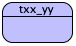
\includegraphics[height=20pt]{template/img/table} Es una tabla de color azul que representa una entidad fuerte o de negocio como en este caso puede ser \getElementById[Entidad]{local} o \getElementById[Entidad]{producto}. Si este tipo de tabla sólo tiene una llave(representada en el diagrama con negritas y un signo $+$) entonces se hará uso de una secuencia para mantener controlado el identificador que le puede ser asignado a los registros de este tipo de tablas.
		\item 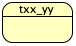
\includegraphics[height=20pt]{template/img/catalogo} Es una tabla de color amarillo que representa un catálogo en el sistema que se puede asociar a una entidad fuerta o de negocio como en este caso puede ser \getElementById[Entidad]{tipoOrden} o \getElementById[Entidad]{tipoProducto}. Este tipo de tablas no hacen uso de una secuencia dado que sus registros son insertados de forma controlada al crear la base de datos.
		\item 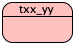
\includegraphics[height=20pt]{template/img/stateMachine} Es una tabla de color rosa en la que se almacenan los estados que intervienen o indican la condición de los registros de una entidad fuerte o de negocio. Este tipo de tablas no hacen uso de una secuencia dado que sus registros son insertados de forma controlada al crear la base de datos.
	\end{Citemize}


\section{Diagrama Relacional}
En esta sección se presenta el diagrama entidad relación de la base de datos\footnote{ver figura \ref{fig:bd}}.

\begin{figure}[hbtp!]
	\begin{center}
		\fbox{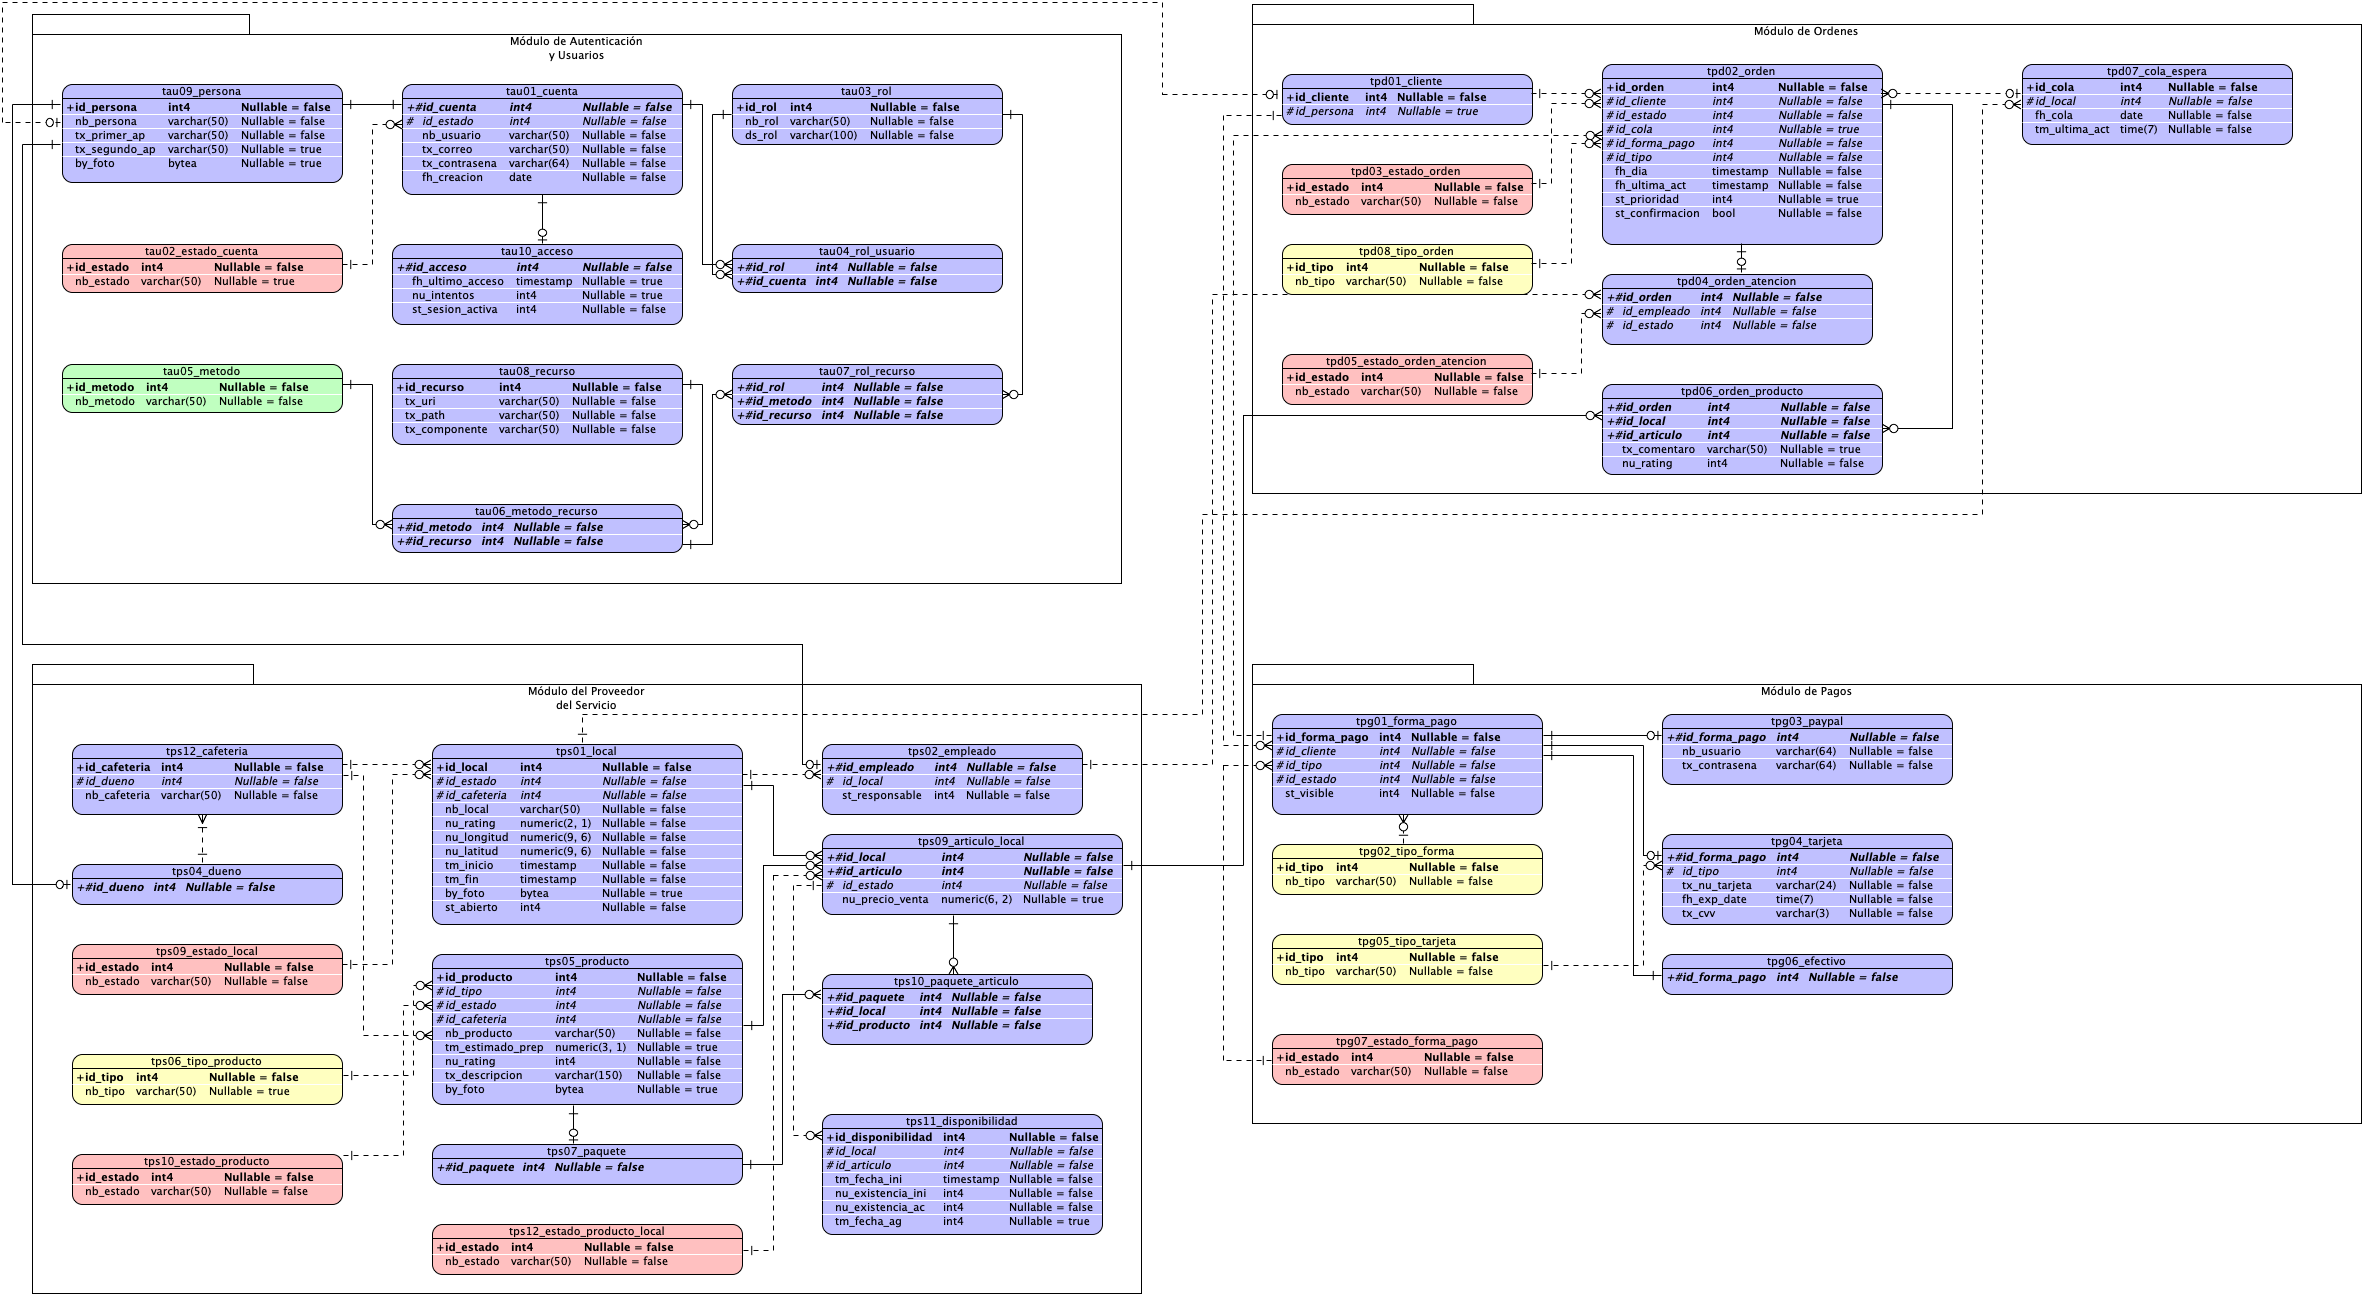
\includegraphics[angle=90,width=\textwidth,height=\textheight]{img/BD}}
		\caption{Diagrama ER de la Base de Datos}
		\label{fig:bd}
	\end{center}
\end{figure}

	
	\chapter{Arquitectura}
	\label{ch:arquitectura}
	%!TEX root = ../prueba.tex
En este capítulo se describe la arquitectura utilizada para la construcción y operación del sistema. Se hará uso de diagramas y algunas referencias bibliográficas para permitir el entendimiento adecuado de algunos conceptos formales.

\section{Arquitectura Física}

En esta sección se realizar la especificación técnica y física de la arquitectura sobre la cual la aplicación y el sistema funcionaran desde su puesta en producción. Dicha especificación se realiza utilizando como base la figura \ref{fig:arqFisica}.

\begin{figure}[hbtp!]
	\begin{center}
		\fbox{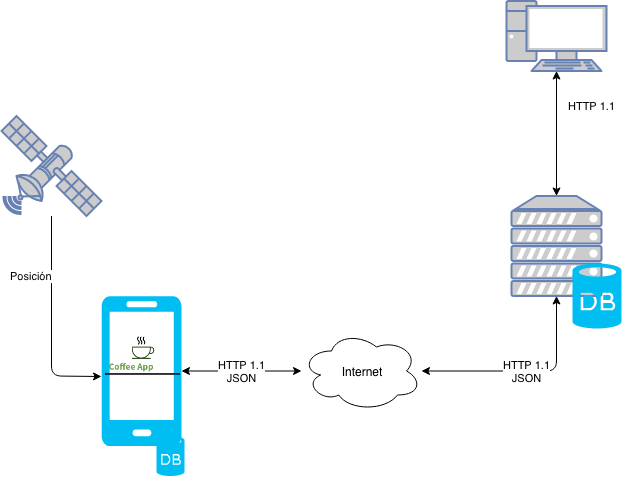
\includegraphics[width=.5\textwidth]{img/arqFisica}}
		\caption{Arquitectura Física del Sistema}
		\label{fig:arqFisica}
	\end{center}
\end{figure}

\subsection{Arquitectura Base}
El sistema está pensado para trabajar bajo un esquema centralizado tomando como base la arquitectura \textbf{Cliente-Servidor}. Esta arquitectura nos sirve como punto de partida debido a dos principales razones:
	\begin{itemize}
		\item Es requerido un punto centralizado(servidor) donde se almacene la mayor cantidad de información y que sea un punto de acceso para varios dispositivos.
		\item Es requerido hacer la implementación de dos diferentes clientes desde los cuales se tendrá acceso al servidor y por consiguiente a la información. El primer cliente consta de una aplicación móvil para dispositivos con sistema operativo Android, el segundo cliente consta de una aplicación web basada en \textit{Servlets} y \textit{JSP's}. 
	\end{itemize}

Se optó también por utilizar como base la arquitectura \textbf{Cliente - Servidor} ya que nos permite el uso del protocolo \textit{HTTP 1.1} para crear varios canales de comunicación entre los distintos clientes que accederán al sistema. El protocolo \textit{HTTP} nos define que para que exista comunicación entre el Cliente y el Servidor se debe hacer uso de dos mecanismos: una \textit{Petición} y una \textit{Respuesta}. A grandes rasgos, la petición está formada entre otras cosas por cabeceras, métodos y parámetros los cuales son enviados desde el cliente a través de la red hasta llegar al servidor el cual debe validar que la \textit{URL} desde la cual se hace la petición es válida. Posteriormente el servidor procesa la petición y en caso de existir el recurso y el método contenido en la petición le devolverá al cliente una respuesta con la información solicitada utilizando el formato indicado en el \textit{MIME/TYPE} de la respuesta.\\

Los actores que podrán acceder al sistema mediante la aplicación web son:
	\begin{itemize}
		\item El \getElementById[Stakeholder]{Jefe} dado que es el encargado de registrar, editar o eliminar la información de las cafeterías de las que es dueño así como sus respectivos locales y productos que se podrán encontrar en todos los locales de su franquicia.
		\item El \getElementById[Stakeholder]{Agente} dado que es el encargado de habilitar el acceso a las personas que tienen una cuenta bloqueada al sistema.
		\item El \getElementById[Stakeholder]{ResponsableDeLocal} dado que es el encargado de registrar la información de los productos que se ofertan en un local.
	\end{itemize}

Los actores que tendrán acceso a la aplicación móvil son:
	\begin{itemize}
		\item El \getElementById[Stakeholder]{Cliente} dado que desde su dispositivo únicamente podrá consultar información de las cafeterias, locales y productos publicados para realizar pedidos que serán atendidos por el personas de los locales, la aplicación móvil hará uso de dos mecanismos relevantes:
		\begin{itemize}
			\item El módulo GPS ya que cuando el cliente acceda a la aplicación se determinará su posición y con esto la ubicación de los locales más cercanos en un radio de 2 kilómetros.
			\item Una base de datos local que almacenará los pedidos que no han sido confirmados para que el cocinero de un local inicie su preparación.
		\end{itemize}
		\item El \getElementById[Stakeholder]{Cocinero} dado que a su tableta o a la tableta proporcionada por la cafetería, atenderá los pedidos e indicará la conclusión de su preparación para que se le entrege al cliente.
\end{itemize}

\subsection{Especificaciones Técnicas}
A continuación se especifican los detalles técnicos del sistema, es decir, el Hardware y Software requerido para que el sistema opere de forma estable.

\subsubsection{Servidor}
El servidor tiene las siguientes especificaciones:
	\begin{description}
		\item[Marca:]Servidor Dell PowerEdge T30.
		\item[Procesador:]Intel Xeon E3-1225V5 3.30GHz.
		\item[Memoria RAM:]8GB DDR4.
		\item[Disco Duro:]1TB.
		\item[Sistema Operativo:] CentOS 7.4-1708.
	\end{description}

\subsection{Base de Datos}
	\begin{description}
		\item[SGBD:] Postgresql 9.4
	\end{description}

\subsubsection{Cliente Web}
La aplicación web puede ser utilizada bajo las siguientes especificaciones:
	\begin{description}
		\item[Navegadores Compatibles:]\hspace{0.5pt}
			\begin{itemize}
				\item Google Chrome Versión $\geq$ 70.0.3538.
				\item Mozilla Firefox $\geq$ 63.0.
				\item Safari $\geq$ 12.0.
			\end{itemize}
		\item[Resolución:]\hspace{0.5pt}
			\begin{itemize}
				\item Mínima:1027x768
				\item Máxima:1920x1080
			\end{itemize}
	\end{description}

\subsubsection{Cliente Móvil}
La aplicación móvil puede ser utilizada bajo las siguientes especificaciones:
	\begin{description}
		\item[Sistema Operativo:] Android >= 5.0 Lollipop.
		\item[Memoria RAM:] 2GB.
		\item[Almacenamiento:] 16 GB.
	\end{description}


\subsection{Arquitectura Lógica}
Una vez descrita la arquitectura física del sistema, es requerido indicar y especificar cómo será construido. En general las aplicaciones que se van a desarrollar utilizarán una arquitectura a capas. En la figura \ref{fig:arqLogica} se pueden observar las capas del sistema en los diferentes clientes(o aplicaciones) y posteriormente se hará una descripción de la función de cada capa.\\

\begin{figure}[hbtp!]
	\begin{center}
		\fbox{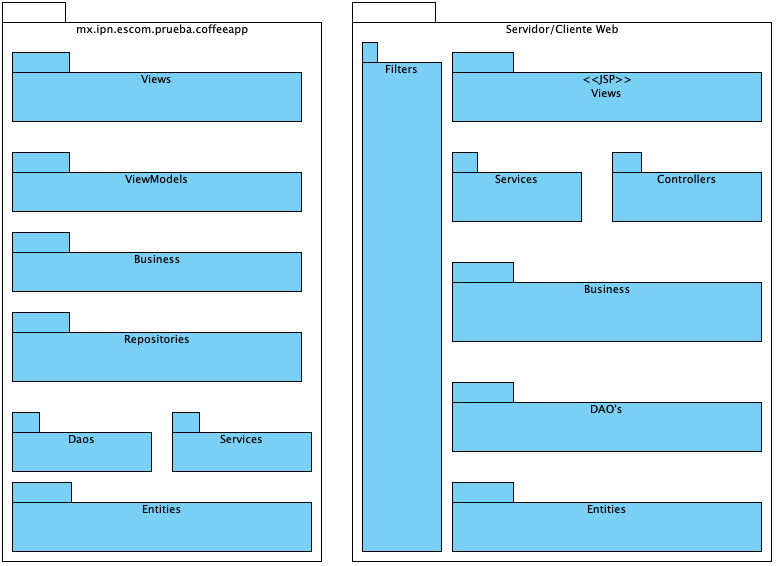
\includegraphics[width=0.8\textwidth]{img/arqLogicaP}}
		\caption{Arquitectura Lógica del Sistema}
		\label{fig:arqLogica}
	\end{center}
\end{figure}

\subsubsection{Arquitectura Lógica del Servidor/Aplicación Web}
Como se mencionó al iniciar esta sección, las aplicaciones están construidas a partir de una arquitectura multi capa.El servidor(paquete del lado derecho en la figura \ref{fig:arqLogica}) está dividido en las siguientes capas:
	\begin{description}
		\item[Entities:] En esta capa se definen las clases que se utilizarán para la manipulación de las estructuras de datos de la base de datos.
		\item[DAO's:] En esta capa se definen las clases que sirven de interacción entre la capa de \textit{business} y la capa de \textit{entities} para la recolección de datos utilizando el patrón de diseño DAO.
		\item[Business:] En esta capa se definen las clases que sirven para la abstracción de las reglas de negocio así como de las operaciones y funciones disponibles en el sistema.
		\item[Services:] En esta capa se definen las clases que corresponden al servicio RESTful que será consumido por la aplicación móvil.
		\item[Controllers:] Está capa tiene el propósito establecido para la capa de \textit{Controlador} en el patrón de diseño \textit{MVC} en donde se va a administrar el flujo de datos que hay entre la capa \textit{views} y la capa \textit{business}.
		\item[Views:] Está capa contiene los archivos JPA's que presentan las interfaces de usuario para la aplicación web.
	\end{description}
	
Como observación general, en el paquete de \textit{Business} se creará una clase que lleva por nombre \textit{GenericBs} el cual se compone de otra clase en el paquete \textit{DAO's} que lleva por nombre \textit{GenericDao}, esta última clase implementa los métodos genéricos para actualizar, guardar o encontrar una entidad en la base de datos, por esta razón todas las clases que se encuentren en un paquete con terminación \textit{bs} heredan de la clase \textit{GenericBs}.\\
	
En la figura \ref{fig:maqservarq} se presenta un diagrama de clases que tiene como principal propósito mostrar las clases y paquetes que se implementarán para el módulo de autenticación y usuarios.

\begin{figure}[hbtp!]
	\begin{center}
		\fbox{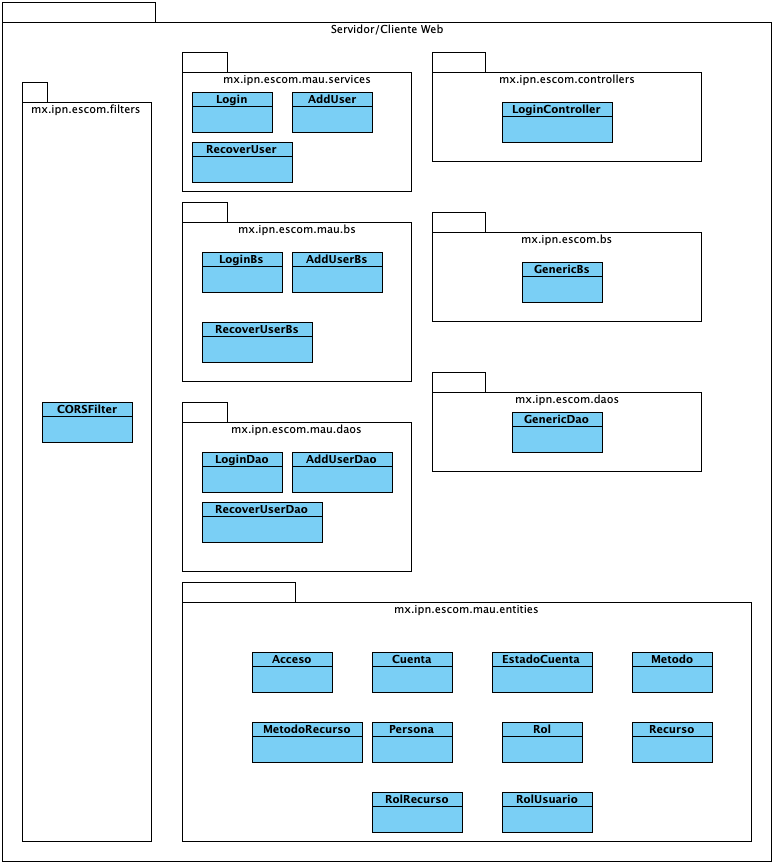
\includegraphics[width=0.8\textwidth]{img/MAU_SERV_ARQ}}
		\caption{Arquitectura Lógica en el Servidor del Módulo de Autenticación y Usuarios.}
		\label{fig:maqservarq}
	\end{center}
\end{figure}

	
\subsubsection{Arquitectura Lógica de la Aplicación Móvil}
La aplicación móvil se va a construir con base en el patrón arquitectónico \textit{MVC}, agregando una capa la cual tiene como principal propósito administrar las peticiones que se van a mandar al servidor y proveer de datos a la capa de \textit{Models}. Estas capas se pueden observar en la figura \ref{fig:arqLogica} del lado izquierdo en el paquete de Cliente Móvil. Así mismo dado que la aplicación móvil es nativa del sistema operativo Android, se hará uso de algunos patrones de diseño establecidos por \textit{Google} para el comportamiento de algunos componentes como lo es el patrón \textit{Adapter} para el componente \textit{Recycler View}. A continuación se hace la descripción de las capas del patrón MVVM:
	\begin{description}
		\item[Views:] En este paquete se encuentran aquellas clases que construyen las interfaces de usuario y se actualizan con respecto a los eventos o cambios de datos de la capa \textit{ViewModel}.
		\item[ViewModels:] En este paquete se encuentran las clases que identifican un cambio en el modelo y actualizan la interfaz.
		\item[Business:] En este paquete se encuentran las clases que abstraen e implementan algunas de las reglas de negocio que intervienen directamente con el éxito o fracaso de una operación en el sistema.
		\item[Repositories:] En este paquete se encuentran las clases que permiten la conexión a la base de datos local o realizar la conexión con el servicio web para la búsqueda e inserción de datos.
		\item[Daos:] En este paquete se encuentran las clases que, de acuerdo con el patrón de diseño \textit{DAO}, permite el acceso a los datos almacenados en el dispositivo de forma local.
		\item[Services:] En este paquete se encuentran las clases que permiten la conexión al servidor para la recolección e inserción de datos en el sistema.
		\item[Entities:] En este paquete se encuentran las clases que abstraen las entidades de negocio que se muestran al cliente o se insertan en el sistema.
	\end{description}


\begin{figure}[hbtp!]
	\begin{center}
		\fbox{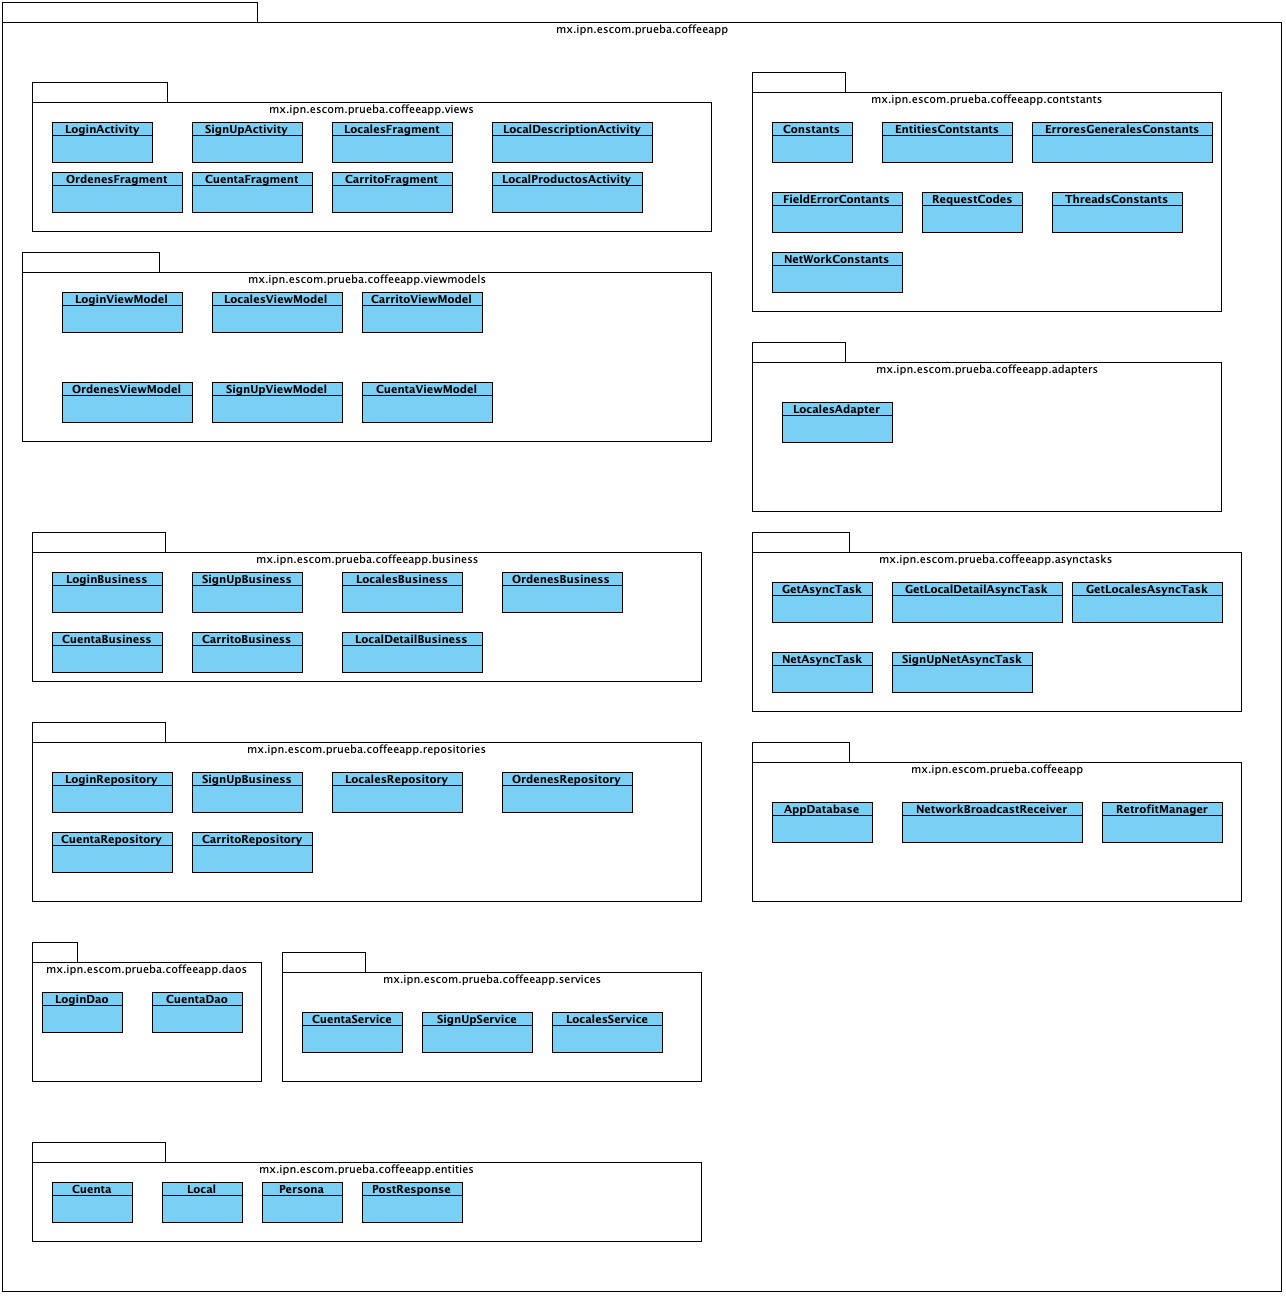
\includegraphics[width=\textwidth]{img/APP_ARQ}}
		\caption{Arquitectura Lógica de la Aplicación Móvil}
		\label{fig:arqLogApp}
	\end{center}
\end{figure}



	
	\chapter{Diagramas de Secuencia}
	\label{ch:diagramasDeSecuencia}
	%!TEX root = ../prueba.tex
En este capítulo se describen los diagramas de secuencia que indican la forma en que los diferentes objetos se comunican entre si para presentar información en la pantalla correspondiente.

\section{SEQ01-Diagrama de Secuencia de Login}
\begin{description}
	\item[Diagrama:]\hspace{1pt}
	\begin{figure}[hbtp!]
		\begin{center}
			\fbox{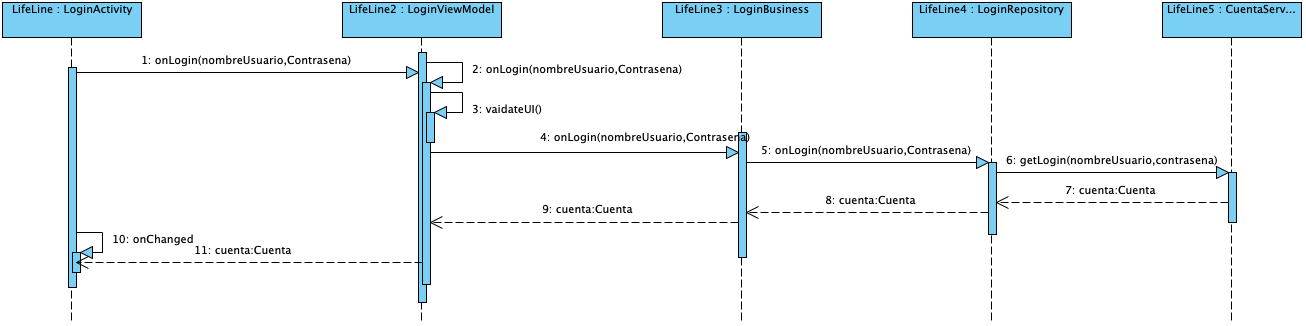
\includegraphics[width=\textwidth]{seq/loginSeq}}
			\caption{Diagrama de Secuencia de Login}
			\label{fig:SEQ01}
		\end{center}
	\end{figure}
	
	\item[Caso de Uso:]\getElementById[CU]{CUMAU1}

\end{description}



\section{SEQ02-Diagrama de Secuencia de Consulta de Locales}

\begin{description} 
	\item[Diagrama:]\hspace{1pt}
	\begin{figure}[hbtp!]
		\begin{center}
			\fbox{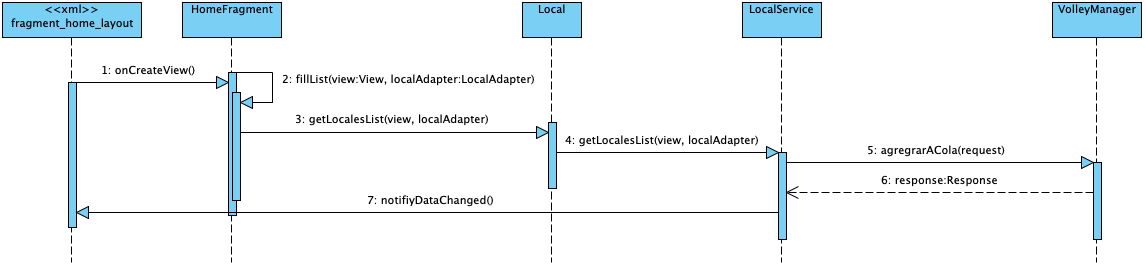
\includegraphics[width=\textwidth]{seq/localesSeq}}
			\caption{Diagrama de Secuencia de Consulta de Locales}
			\label{fig:SEQ02}
		\end{center}
	\end{figure}
	
	\item[Caso de Uso:]\getElementById[CU]{CUMC3}
\end{description}
	
	\appendix
	
	\chapter{Mensajes}
	\label{ch:mensajes}
	%!TEX root = ../prueba.tex
En este capítulo se especifican los mensajes que el sistema utiliza para notificar a los actores sobre el estado sobre las operaciones que están realizando.

%%%%%%%%%%%%%%%%%%
%%%%%% Mensajes Generales
%%%%%%%%%%%%%%%%%%

%Tipos de Mensajes
%Operación/Notificación/Alerta/Error
\begin{mensaje}{MSG1}{Operación Exitosa}{Operación}
	\item[Descripción:]Este mensaje tiene la finalidad de comunicar que la acción se ha concretado de forma exitosa.
	\item[Redacción:]La operación se realizó de forma exitosa.
	\item[Parámetros:] 
	\begin{Citemize}
 			\item 
		\end{Citemize}
	\item[Ejemplo:] 
\end{mensaje}s

\begin{mensaje}{MSG2}{Operación Fallida}{Error}
	\item[Descripción:]Este mensaje tiene la finalidad de comunicar que hubo un error y por lo tano la acción no se pudo concretar de forma exitosa.
	\item[Redacción:]Error, la operación no se pudo llevar a cabo.
	\item[Parámetros:] 
	\begin{Citemize}
 			\item 
		\end{Citemize}
	\item[Ejemplo:] 
\end{mensaje}

\begin{mensaje}{MSG3}{Elementos No Disponibles}{Error}
	\item[Descripción:]Este mensaje tiene la finalidad de comunicar que los elementos solicitados no están disponibles.
	\item[Redacción:]¡No hay elementos para mostrarte!
	\item[Parámetros:] 
	\begin{Citemize}
 			\item 
		\end{Citemize}
	\item[Ejemplo:] 
\end{mensaje}

\begin{mensaje}{MSG4}{Duplicado de Información}{Error}
	\item[Descripción:]Este mensaje tiene la finalidad de comunicar que hubo un error debido a un elemento duplicado, por lo que la acción no se puede llevar acabo.
	\item[Redacción:]¡Ya existe un elemento con la misma información!
	\item[Parámetros:] 
	\begin{Citemize}
 			\item 
		\end{Citemize}
	\item[Ejemplo:] 
\end{mensaje}

\begin{mensaje}{MSG5}{Falta dato obligatorio}{Error}
	\item[Descripción:]Este mensaje tiene la finalidad de comunicar que hubo un error debido a que hace falta un dato considerado como obligatorio, por lo que la acción no se puede llevar acabo.
	\item[Redacción:]"!Error¡ Los campos marcados con * son obligatorios, 
favor de ingresar el campo faltante."
	\item[Parámetros:] 
	\begin{Citemize}
 			\item 
		\end{Citemize}
	\item[Ejemplo:] 
\end{mensaje}

\begin{mensaje}{MSG6}{Formato de campo incorrecto}{Error}
	\item[Descripción:]Este mensaje tiene la finalidad de comunicar que hubo un error debido a que el dato ingresado posee un formato incorrecto acorde a la regla(s) de negocio establecidas, por lo que la acción no se puede llevar acabo.
	\item[Redacción:]El dato ingresado es incorrecto, favor de ingresar un dato válido.
	\item[Parámetros:] 
	\begin{Citemize}
 			\item 
		\end{Citemize}
	\item[Ejemplo:] 
\end{mensaje}

\begin{mensaje}{MSG7}{Eliminar elemento}{Alerta}
	\item[Descripción:]Este mensaje tiene la finalidad de comunicar que se pretende eliminar un elemento, por lo que pregunta por la confirmación de esta operación.
	\item[Redacción:]¿Desea eliminar el ELEMENTO?
	\item[Parámetros:] \hspace{0.1pt}
	\begin{Citemize}
 			\item ELEMENTO
		\end{Citemize}
	\item[Ejemplo:] 
\end{mensaje}

\begin{mensaje}{MSG8}{Longitud de campo incorrecta}{Error}
	\item[Descripción:]Este mensaje tiene la finalidad de comunicar que hubo un error debido a que la longitud del dato ingresado no concuerda con lo establecido en la regla(s) de negocio establecidas, por lo que la acción no se puede llevar acabo.
	\item[Redacción:]La longitud de campo es incorrecta.
	\item[Parámetros:] 
	\begin{Citemize}
 			\item 
		\end{Citemize}
	\item[Ejemplo:] 
\end{mensaje}

\begin{mensaje}{MSG9}{No existe información necesaria en el sistema}{Alerta}
	\item[Descripción:]Este mensaje tiene la finalidad de comunicar que no existe la información necesaria en el sistema para poder llevar acabo la operación.
	\item[Redacción:]Falta información necesaria en el sistema para poder realizar está operación.
	\item[Parámetros:] 
	\begin{Citemize}
 			\item 
		\end{Citemize}
	\item[Ejemplo:] 
\end{mensaje}

\begin{mensaje}{MSG10}{Confirmación de operación}{Alerta}
	\item[Descripción:]Este mensaje tiene la finalidad de comunicar que se pretende realizar una operación, por lo que se solicita la confirmación de la operación para poder llevarla acabo.
	\item[Redacción:]¿Está seguro que requiere ACCION ELEMENTO ?
	\item[Parámetros:] \hspace{0.1pt}
	\begin{Citemize}
 			\item ACCION
			\item ELEMENTO
		\end{Citemize}
	\item[Ejemplo:] 
\end{mensaje}

\begin{mensaje}{MSG11}{Campo vacio}{Error}
	\item[Descripción:]Este mensaje tiene la finalidad de comunicar que hubo un error debido a que un campo en particular no contiene datos, por lo que la operación no se puede llevar acabo.
	\item[Redacción] Error, Este campo está vacío.
	\item[Parámetros] No aplica
\end{mensaje}


%%%%%%%%%%%%%%%%%%
%%%%%% Mensajes del modulo
%%%%%%%%%%%%%%%%%%
\begin{mensaje}{MSGMAU1}{El nombre de usuario no posee cuenta una cuenta asociada}{Error}
	\item[Descripción:] Este mensaje tiene la finalidad de comunicar que el nombre de usuario insertado para iniciar sesión no posee una cuenta asociada.
	\item[Redacción] Error: Cuenta no encontrada.
	\item[Parámetros] No aplica.
\end{mensaje}

\begin{mensaje}{MSGMAU2}{La contraseña insertada no coincide con la cuenta asociada}{Error}
	\item[Descripción:] Este mensaje tiene la finalidad de comunicar que la contraseña insertada para iniciar sesión no coincide con la contraseña de la cuenta asociada.
	\item[Redacción] Error: Contraseña no coincide.
	\item[Parámetros] No aplica.
\end{mensaje}

\begin{mensaje}{MSGMAU3}{La cuenta posee el estado bloqueado}{Error}
	\item[Descripción:] Este mensaje tiene la finalidad de comunicar que no se puede iniciar sesión con la cuenta asociada, ya que posee el estado Bloqueado.
	\item[Redacción] Error: Cuenta bloqueada.
	\item[Parámetros] No aplica.
\end{mensaje}

\begin{mensaje}{MSGMAU4}{El nombre de usuario ya posee una cuenta asociada}{Error}
	\item[Descripción:] Este mensaje tiene la finalidad de comunicar que no se puede regsitrar una cuenta haciendo uso de este nombre de usuario, debido a que ya existe una cuenta asociada a este nombre. 
	\item[Redacción] Error: Nombre de usuario no disponible.
	\item[Parámetros] No aplica.
\end{mensaje}

%%%%%%%%%%%%%%%%%%
%%%%%% Mensajes del modulo
%%%%%%%%%%%%%%%%%%
\begin{mensaje}{MSGMOR1}{Geolocalización Inhabilitada}{Alerta}
	\item[Descripción:]Este mensaje tiene la finalidad de indicarle al Cliente que al no tener habilitada la geolocalización en su dispositivo móvil no es posible realizar la búsqueda de locales cerca de su posición.
	\item[Redacción]No es posible determinar tu ubicación porque el servicio está inhabilitado
	\item[Parámetros] No aplica.
\end{mensaje}

\begin{mensaje}{MSGMOR2}{No hay locales cerca}{Alerta}
	\item[Descripción:]Este mensaje tiene la finalidad de indicarle al Cliente que no fue posible encontrar al menos un local cerca de su ubicación.
	\item[Redacción]No hay locales cerca de tu ubicación.
	\item[Parámetros] No aplica.
\end{mensaje}

\begin{mensaje}{MSGMOR3}{Ubicación No Exacta}{Alerta}
	\item[Descripción:]Este mensaje tiene la finalidad de indicarle al Cliente que la dirección de un local no es completamente exacta.
	\item[Redacción]Advertencia, la dirección desplegada no es exacta.
	\item[Parámetros] No aplica.
\end{mensaje}

\begin{mensaje}{MSGMOR4}{Cuenta No Encontrada}{Error}
	\item[Descripción:]Este mensaje tiene la finalidad de comunicar que hubo un error al tratar de encontrar una cuenta asociada al nombre de usuario proporcionado.
	\item[Redacción]Error, no existe cuenta asociada al nombre de usuario ingresado.
	\item[Parametros] No aplica.
\end{mensaje}




	
	\newpage
	\clossing
	
	%\saveData

\end{document}
